%% ----------------------------------------------------------------
%% Report.tex
%% ---------------------------------------------------------------- 
\documentclass{ecsreport}      % Use the Report Style
%\documentclass{report}
\graphicspath{{../Figures/}}   % Location of your graphics files
\usepackage{pgfplots}
\usepackage{natbib}  % Use Natbib style for the refs.
\usepackage{import}
%\usepackage{subfig}
\usepackage{subcaption}				
\hypersetup{colorlinks=true}   % Set to false for black/white printing
%% ----------------------------------------------------------------
%% Definitions.tex
%% ---------------------------------------------------------------- 
\newcommand{\BibTeX}{{\rm B\kern-.05em{\sc i\kern-.025em b}\kern-.08em T\kern-.1667em\lower.7ex\hbox{E}\kern-.125emX}}






%% People
\newcounter{address}
\setcounter{address}{1}
\renewcommand{\theaddress}{\textsuperscript{\fnsymbol{address}}}
\newcommand{\address}[1]{\refstepcounter{address}\theaddress#1\\}
\newcommand{\Name}[3]{\texorpdfstring{\href{mailto:#3}{#2}#1}{#2}\xspace}
\newcommand{\SteveRGunn}[1]{\Name{#1}{Steve R. Gunn}{S.R.Gunn@ecs.soton.ac.uk}}

%% Dingbats
\newcommand{\tick}{\ding{51}}
\newcommand{\cross}{\ding{55}}


%% My definitions
\newcommand{\nPossRes}{\ensuremath{m}\xspace}
\newcommand{\possResVec}{\ensuremath{D}\xspace}
\newcommand{\realPossResVec}{\ensuremath{R}\xspace}
\newcommand{\possCirclePos}{\ensuremath{X}\xspace}
\newcommand{\nPossCirclePos}{\ensuremath{n}\xspace}
\newcommand{\workResVec}{\ensuremath{Z}\xspace}
\newcommand{\workIndex}{\ensuremath{i}\xspace}
\newcommand{\gtIndex}{\ensuremath{j}\xspace}
\newcommand{\gtIndexCons}{\ensuremath{k}\xspace}
\newcommand{\resChange}{\ensuremath{RC(\workResVec_{\workIndex,\gtIndex})}\xspace}
\newcommand{\workModType}[1]{\ensuremath{M_#1}\xspace}
\newcommand{\modType}{\workModType {\text{type}}}
\newcommand{\consInc}{\workModType{I}}
\newcommand{\consDec}{\workModType{D}}
\newcommand{\consCon}{\workModType{C}}
\newcommand{\resSym}{\workModType{{RS}}}
\newcommand{\trueSym}{\workModType{{TS}}}



\newcommand{\inputTikZ}[2]{%  
     \scalebox{#1}{\input{#2}}  
}




%% Calculus
\newcommand{\pd}[2]{\ensuremath{\frac{\partial #1}{\partial #2}}\xspace}
\newcommand{\fd}[2]{\ensuremath{\frac{d #1}{d #2}}\xspace}
\newcommand{\dint}{\ensuremath{\int\!\!\!\int}\xspace}
\newcommand{\tint}{\ensuremath{\int\!\!\!\int\!\!\!\int}\xspace}

%% Math Sets
\newcommand{\Q}[1]{\ensuremath{\mathbb{#1}}\xspace}
\newcommand{\R}{\Q{R}}

%% Matrix, Vector
\newcommand{\V}[1]{\ensuremath{\boldsymbol{#1}}\xspace}
\newcommand{\M}[1]{\ensuremath{\boldsymbol{#1}}\xspace}
\newcommand{\0}{\V{0}}
\newcommand{\1}{\V{1}}
\newcommand{\I}{\M{I}}

%% Math Functions
\newcommand{\F}[1]{\ensuremath{\mathrm{#1}}\xspace}
\newcommand{\sgn}{\F{sgn}}
\newcommand{\tr}{\F{trace}}
\newcommand{\diag}{\F{diag}}

%% Math Names
\newcommand{\N}[1]{\ensuremath{\mathit{#1}}\xspace}

%% Data
\newcommand{\mc}[1]{\ensuremath{\mathcal{#1}}\xspace}
\newcommand{\Hyp}{\mc{H}}
\newcommand{\D}{\mc{D}}

%% Kernel
\newcommand{\K}{\M{K}}
\newcommand{\eins}{\texorpdfstring{\ensuremath{\epsilon}}{\textepsilon}-insensitive\xspace}
\newcommand{\e}{\ensuremath{\epsilon}\xspace}
\newcommand{\Bxi}{\ensuremath{\boldsymbol{\xi}}\xspace}
\newcommand{\Kanova}{\ensuremath{\mathit{K_{ANOVA}}}\xspace}
\newcommand{\Kspline}{\ensuremath{\mathit{K_{spline}}}\xspace}

%% Bayesian
\newcommand{\MP}{\ensuremath{\mathit{{\scriptscriptstyle \hspace{-1.5pt}M\hspace{-1.5pt}P}}}\xspace}
\newcommand{\ML}{\ensuremath{\mathit{{\scriptscriptstyle \hspace{-1.5pt}M\hspace{-1.5pt}L}}}\xspace}
\newcommand{\Qw}{\ensuremath{Q_{\w}(\w)}\xspace}
\newcommand{\Qa}{\ensuremath{Q_{\Ba}(\Ba)}\xspace}
\newcommand{\Qb}{\ensuremath{Q_{\beta}(\beta)}\xspace}
\newcommand{\wMPab}{\ensuremath{\w_{\MP|\bar {\Ba},\bar \beta}}\xspace}
\newcommand{\wMP}{\ensuremath{\w_{\MP}}\xspace}
\newcommand{\yMP}{\ensuremath{y_{\MP}}\xspace}
\newcommand{\BaMP}{\ensuremath{\Ba_{\hspace{1pt}\MP}}\xspace}
\newcommand{\aMP}{\ensuremath{\alpha_{\hspace{1pt}\MP}}\xspace}
\newcommand{\bMP}{\ensuremath{\beta_{\hspace{1pt}\MP}}\xspace}
\newcommand{\Sab}{\ensuremath{\M{\Sigma}_{\bar \Ba,\bar \beta}}\xspace}
\newcommand{\Ba}{\ensuremath{\boldsymbol{\alpha}}\xspace}
\newcommand{\Bb}{\ensuremath{\boldsymbol{\beta}}\xspace}
\newcommand{\Bm}{\ensuremath{\boldsymbol{\mu}}\xspace}
\newcommand{\BL}{\ensuremath{\boldsymbol{\Lambda}}\xspace}
\newcommand{\BPhi}{\ensuremath{\boldsymbol{\Phi}}\xspace}
\newcommand{\SMP}{\ensuremath{\M{\Sigma}_{\MP}}\xspace}

\newcommand{\Pa}{\ensuremath{P(\alpha|\mathcal{H})}\xspace}
\newcommand{\Pb}{\ensuremath{P(\beta|\mathcal{H})}\xspace}
\newcommand{\Pab}{\ensuremath{P(\alpha,\beta|\mathcal{H})}\xspace}
\newcommand{\Pw}{\ensuremath{P(\w|\mathcal{H})}\xspace}
\newcommand{\PD}{\ensuremath{P(\D|\mathcal{H})}\xspace}
\newcommand{\PwIa}{\ensuremath{P(\w|\alpha,\mathcal{H})}\xspace}
\newcommand{\PDIwb}{\ensuremath{P(\D|\w,\beta,\mathcal{H})}\xspace}
\newcommand{\PDwab}{\ensuremath{P(\D,\w,\alpha,\beta|\mathcal{H})}\xspace}
\newcommand{\PDIw}{\ensuremath{P(\D|\w,\mathcal{H})}\xspace}
\newcommand{\PwID}{\ensuremath{P(\w|\D,\mathcal{H})}\xspace}
\newcommand{\PwabID}{\ensuremath{P(\w,\alpha,\beta|\D,\mathcal{H})}\xspace}

\newcommand{\PanH}{\ensuremath{P(\alpha)}\xspace}
\newcommand{\PbnH}{\ensuremath{P(\beta)}\xspace}
\newcommand{\PabnH}{\ensuremath{P(\alpha,\beta)}\xspace}
\newcommand{\PwnH}{\ensuremath{P(\w)}\xspace}
\newcommand{\PDnH}{\ensuremath{P(\D)}\xspace}
\newcommand{\PwIanH}{\ensuremath{P(\w|\alpha)}\xspace}
\newcommand{\PDIwbnH}{\ensuremath{P(\D|\w,\beta)}\xspace}
\newcommand{\PDwabnH}{\ensuremath{P(\D,\w,\Ba,\beta)}\xspace}
\newcommand{\PDIwnH}{\ensuremath{P(\D|\w)}\xspace}
\newcommand{\PwIDnH}{\ensuremath{P(\w|\D)}\xspace}
\newcommand{\PwabIDnH}{\ensuremath{P(\w,\alpha,\beta|\D)}\xspace}

\newcommand{\PDwBab}{\ensuremath{P(\D,\w,\Ba,\beta|\mathcal{H})}\xspace}
\newcommand{\PwIBa}{\ensuremath{P(\w|\Ba,\mathcal{H})}\xspace}
\newcommand{\PBab}{\ensuremath{P(\Ba,\beta|\mathcal{H})}\xspace}
\newcommand{\PwBabID}{\ensuremath{P(\w,\Ba,\beta|\D,\mathcal{H})}\xspace}

\newcommand{\PBanH}{\ensuremath{P(\Ba)}\xspace}
\newcommand{\PwIBanH}{\ensuremath{P(\w|\Ba)}\xspace}

%% Snakes
\newcommand{\Esnake}{\ensuremath{\mathit{E_{snake}}}\xspace}
\newcommand{\Eimage}{\ensuremath{\mathit{E_{image}}}\xspace}
\newcommand{\Econt}{\ensuremath{\mathit{E_{cont}}}\xspace}
\newcommand{\Ecurv}{\ensuremath{\mathit{E_{curv}}}\xspace}
\newcommand{\Eint}{\ensuremath{\mathit{E_{int}}}\xspace}
\newcommand{\Eext}{\ensuremath{\mathit{E_{ext}}}\xspace}
\newcommand{\Eterm}{\ensuremath{\mathit{E_{term}}}\xspace}
\newcommand{\Eline}{\ensuremath{\mathit{E_{line}}}\xspace}
\newcommand{\Eedge}{\ensuremath{\mathit{E_{edge}}}\xspace}
\newcommand{\Econ}{\ensuremath{\mathit{E_{con}}}\xspace}
\newcommand{\Eangle}{\ensuremath{\mathit{E_{angle}}}\xspace}
\newcommand{\Elshape}{\ensuremath{\mathit{E_{lshape}}}\xspace}
\newcommand{\Eedgedir}{\ensuremath{\mathit{E_{edgedir}}}\xspace}
\newcommand{\Emodel}{\ensuremath{\mathit{E_{model}}}\xspace}
\newcommand{\wte}{\ensuremath{\mathit{w_{term}}}\xspace}
\newcommand{\wli}{\ensuremath{\mathit{w_{line}}}\xspace}
\newcommand{\wed}{\ensuremath{\mathit{w_{edge}}}\xspace}
\newcommand{\wco}{\ensuremath{\mathit{w_{con}}}\xspace}

%% Environments
\newcounter{alg}
\newenvironment{algorithm}[1]
{
    \stepcounter{alg}
    \begin{table}[htb]
    \centering
    \begin{tabular}[t]{ll}
    \hline&\\
    \multicolumn{2}{l}{\bf Algorithm \arabic{alg}: #1}\\&\\
} {
    &\\
    \hline
    \end{tabular}
    \end{table}
}            % Include your abbreviations
%% ----------------------------------------------------------------
\begin{document}
\frontmatter
\title      {Crowdsourcing Experiments}
\authors    {\texorpdfstring
             {\href{mailto:cebsp@bristol.ac.uk}{Barry Park}}
             {Barry Park}
            }
\addresses  {\groupname\\\deptname\\\univname}
\date       {\today}
\subject    {}
\keywords   {}
\maketitle
\begin{abstract}
This work is all about \dots
\end{abstract}
\tableofcontents
\listoffigures
\listoftables
%\lstlistoflistings
%\listofsymbols{ll}{$w$ & The weight vector}
%\acknowledgements{Thanks to no one.}
%\dedicatory{To \dots}

%%-----------------------------------------------------------------
%%COMMANDS
%functions
\newcommand{\funcx}{\ensuremath{f(x)}}
\newcommand{\probx}{\ensuremath{p(x)}}
\newcommand{\propx}{\ensuremath{q(x)}}
\newcommand{\expectation}[1]{\ensuremath{\mathbb{E}[#1]}}
\newcommand{\sample}[2][x]{\ensuremath{#1^{(#2)}}}
\newcommand{\approxiw}[2][x]{\ensuremath{\tilde{w}(\sample[#1]{#2})}}
\newcommand{\normiw}[2][x]{\ensuremath{\ensuremath{w(\sample[#1]{#2})}}}
%%-----------------------------------------------------------------





\mainmatter
%% ----------------------------------------------------------------
%\include{introduction}
%\chapter{Data Fusion} \label{Chapter: DataFusion}

\section{Summaries}

One difficulty I have found with analysing the results, is how to summarise the results of data fusion. 
Upon completion of the data fusion using a certain number of crowdsourced reports, we arrive at a posterior distribution. 
This distribution tells us the probability of the circle being found within a certain region. 

There are two difficulties. 
The first is how to summarise a single posterior distribution, as often the distribution is non-symmetric. 

\subsection{Expectation Values}

For some function \funcx, under a probability distribution \probx, then the average value of \funcx is called the Expectation Value, written as \expectation{\funcx}. 
For a discrete distribution, the expectation is given by

\begin{equation}\label{Equation: discrete_expectation}
\expectation{\funcx}=\sum\limits_x p(x)f(x)
\end{equation}

and for a continuous distribution we take the integral

\begin{equation}\label{•}
\expectation{\funcx}=\int \probx\funcx dx
\end{equation}

When a finite number of samples $N$ are drawn from the probability distribution $p(x)$, then the expectation can be approximated by 

\begin{equation}\label{Equation: discrete_sample_expectation}
\expectation{\funcx}\simeq\frac{1}{N}\sum\limits_{n=1}^N f(x_n)
\end{equation}

The expectation value of a function can be viewed as a weighted average.

\fref{Figure: Means} shows a Gaussian and Gamma probability functions, and the corresponding expectation value $\mathbb{E}[f]$ where $x=\lbrace0,1,...,N\rbrace$ with $f(x)=x/N$ and $N=1000$. 

%\begin{figure}
%	\centering
%	\setlength\figureheight{6cm} 
%	\setlength\figurewidth{10cm}
%	\input{gaussian_and_gamma_means.tikz}
%	\caption{The expected values, or means, of two probability distributions}
%	\label{Figure: Means}
%\end{figure}

\subsection{Point Estimates from Posterior Distributions}

Point estiamtes are useful for reporting a single summary value of the distribution. 
Probably the most common is to take the expected value of the distribution, as shown in \fref{Figure: Means} which gives us the mean value of the parameter that distribution describes. 

Another common point estimate is the Maximum A-Posteriori of the distribution, which corresponds to a mode of the distribution.

For data fusion, the expected value is commonly reported as it is the mean estiamtion we are interested in 


\subsection{Spread of values}
One standard measure for how much a distribution varies from its mean is variance. The varaince of a function $f(x)$ can be defined in terms of expectations as 
\[ 
var[f]=\mathbb{E}[(f(x)-\mathbb{E}[f(x)])^2]
\]

which can be rewritten as

\[ 
var[f]=\mathbb{E}[f(x)^2]-\mathbb{E}[f(x)]^2
\]


For a posterior distribution, another standard measure of the spread around the mean of the distribution is the use of Bayesian confidence intervals, also known as credible intervals. 
A credible interval defines a region of a distribution where there is a defined probability that the true parameter being estimated lies within. 
For example, if the probability that a variable $x$ lies between $0.1$ and $0.9$ is $0.95$, then $0.1 \leq  x \leq 0.9$ is a $95\% $ confidence interval

More formally, we can define a credible interval of a probability distribution $p(x)$ as

\[ 
\int\limits_L^U p(x)=1-\alpha
\]

where $U$ is the upper credible bound, $L$ is the lower credible bound, and $\alpha$ sets the value of the credible interval. 
Credible intervals in more than 1 dimension are called credible regions. 
Credible regions are invariant under reparametrization A common credible interval is to centre the interval on the posterior mean. 
If we select the credible interval with minimum size, this region is called the highest probability density (HPD) region. 
HPDs are not invariant under reparametrization, but an HPD will always be a credible interval afterwards. 

Calculating the HPD of ran arbitrary distribution can be computationally challenging, and is often achieved through sampling the distribution



\section{Sampling Distributions}

In most real applications, it is difficult to analytically integrate a distribution, as a closed form solution may not exist. 
We therefore have to resort to numerical integration. 

A relatively simple brute force approach is to evaluate the distribution at a series of evenly spaced points, and then interpolate between these using easy to integrate polynomials. 

These methods can give accurate approximations of the integral when the spacing between points is small, but as the state space increases, the function evaluations grow exponentially.

A second approach to approximating an integral is the use of Monte Carlo (MC) sampling,or Monte Carlo integration. 
This family of methods estimates the distribution by sampling under a specific probability distribution, then using these samples to estimate the function. 



\subsection{MC sampling}


Imagine the scenario where we have a function $f(x)$ which we wish to normalise such that 
\begin{equation}\label{Equation: integrate_to_one} 
\int\limits_a^b{\funcx}=1 
\end{equation}

This is a very common operation as the integral of a valid probability distribution must equal 1. 
To achieve this we can calculate 

\begin{equation}\label{Equation: divide_by_integral} 
\probx=\dfrac{\funcx } {\int _{a}^{b}\funcx} dx
\end{equation}

However, we may not be able to directly calculate the integral in \eqref{Equation: integrate_to_one}. 
In this case it may be possible to use Monte Carlo integration

As a brief introduction to sampling methods, let's look at two approaches. 
The first will generate samples from a uniform distribution, the second will draw samples directly from a gaussian probability distribution. 

Let \funcx=x, which we wish to calculate the expectation value of x under a normal probability density p(x) with $\mu=0$ and $\sigma=1$. 
Also assume that we cannot calculate this expectation analytically, so we resort to sampling. 
One method of sampling would be to draw points from a uniform distribution, and then calculate the value of \eqref{Equation: discrete_expectation} using these samples. 
An alternative approach would be to sample the probability distribution \probx and use these samples to calculate \eqref{Equation: discrete_sample_expectation}. 

We can see in FIGURE that for a typical set of samples, the expectation value using the samples drawn from \probx gives a robust estimate o the true expectation value, with little change in variance of the estimator with increasing state size. 
Drawing from the uniform distribution showed an increase in estimator variance with increased state size.

Here we had the option of drawing samples directly from \probx. 
Often this is not the case, and we cannot draw samples directly from this distribution. 
In cases like this, we could generate samples from a distribution that is easier to sample, then make some sort of adjustment to take in to account that we are not sampling directly from \probx. 

It is not always best to draw samples from \probx - we can at times out perform samples drawn from this distribution. 
Imagine the case where \funcx is low where \probx is high, but \funcx has large values elsewhere. 
This would mean that our true expectation value is heavily influenced by high value, but low probability states of x. 
For example, a stock portfolio might be thought to return \pounds 1 99.9\% of the time, but return -\pounds 1Million 0.1\% of the time. 
Despite having a low probability, this negative return clearly outweighs any benefits that we can achieve. 
However, if we were to sample \probx, and calculate our expectation, or expected return, from a finite number of samples, we may not actually get any samples from this low probability region, and therefore get a poor estimate of the expectation. 
We therefore wish to draw samples from the most important regions of the product \funcx\probx.

One approach that is used for both these cases is importance sampling. Importance sampling lies at the core of particle filters.

\subsection{Importance Sampling}

Assume we have a probability density \probx, which is difficult to sample, over a function \funcx.
 We can define a proposal distribution \propx which we choose to be easy to sample. We can therefore write

\begin{align}
\expectation{\funcx} &= \int \funcx\probx dx \nonumber \\
		&= \int \funcx\frac{\probx}{\propx}\propx dx \label{Equation: importance_proposal_dist} 
\end{align}

If we generate $L$ samples \sample{l} which we draw from the proposal distribution \propx, we can then treat \eqref{Equation: importance_proposal_dist} as a finite sum of the form shown in \eqref{Equation: discrete_sample_expectation}, leading to

\begin{equation}
\expectation{\funcx} \simeq \frac{1}{L} \sum_{l=1}^{L} \frac{p(\sample{l})}{q(\sample{l})}f(\sample{l})
\end{equation}

The quantity given by $\approxiw{l}=\frac{p(\sample{l})}{q(\sample{l})}$ is known as the importance weights. 
This weight compensates for drawing samples from the proposal density q(x), rather than the true probability density p(x). 
Often, we will not know the normalisation factor of the original distribution. 
We can correct for this by normalising our importance weights. 
The normalised weights are given by

\begin{equation}
\normiw{l}= \frac{\approxiw{l}}{\sum^{L}_{j=1} \approxiw{j}}
\end{equation}

Therefore our expectation value is given by
\begin{equation}
\expectation{\funcx}\simeq \sum\limits_{l=1}^{L} f(\sample{l})\normiw{l}
\end{equation}

Clearly, if we wish to get a good estimate of the expectation value \expectation{\funcx}, then we want to pick a proposal distribution $\propx$ that provides good coverage of the product \funcx\probx

\section{Data fusion}

Data fusion is the process of combining data from difference sources in to meaningful state estimates. 
There are a number of different approaches to this, including Bayesian Probability Theory, Dempster-Shafer approaches, and fuzzy logic. 
The approach outlined here is based on the Bayesian approach.

\subsection{Probability Theory}

Bayesian probability theory views  probability as a measurement of uncertainty in the parameters of interest. 
Uncertainty is a measure of the degree of beleif we have in the state of the parameter. 

Imagine the scenario where we have two types of coloured balls - red and blue - mixed together in two bags.
 We know that in bag 1, there are 70\% red, and 30\% blue, and in the second bag the mix is 50-50. 
 If we were to place our hand in to bag 1 and pull a ball out at random, clearly there is a 70\% chance of it being red. 
 Now imagine the case where we do not know which bag is which, and upon pulling a blue ball out of that bag, we wish to determine the probability of it being from bag 1 or bag 2. 
 Clearly, we should have a greater belief that the ball is from bag 2. We can take this to a more extreme example where we now change the ratio of balls in bag 1 to 99\% red, and 1\% blue. 
 In this case, we should be an even greater belief that the blue ball was drawn from bag 2. Bayesian probability theory gives us a way of measuring this belief in a robust manner. 

Let X be a random variable that represents the bags we can draw from. If the probability of choosing bag 1 is 0.4, then we could write

\begin{equation}
p(X=x_1)=0.4
\end{equation}

or in a more compact form as 

\begin{equation}
p(x_1)=0.4
\end{equation}

Intuitively, if we only have two bags, then the probability of choosing bag 2 is 

\begin{align}
p(x_2)&=1-p(x_1)\\ 
	  &= 0.6
\end{align}

In other words, if we do not choose bag 1, then we choose bag 2. 

\dots
%\chapter{1D Positional Experiments - 2 Categories}

\section{Experimental Setup}

\section{2 Category Decisions}

\section{Dataset}

\section{Initial Analysis}

\ref{Figure:bar_responses_LR} shows a bar chart of the responses at each position. At position $0.5$, the number and of left and right responses were found to be exactly equal. At points away from the centre, the number of left or right responses at each position remains near constant. This indicates that there is a sharp transition from left to right ( for most workers) as the position of the circle is increased from $0 - 1$. There is little ambiguity or fuzziness in the workers' responses. 


\begin{figure}
	\centering
	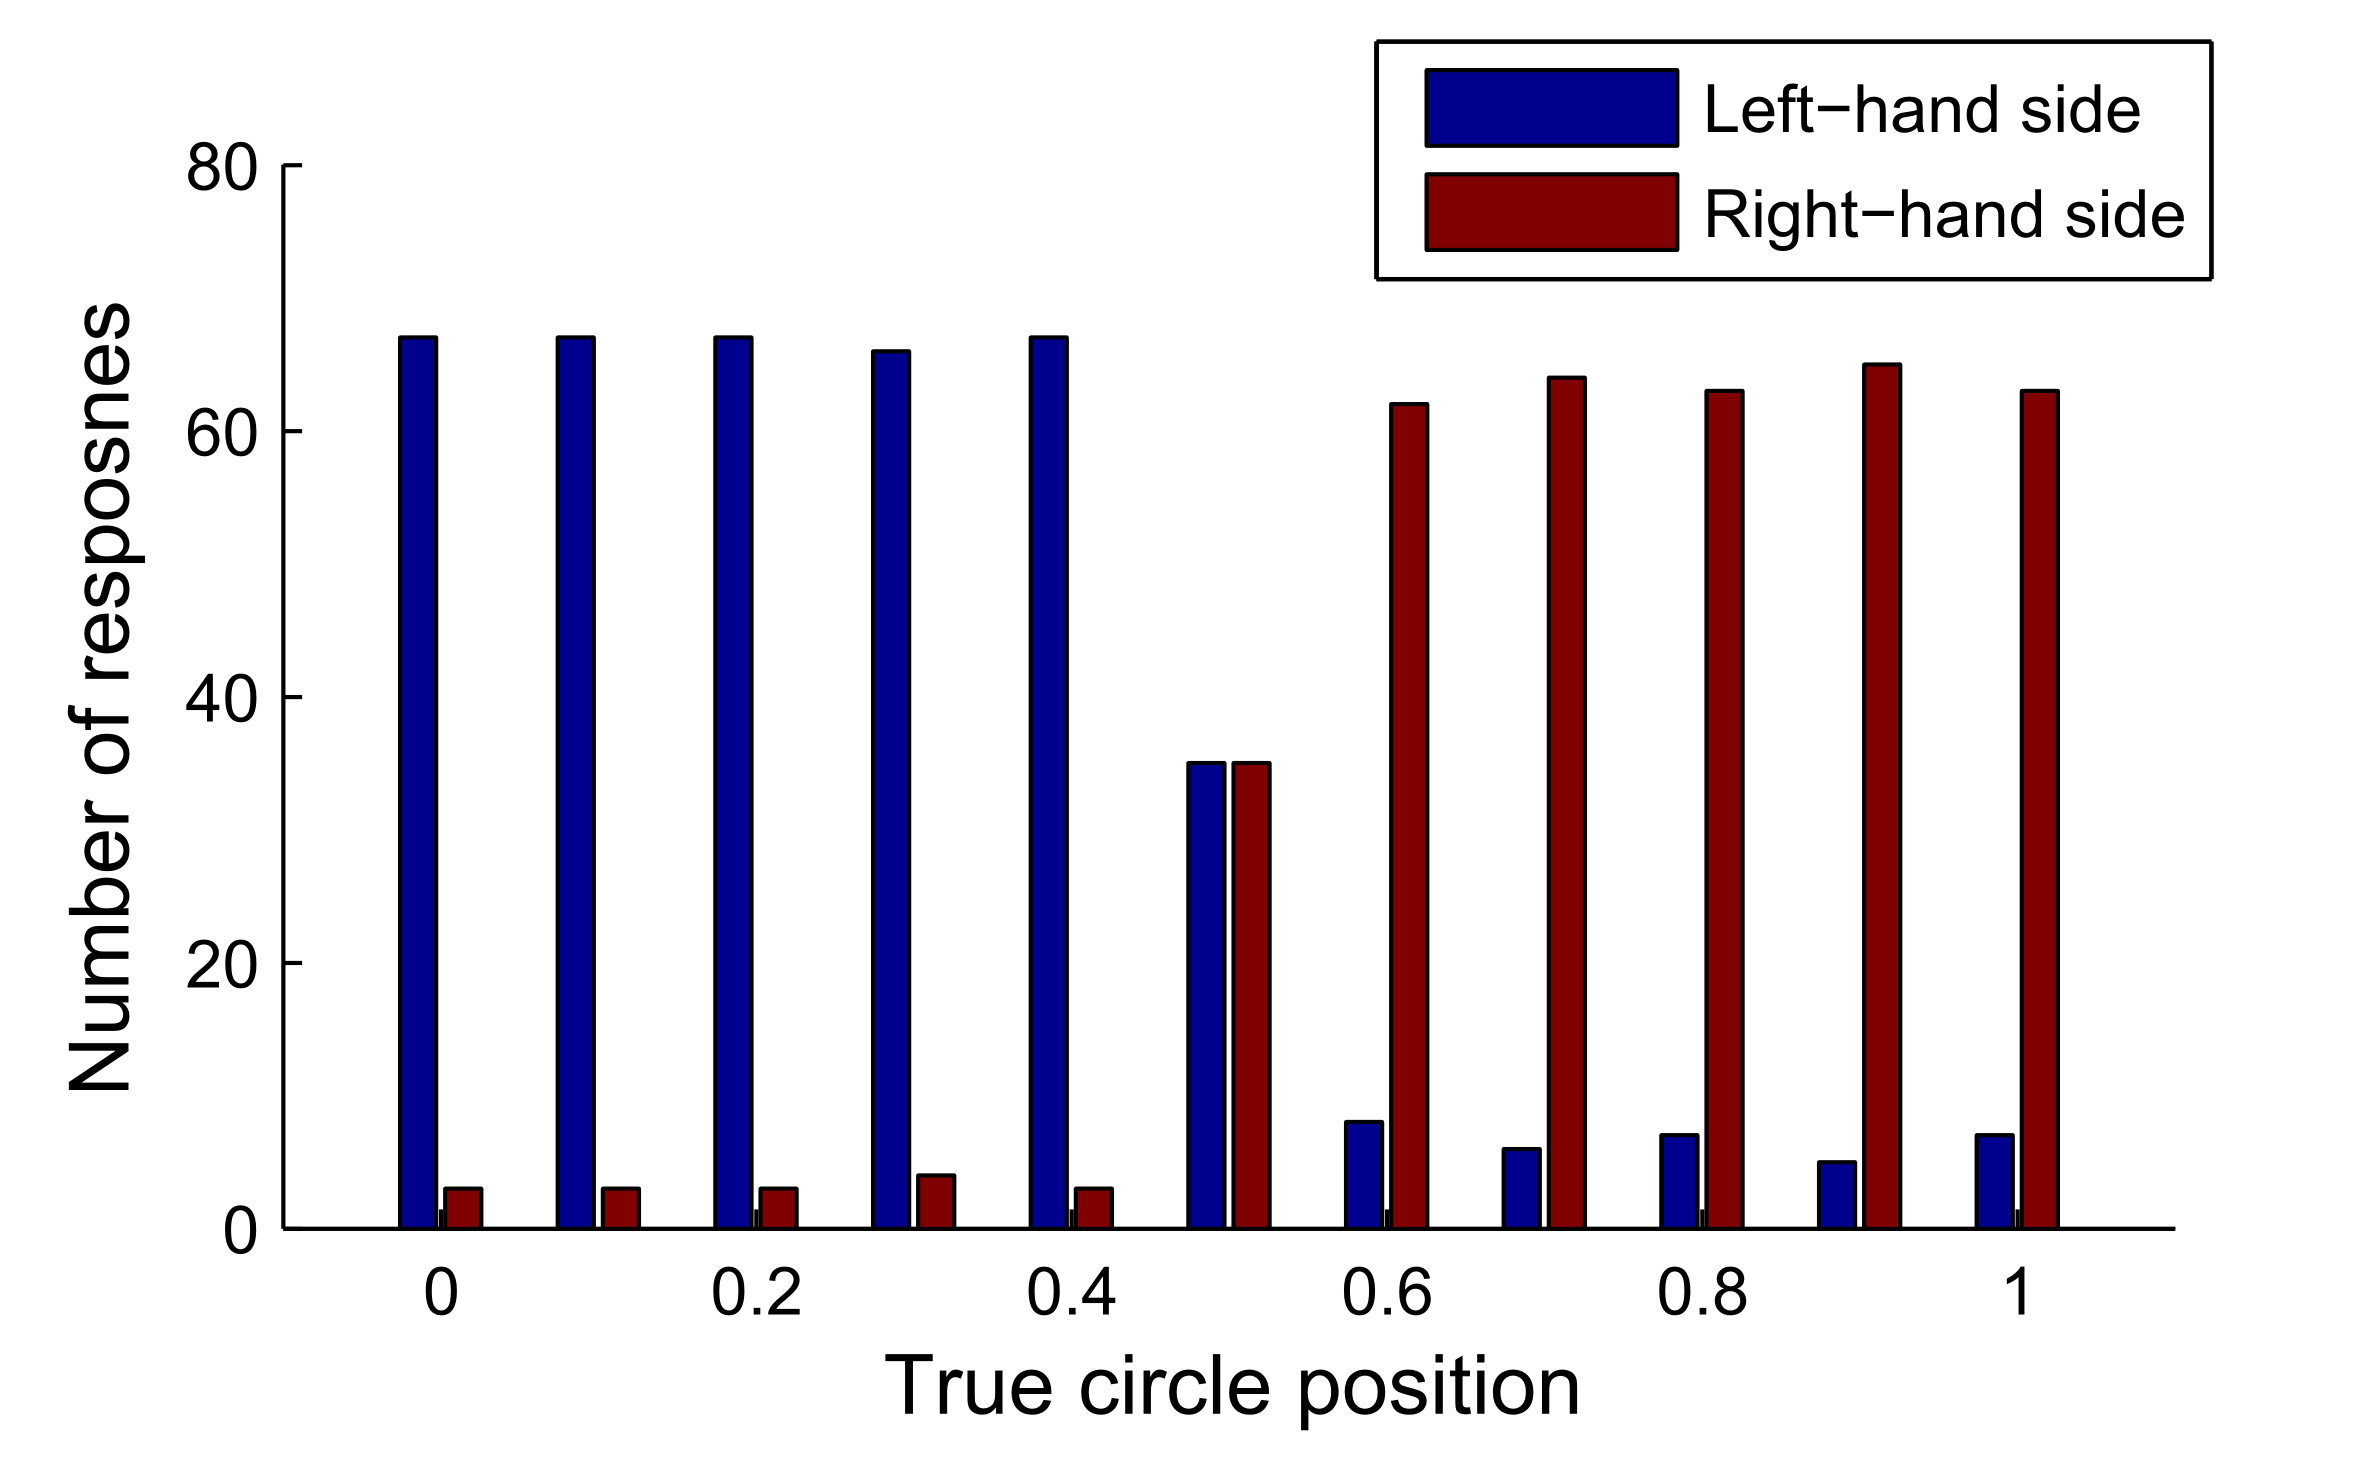
\includegraphics[scale=1]{bar_responsesLR.png}
	\caption{The number of left and right responses at each circle position. The total number of workers is 70.}
	\label{Figure:bar_responses_LR}
\end{figure}


\subsection{Non-gold responses}

We can apply  simple gold standard data filtering to the dataset. By setting the extreme values of the circle position at 0 and 1 to gold standard data, we can filter out some workers. A total of 7 workers, or 10\% of the dataset, were filtered out. \ref{Figure: not_gold_responsesLR} shows the workers that were filtered out. In \ref{Figure: line_not_gold_responseLR} we can see the response models of the individual workers. Some show the opposite from what we might expect, by responding `Left-hand side' when the circle was on the far right. This suggests that they have not understood the answer they are giving. \ref{Figure: bar_not_goldLR} shows the responses at each circle position for 


\begin{figure}
	\centering
	\begin{subfigure}{7cm}
	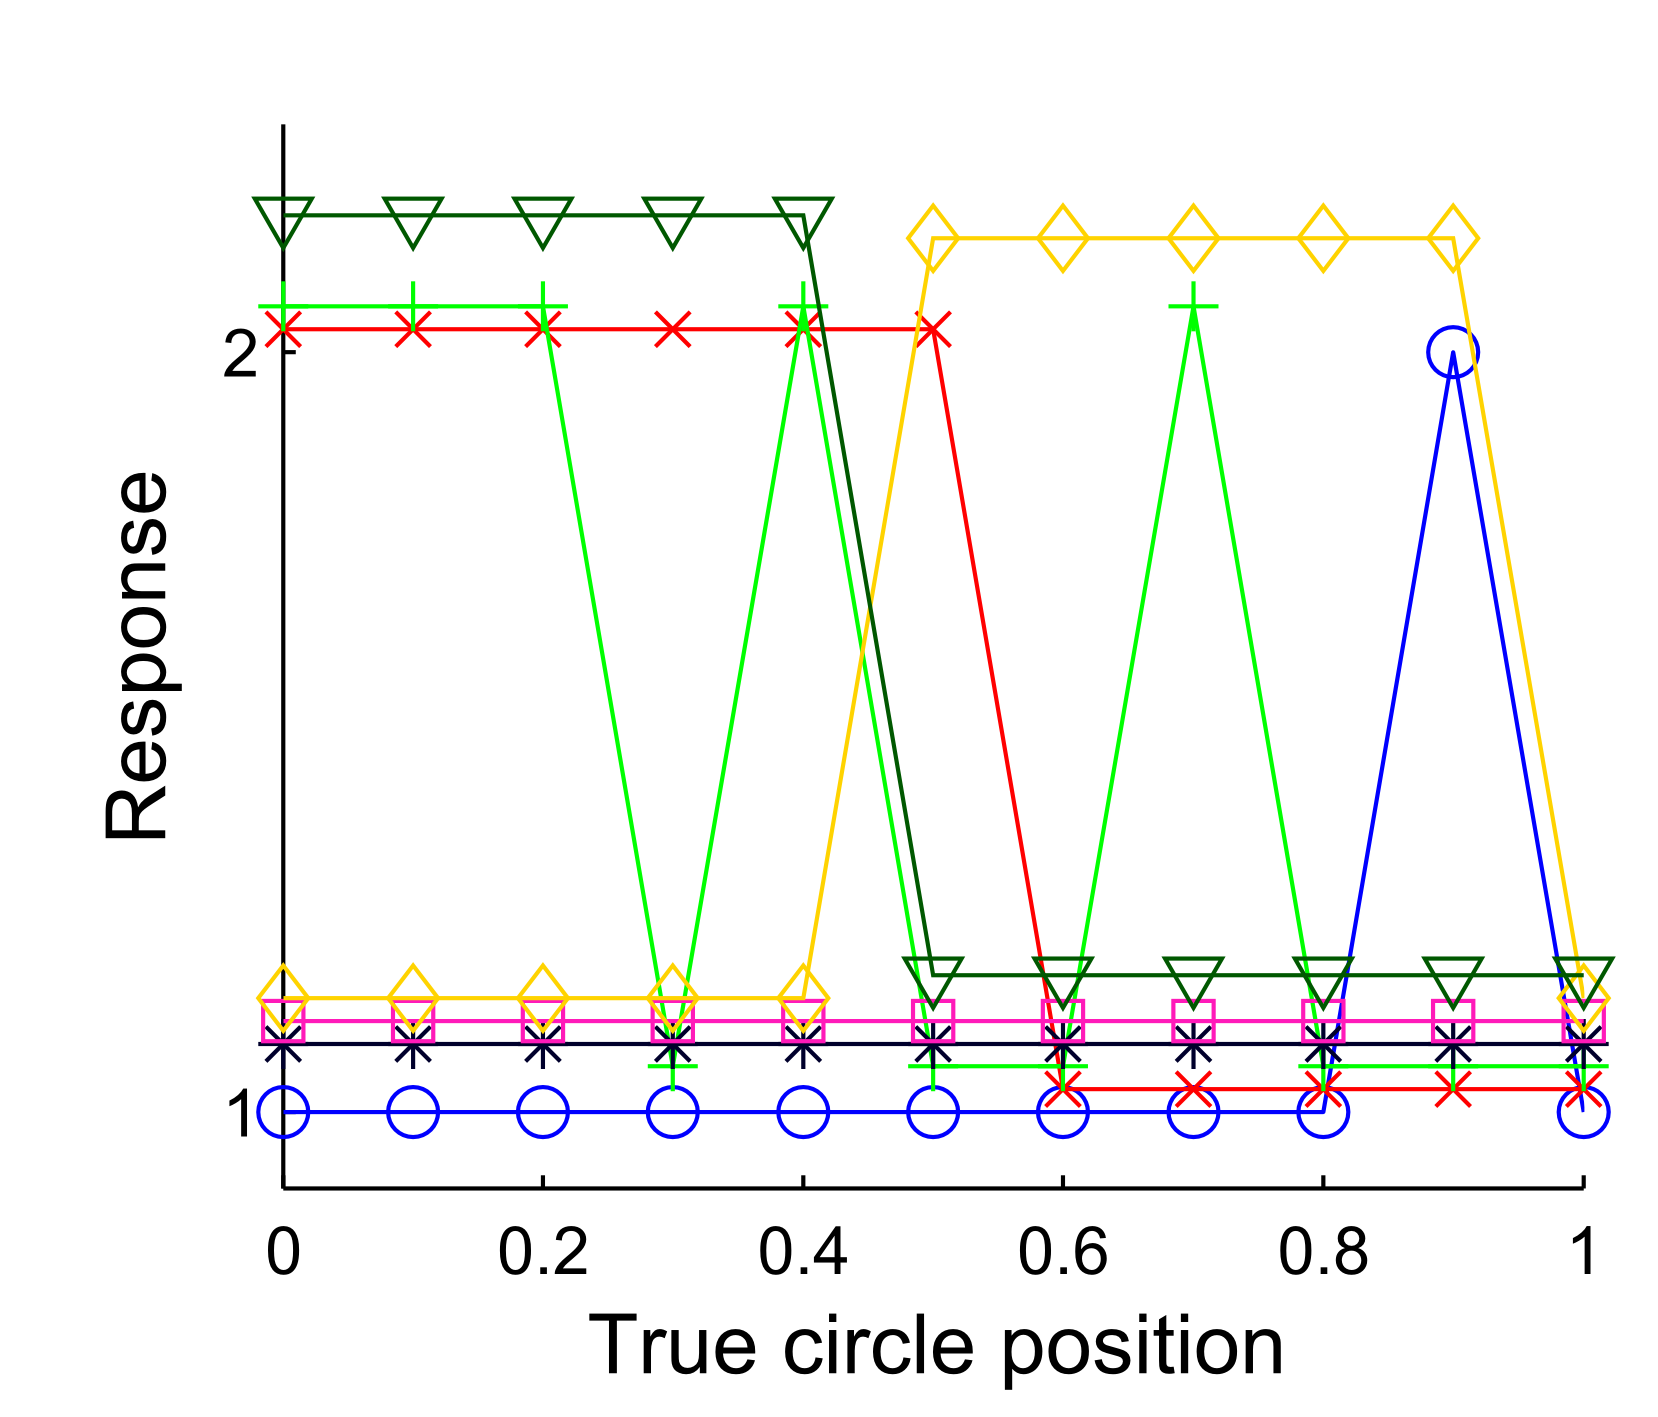
\includegraphics[scale=1]{line_not_gold_response_curves.png}
	\caption{}	
	\label{Figure: line_not_gold_responseLR}
	\end{subfigure}
	\begin{subfigure}{7cm}
	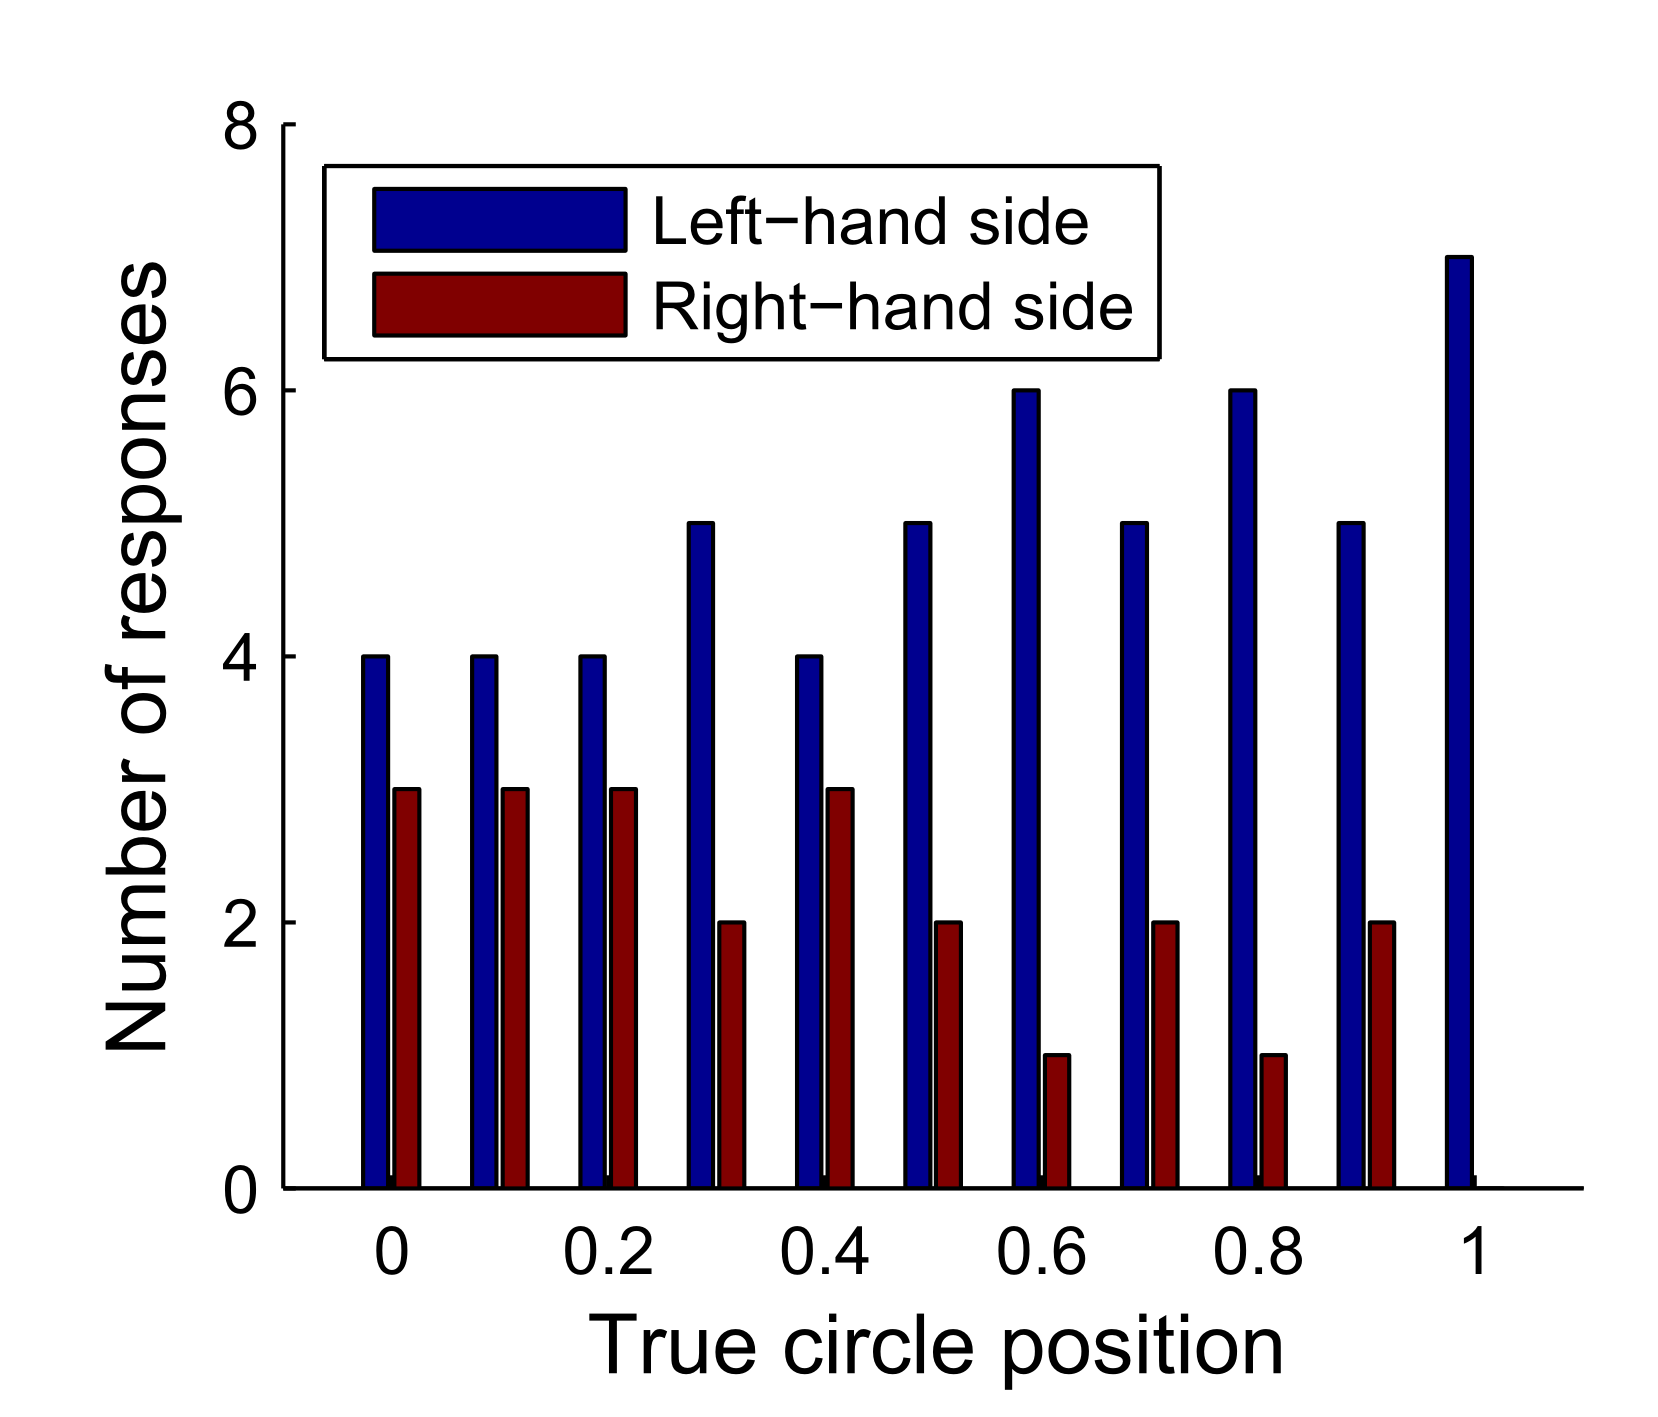
\includegraphics[scale=1]{bar_not_gold_responsesLR.png}
	\caption{}
	\label{Figure: bar_not_goldLR}	
	\end{subfigure}
	\label{Figure: not_gold_responsesLR}
	\caption{The number of left and right responses for the non-gold response workers. The total number of workers is 7.}
\end{figure}

The resulting dataset after gold filtering is shown in figure \ref{Figure:bar_gold_responsesLR}


\begin{figure}
	\centering
	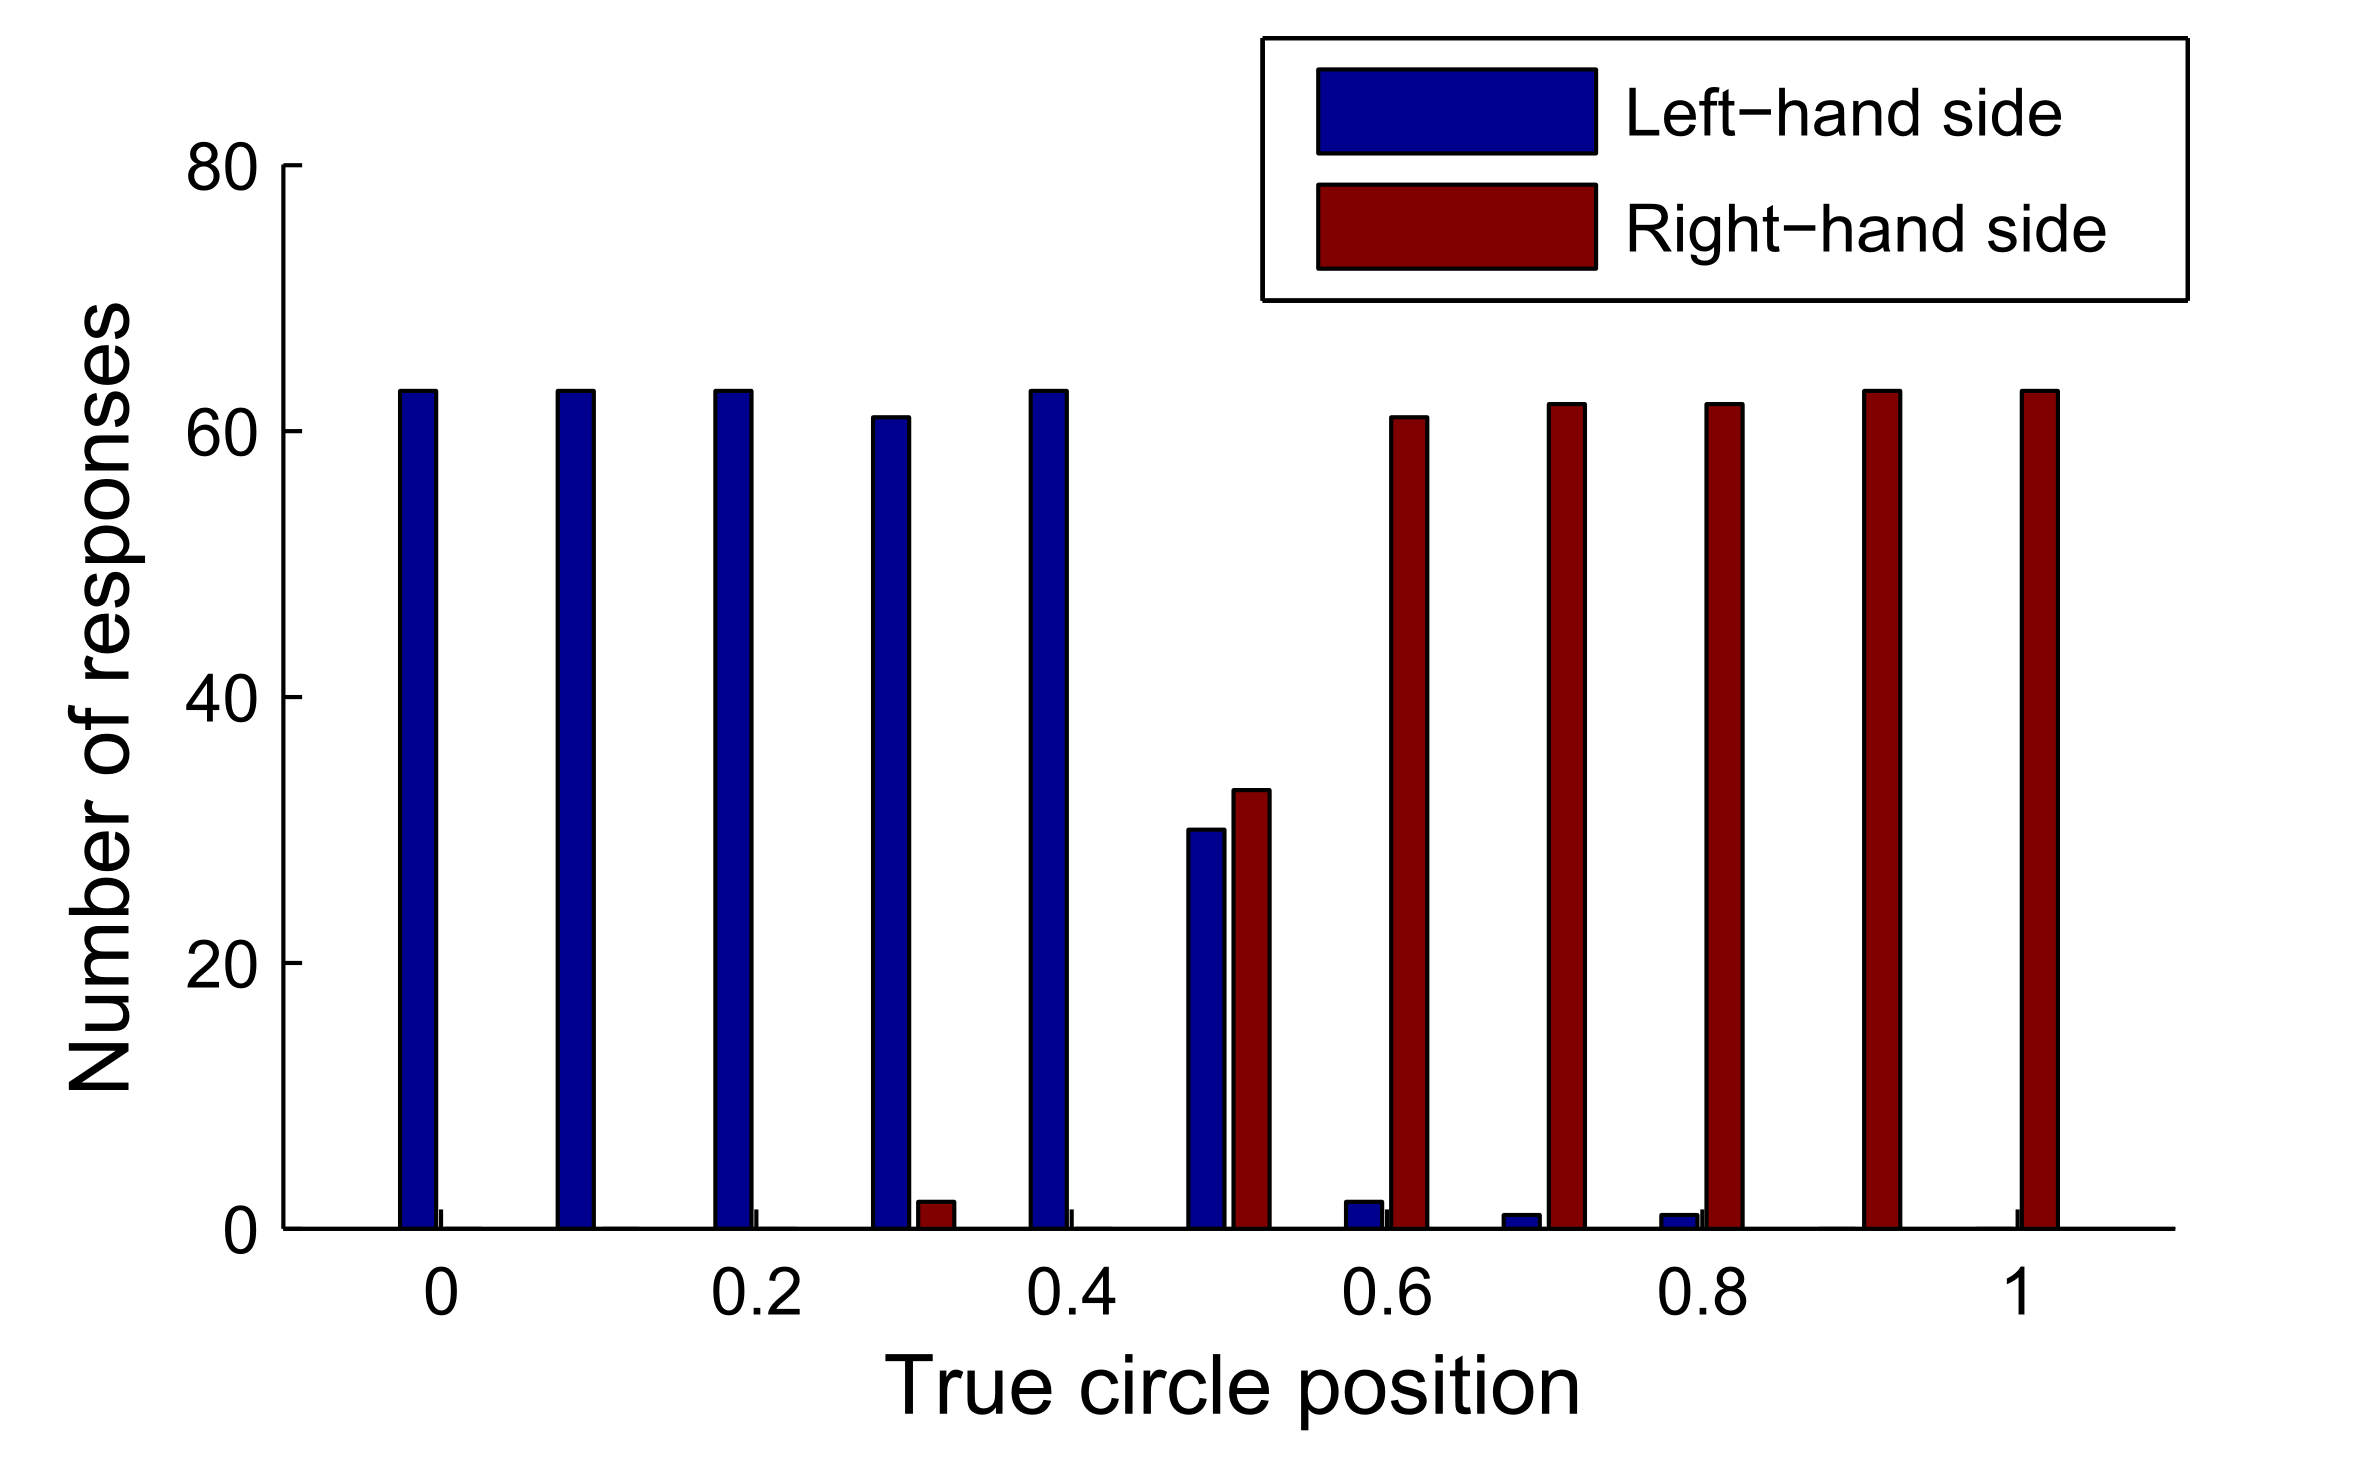
\includegraphics[scale=1]{bar_gold_responsesLR.png}
	\caption{The number of left and right responses at each circle position with gold filtering. The total number of workers is 63.}
	\label{Figure:bar_gold_responsesLR}
\end{figure}


\section{Softmax Function Fitting}

FIGURE shows the softmax function fit for the full dataset and gold standard dataset.



\section{Fusion Results}

\begin{figure}
	\centering
	\begin{subfigure}{7cm}
	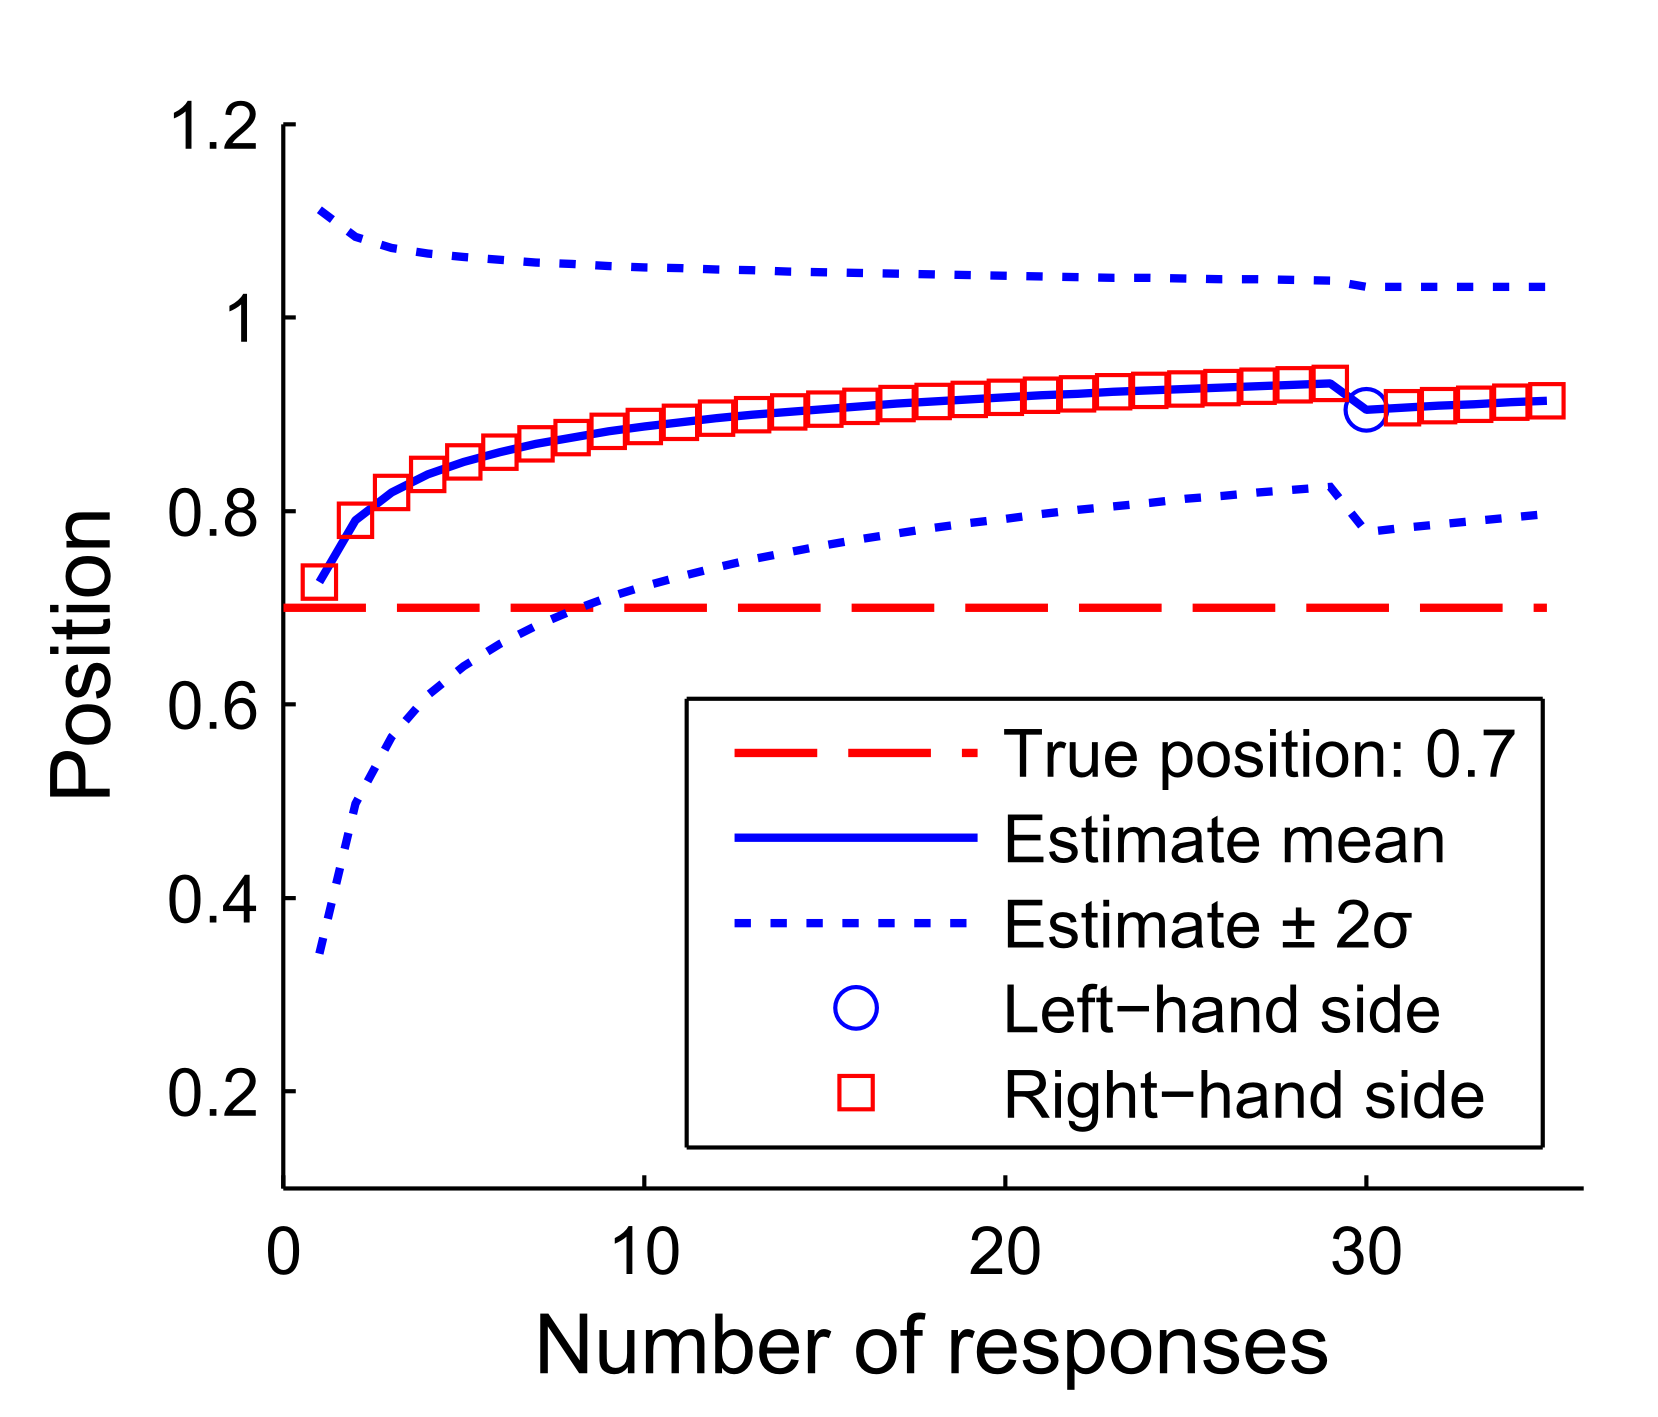
\includegraphics[scale=1]{line_fusion_responses_07_LR.png}
	\caption{}	
	\label{Figure: fusion_responses_07_varying_LR}
	\end{subfigure}
	\begin{subfigure}{7cm}
	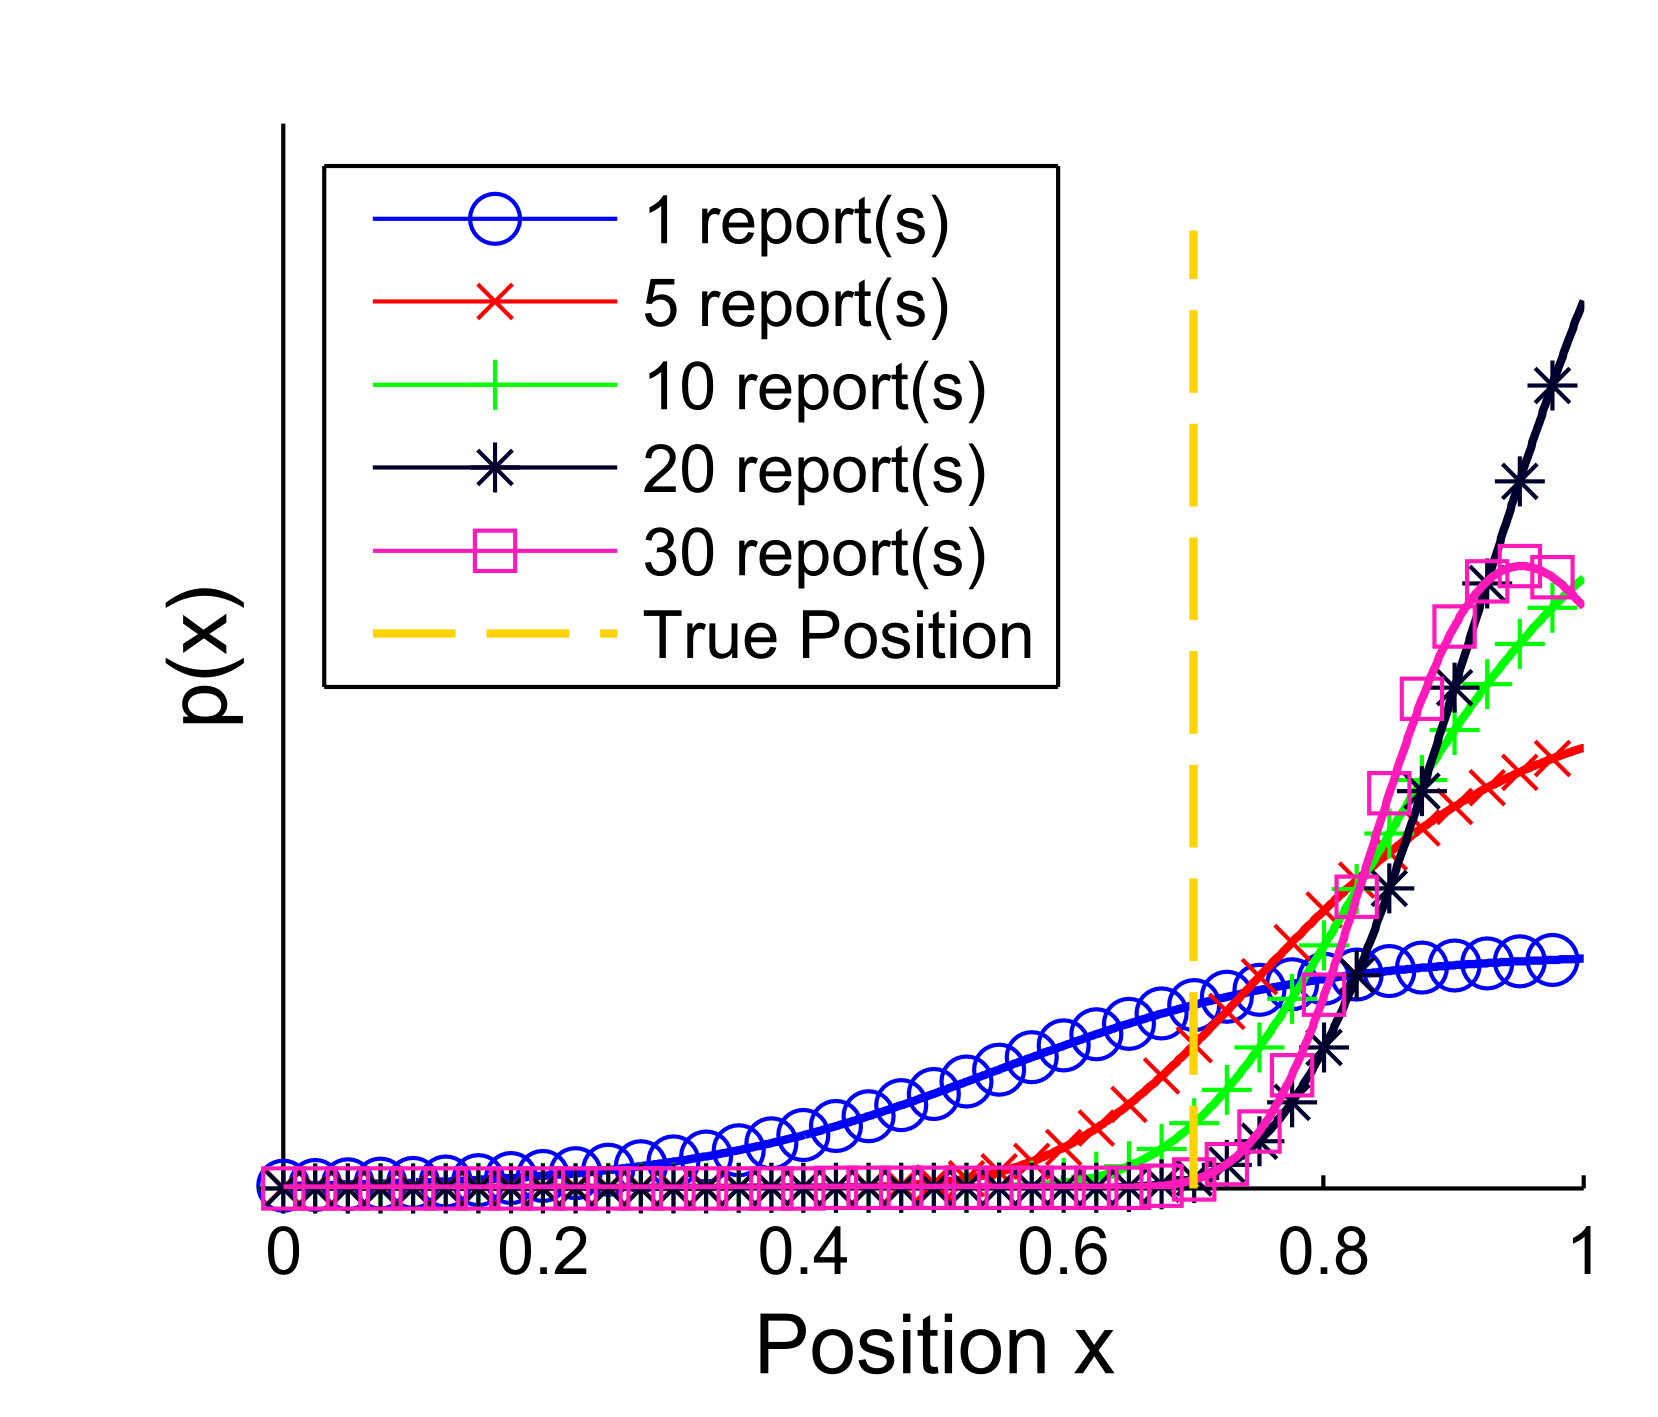
\includegraphics[scale=1]{line_fusion_07_distsLR.png}
	\caption{}
	\label{Figure: fusion_responses_07_dists_LR}	
	\end{subfigure}
	\label{Figure: fusion_responses_07_LR}
	\caption{Estimating the position of a circle as new reports are received \subref{Figure: fusion_responses_07_varying_LR}) The cahnge in posterior mean and standard deviation with responses \subref{Figure: fusion_responses_07_dists_LR}) Examples of the posterior distribution at different numbers of reports}
\end{figure}





\begin{figure}
	\centering
	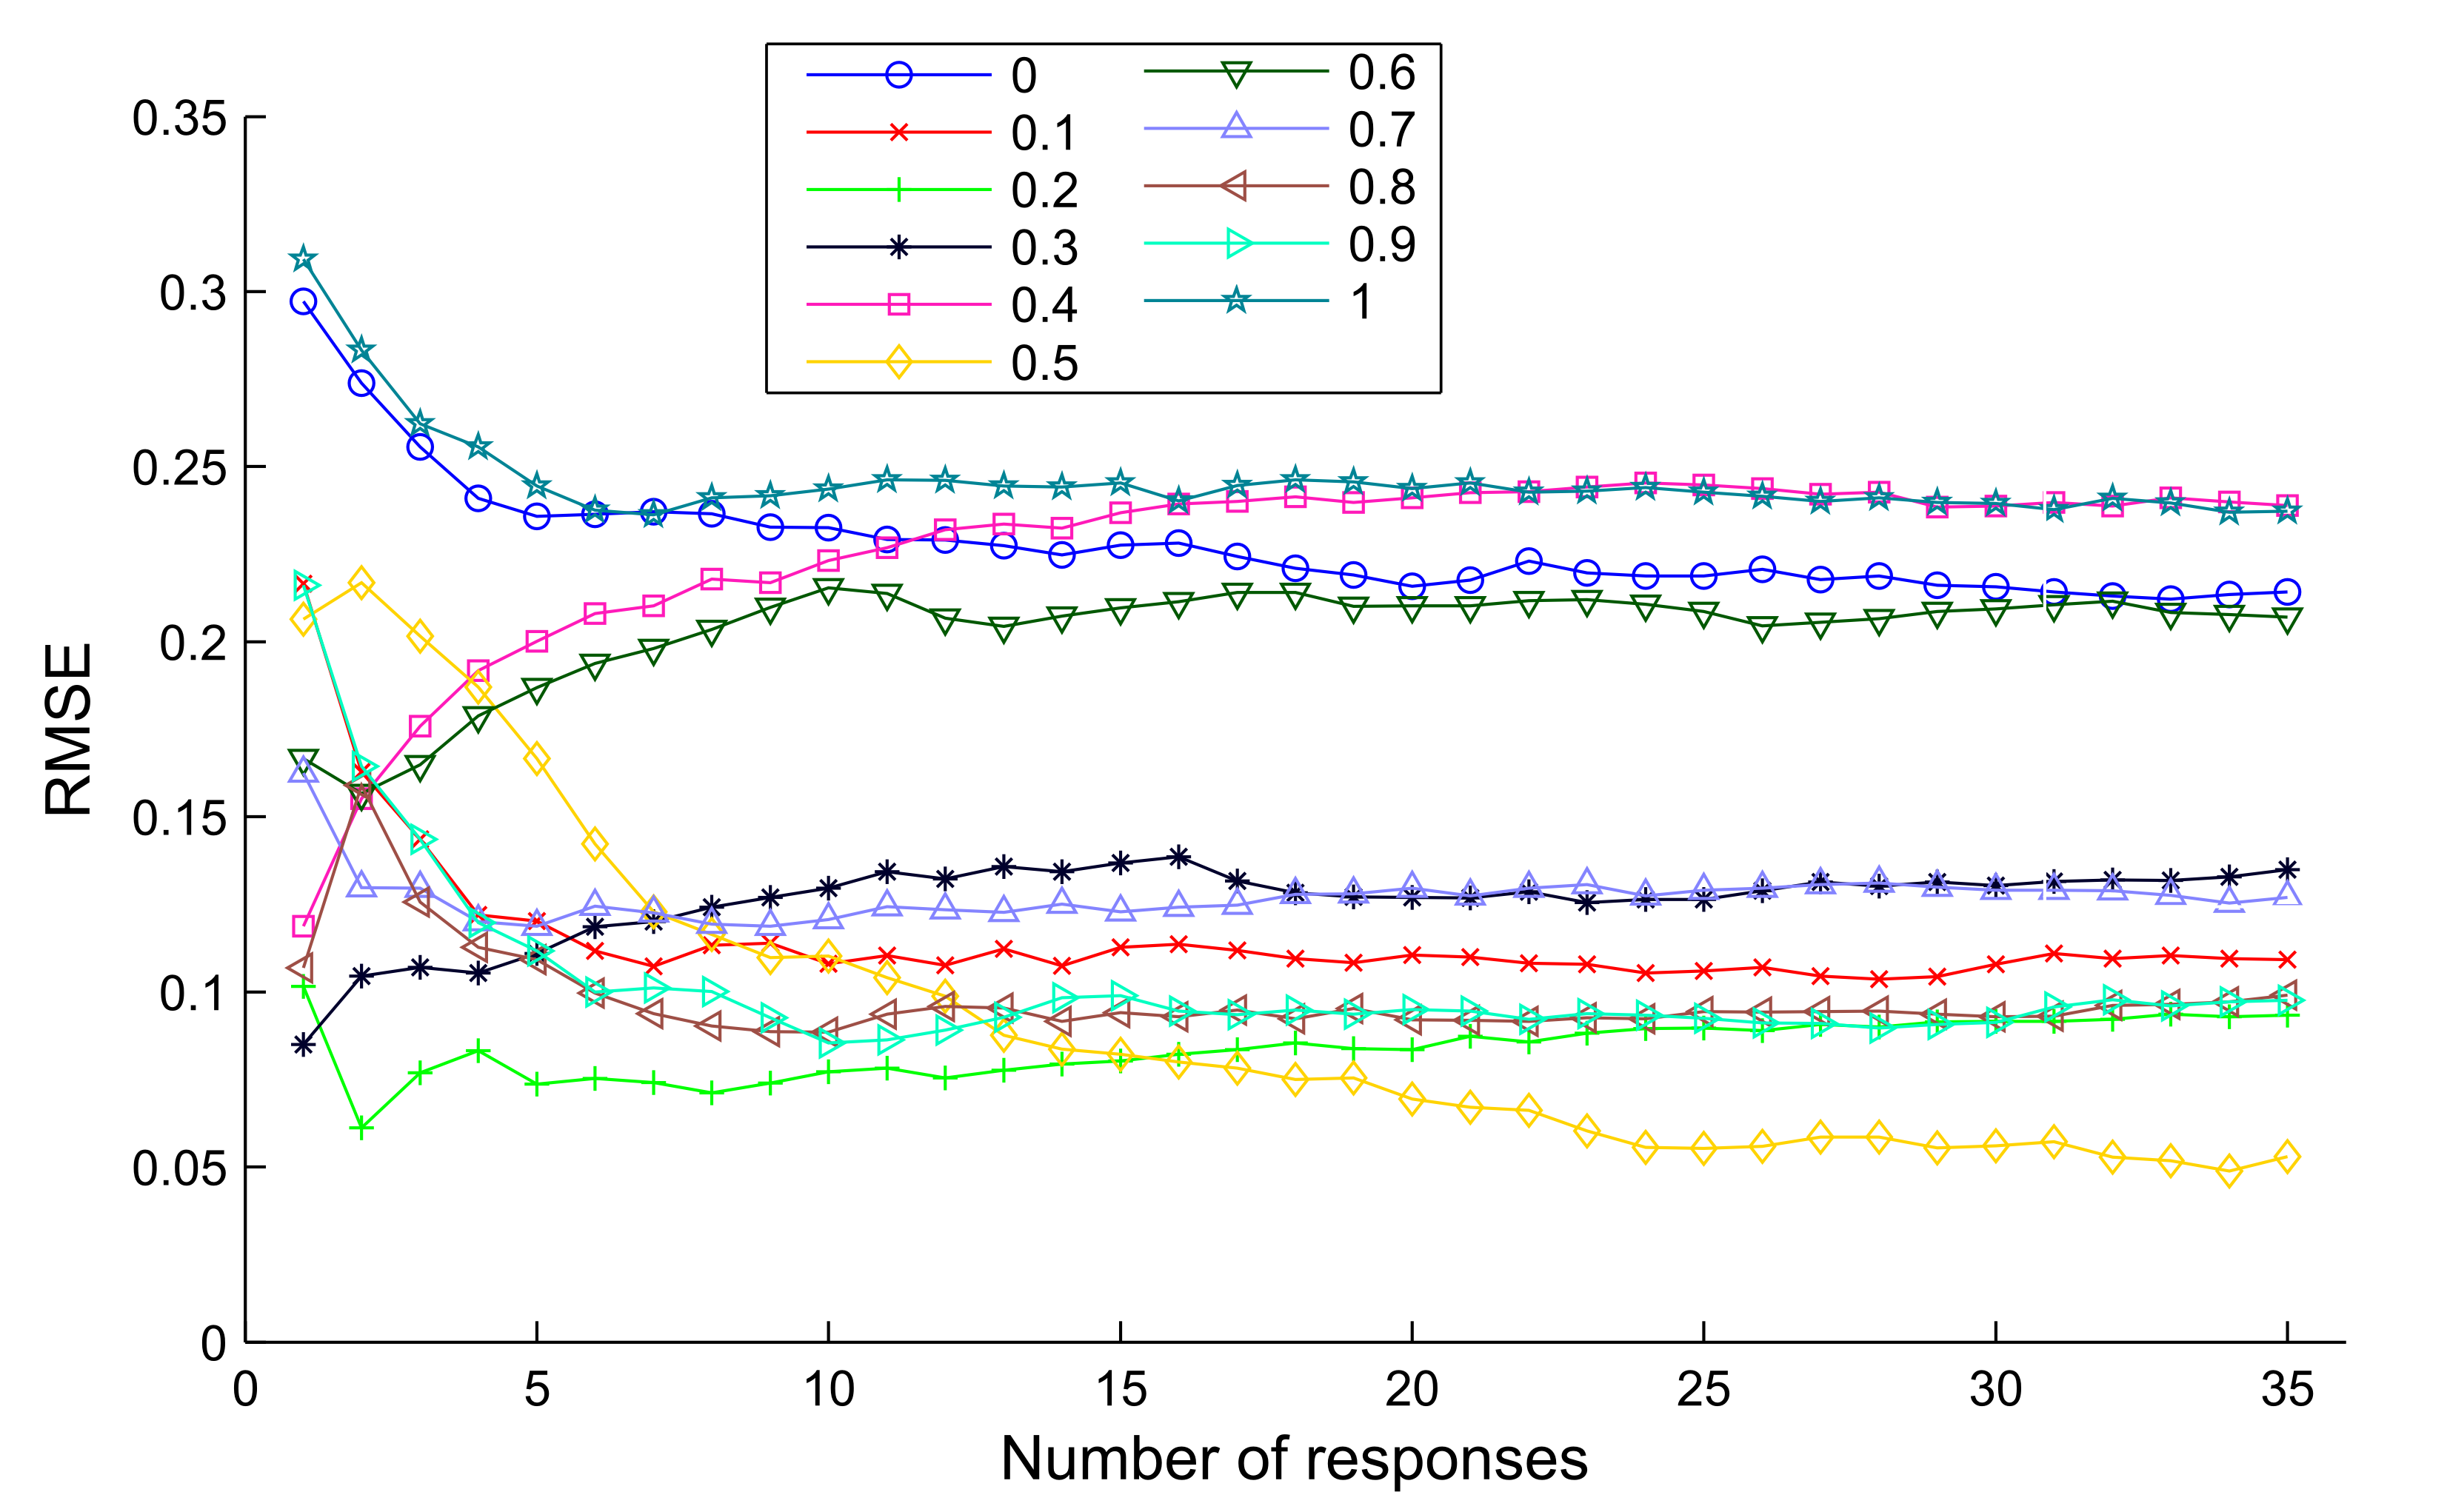
\includegraphics[scale=1]{line_fusion_RMSE_LR.png}
	\label{Figure: fusion_RMSE_LR }
	\caption{The RMSE at each circle position as the number of responses increases. The RMSE was generated over 50 simulation runs}
\end{figure}






\begin{figure}
	\centering
	\begin{subfigure}{7cm}
	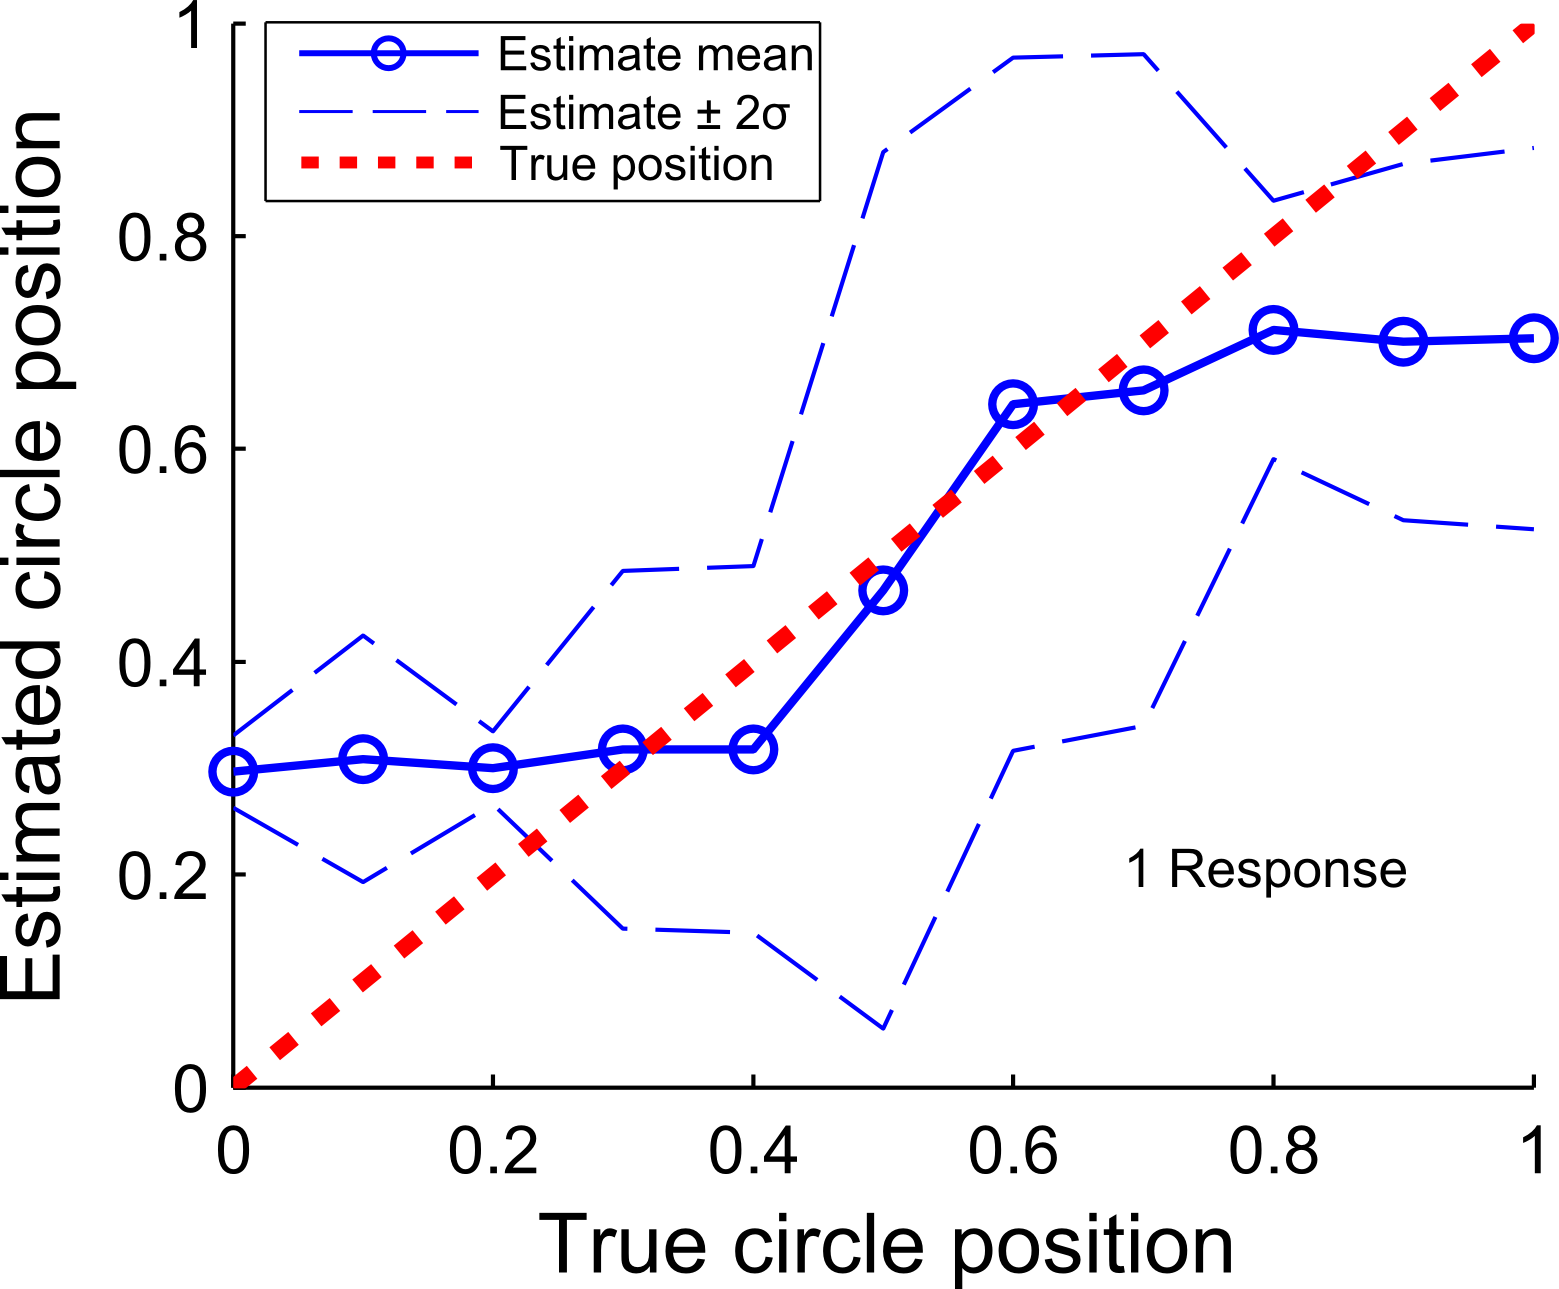
\includegraphics[scale=1]{line_fusion_mean_1rep_LR.png}
	\caption{}	
	\label{Figure: fusion_mean_1_LR}
	\end{subfigure}
	\begin{subfigure}{7cm}
	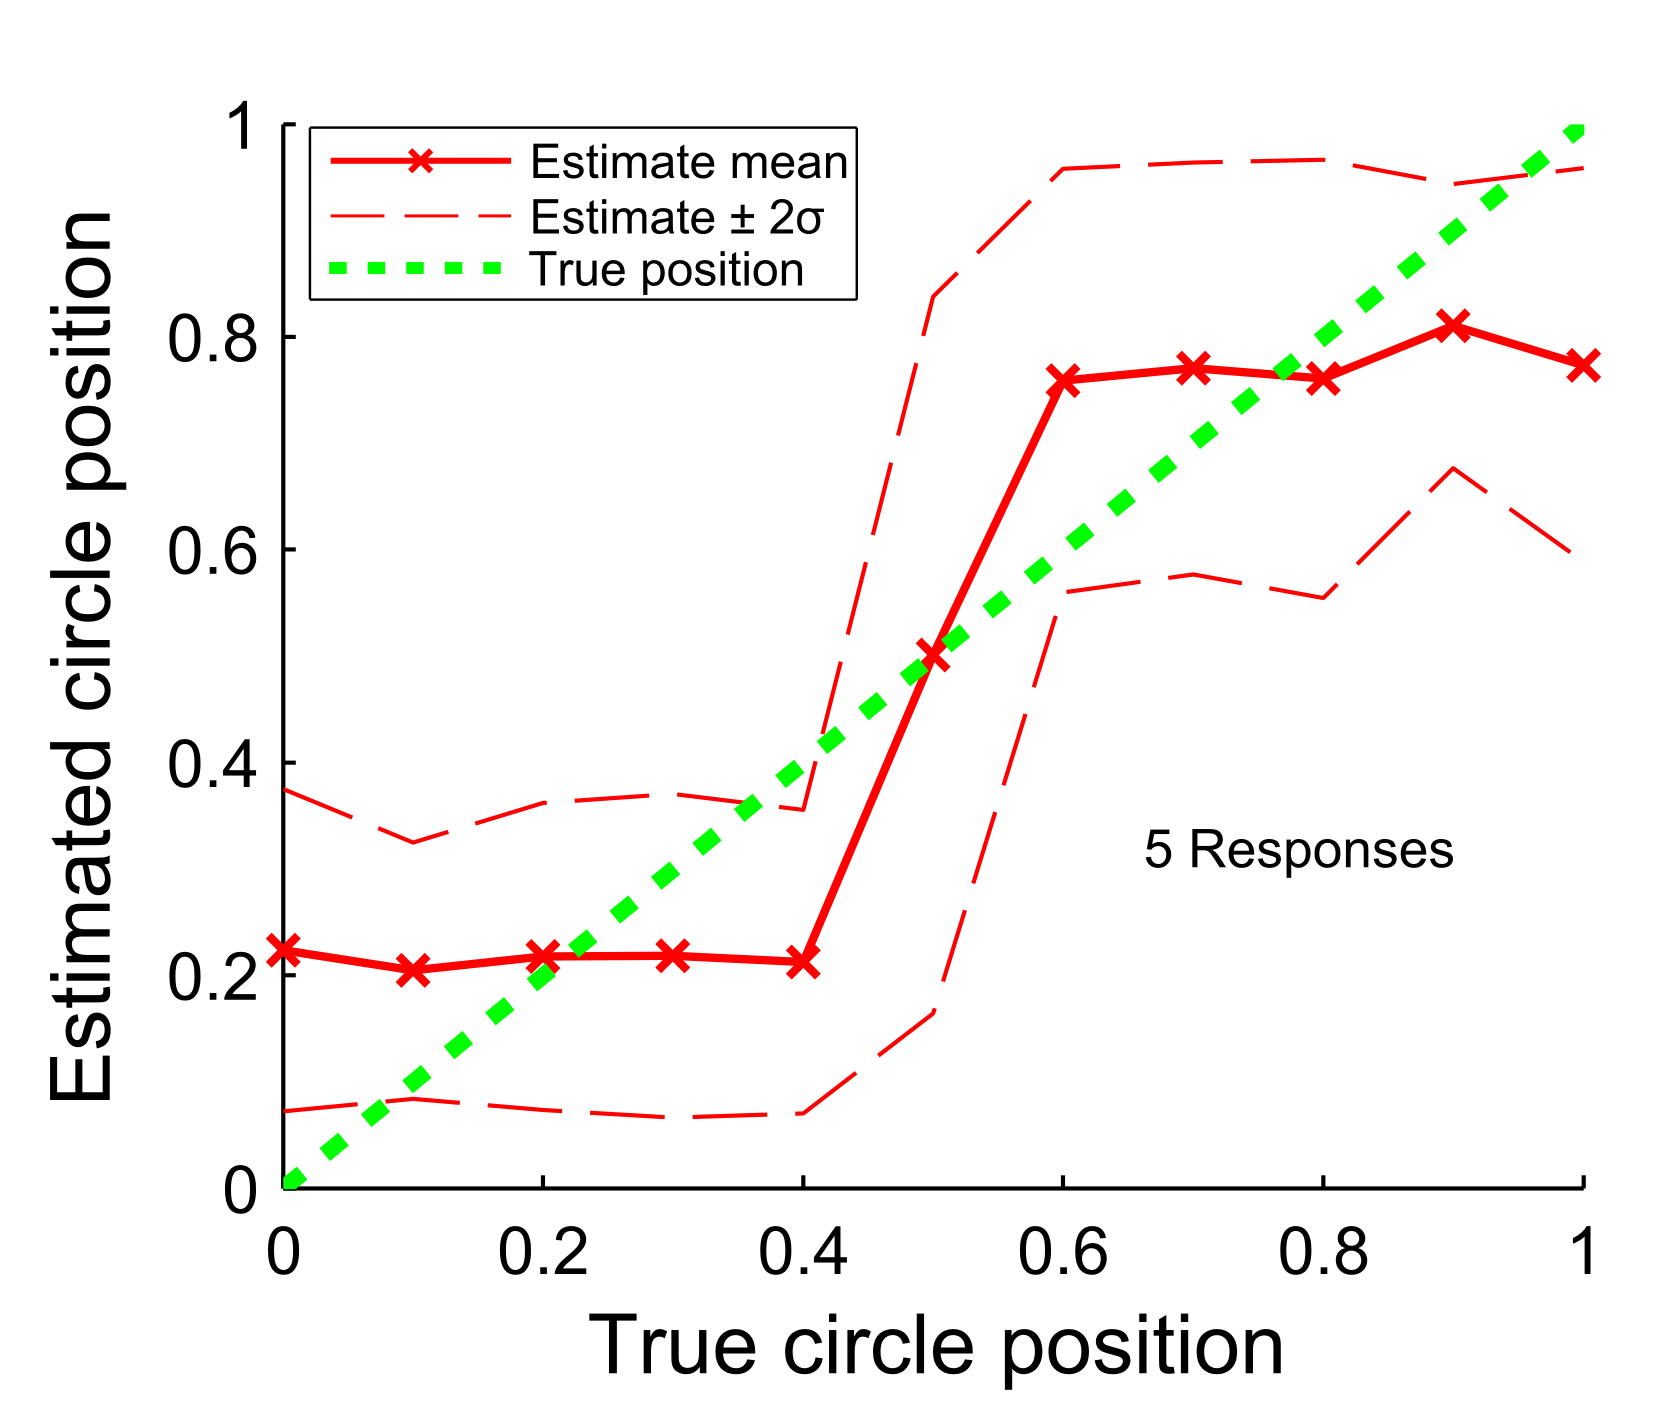
\includegraphics[scale=1]{line_fusion_5rep_LR.png}
	\caption{}
	\label{Figure: fusion_mean_5_LR}	
	\end{subfigure}\\
	\begin{subfigure}{7cm}
	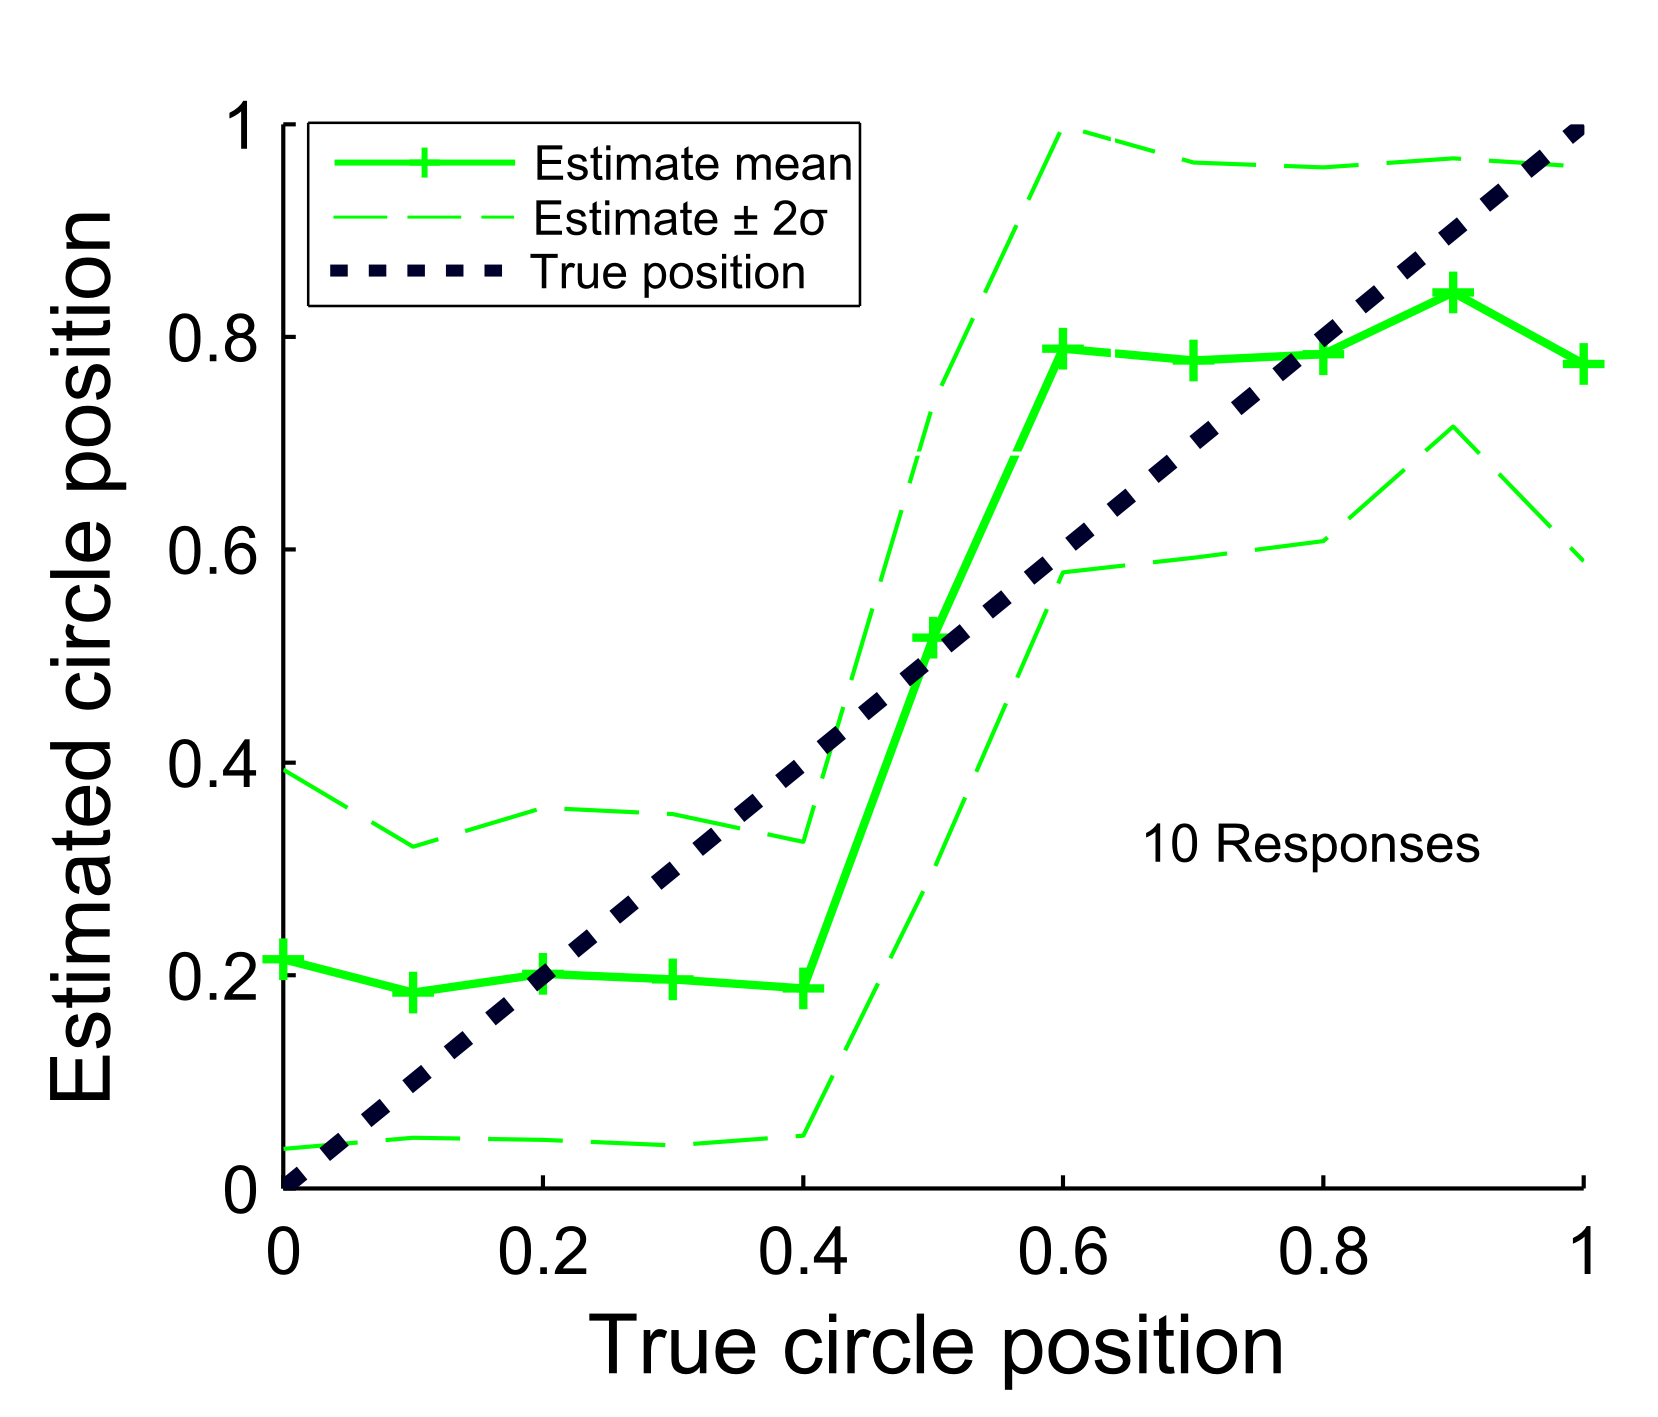
\includegraphics[scale=1]{line_fusion_10rep_LR.png}
	\caption{}	
	\label{Figure: fusion_mean_10_LR}
	\end{subfigure}
	\begin{subfigure}{7cm}
	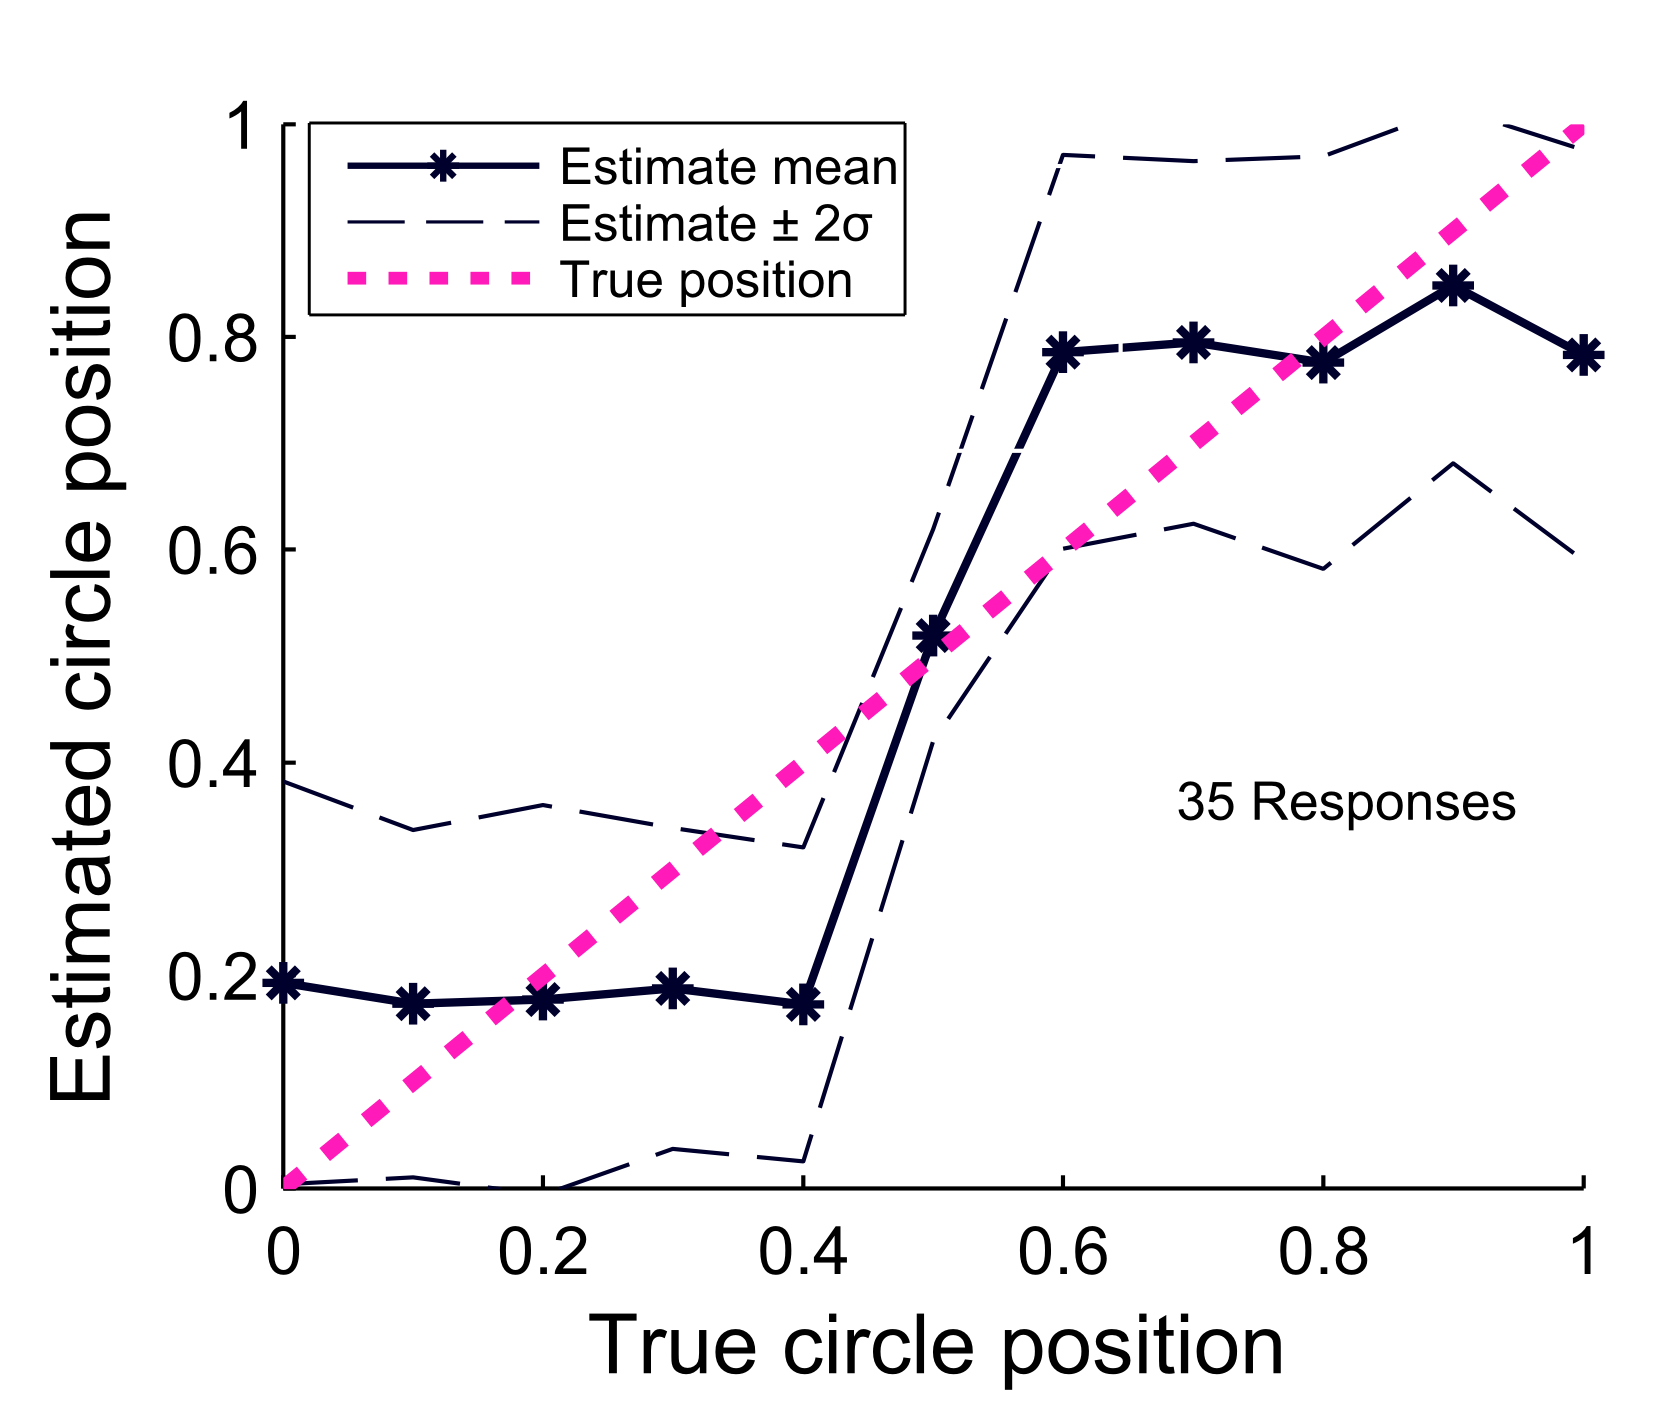
\includegraphics[scale=1]{line_fusion_35rep_LR.png}
	\caption{}	
	\label{Figure: fusion_mean_35_LR}
	\end{subfigure}
	\label{Figure: fusion_mean_LR}
	\caption{The mean performance of estimating the circle's position. The mean line is the expectation value of the posterior distribution taken from 50 simulations. The standard deviation is for the spread of expectation values over the simulations - not the spread in individual posteriors. The data was collected for varying numbers of responses with \subref{Figure: fusion_mean_1_LR}) 1 response \subref{Figure: fusion_mean_5_LR}) 5 responses \subref{Figure: fusion_mean_10_LR}) 10 responses \subref{Figure: fusion_mean_35_LR})35 responses}
\end{figure}
%\chapter{1D Positional experiments - 3 Categories} \label{Chapter: 1DPosition}

\newlength\figureheight
\newlength\figurewidth


\section{Experimental setup}
EDIT IMAGES
Crowdflower \footnote{ http://crowdflower.com/} is an online service that allows for simple tasks to be posted to a number of crowdsourcing worker markets. 
By providing a wrapper and common API for several crowdsourcing provides, Crowdflower boasts the largest crowd of workers out of any platform. 
Due to limitations in its API, only relatively simple tasks can be posted. 
Crowdflower was used to post a series of simple images to the crowd, getting feedback from hundreds of workers.

All the following experiments consisted of showing a static image of a circle to workers who were required to pick the best 1 of 2 or more avaiable options which described the location of the circle in the image. 

Each worker was shown a series of images, where the position of the circle changed from image to image, with each worker providing a single response for each image. 
A total of 11 images were shown to each worker, with the position of the circle ranging from 0 to 1 \footnote{The units are arbitrary, but the values $0:0.1:1$ are used throughout}, as shown in \ref{Figure:1d_position_images} . 
For each experiment, a simple html page was created with the images stored in a public Dropbox folder. 


% 1d circle pictures
\begin{figure}
  \centering
  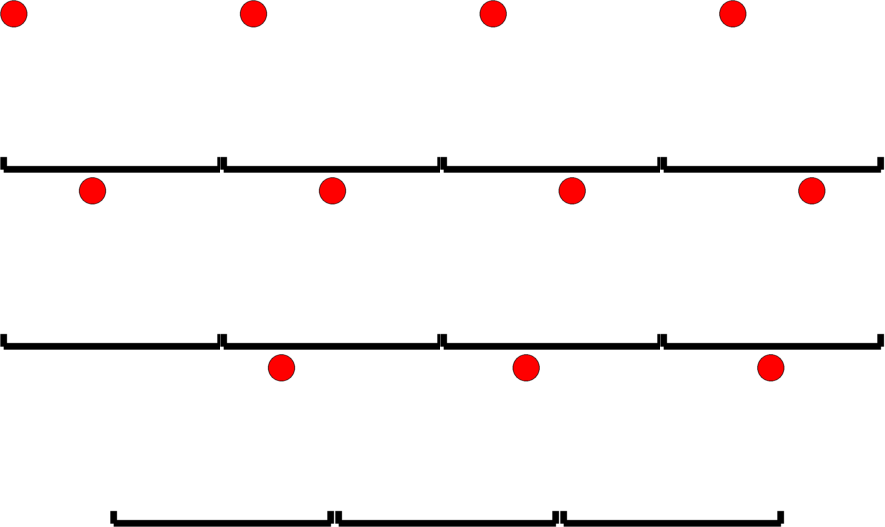
\includegraphics[width=8cm]{combined_1d_images.png}
  \caption{The images posted to the crowd. These show the circle at positions $0:0.1:1$ giving a total of 11 images }
  \label{Figure:1d_position_images}
\end{figure}

\section{3 Category Decisions}
Let \possResVec be an \nPossRes valued discrete variable that represents the possible worker responses, where $\possResVec \in \mathbb{N}$ .
Workers were asked to describe the position of the circle using one of three responses $\realPossResVec = \lbrace 'NearTheLeft', 'NearTheCentre' , 'NearTheRight'\rbrace$, which were mapped to $\possResVec=\lbrace 1,2,3 \rbrace$, setting $\nPossRes=3$.
An example of the worker GUI is shown in \ref{Figure:crowdflower_question_3} (current screenshot does not show image as dropbox is not accessible from BAE systems - get another screenshot). 
Each worker was shown a total of  11 images. 

%%worker GUI png
\begin{figure}
  \centering
  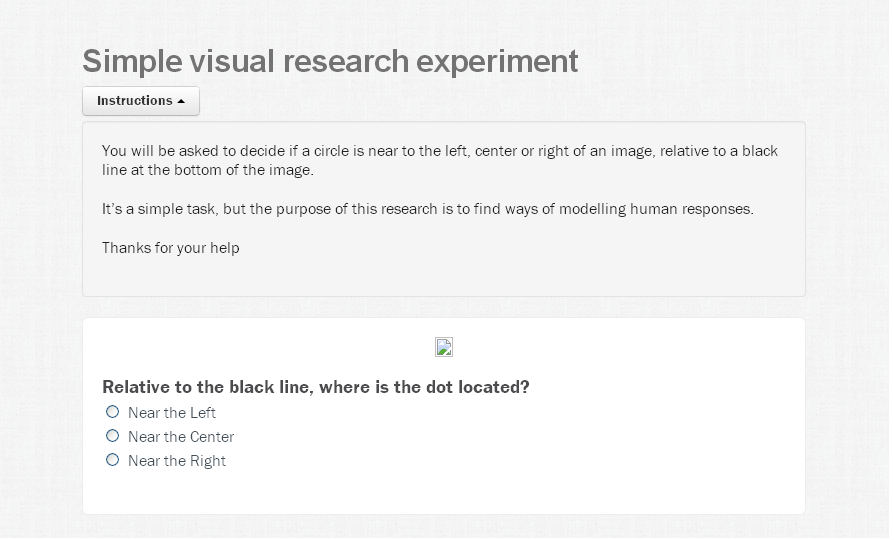
\includegraphics[width=8cm]{crowdflower_gui_noimage.png}
  \caption{The task window for a worker, requiring one of three responses}
  \label{Figure:crowdflower_question_3}
\end{figure}

A total of 100 workers were asked to provide feedback, leading to a dataset of 1100 responses. 
1 worker set, for some reason, was provided by two workers (with one worker providing 10 responses, and another 1 response), so the total number of usable workers was 99

The aim is to estimate the ground truth position of the circle given a response from 1 or more workers. 

\subsection{Dataset}

A large amount of data is returned by crowdflower, including worker responses, their declared location, their IP address, the crowdsourcing platfrom that they provided responses through, and the time each response was received. 
\tref{Table:text responses} shows a sample of three columns of the returned data which will be useful for the following analysis.


% raw table responses
\begin{table}
\centering
    \begin{tabular}{|l|l|l|}
    \hline
    \textbf{worker id} &    \textbf{image description} & \textbf{responses}       \\ \hline
    16800977      & dot located at 0.3   & Near the Left   \\
    17519077      & dot located at 0.0   & Near the Left   \\
    2666559       & dot located at 0.7   & Near the Right  \\
    16800977      & dot located at 0.5   & Near the Centre \\
    16362086      & dot located at 0.4   & Near the Centre \\ \hline
    \end{tabular}
    \caption{Example of relevant data collected}
  \label{Table:text responses}
\end{table}


In order to make analysis simpler, the strings of data in \tref{Table:text responses} were transformed in to numerical data as shown in \tref{Table:ordinal responses}.


\begin{table}
\centering
    \begin{tabular}{|l|l|l|}
    \hline
    \textbf{workers}  & \textbf{ground truth} & \textbf{responses} \\ \hline
    16800977 & 0.3          & 1         \\
    17519077 & 0.0          & 1         \\
    2666559  & 0.7          & 3         \\
    16800977 & 0.5          & 2         \\
    16362086 & 0.4          & 2         \\ \hline
    \end{tabular}
    \caption{Translation of text responses in to numerical ordinal responses }
  \label{Table:ordinal responses}
\end{table}





Let the random state variable $\possCirclePos \in \mathbb{R}$ be the circles true position. 
For this experiment the circle can take on one of $\nPossCirclePos=11$ possible positions given by $\possCirclePos = \lbrace 0.0,0.1,...,0.9,1.0 \rbrace$.
 Each worker $\workIndex$ provides a single response for each circle location. We can define the set of responses for a single worker as the vector $\workResVec_\workIndex$ where each element $\workResVec_{\workIndex,\gtIndex} \in \possResVec$, and $\workResVec_{\workIndex,\gtIndex}$ is the response of worker $\workIndex$ for true circle position $\possCirclePos_\gtIndex$



\section{Initial Analysis}

We can visualise the responses from workers as a bar chart as shown in \ref{Figure:bar responses no gold}. 
This chart shows the number of left, centre and right responses from all the workers at each of the true circle positions. 
From this chart we can see that the majority of the responses appear to be reasonable.

%Convert to PNG!
%\begin{figure}
%	\centering
%	\def\svgwidth{10cm}
%	\small
%	\import{../Figures/bar_all_responses/}{bar_all_responses.pdf_tex}
%	\caption{The number of 'NearToLeft', 'NearToRight' and 'NearToCentre' %responses at each position of the circle.}
%	\label{Figure:bar responses no gold}
%\end{figure}





\subsection{Individual Worker Response Models}

Each worker provides a single response at each true circle position. 
We can create a \textit{ response model} for each worker which simply describes that workers response at each position. 
A model for an individual is given by the workers response vector $\workResVec_\workIndex$. 
An example of a response model is shown in \ref{Figure:one worker model}

%convert to png!
%\begin{figure}
%	\centering
%	\def\svgwidth{10cm}
%	\small
%	\import{../Figures/line_single_response_curve/}%{line_single_response_curve.pdf_tex}
%	\caption{Response model for a single worker}
%	\label{Figure:one worker model}
%\end{figure}

\subsubsection{Unique Response Model Groups}
Workers can be grouped by their respective models. 
Each group is formed by workers who have identical response models i.e. at every true circle position $\possCirclePos_\gtIndex$, they reported the same position category. 
By grouping workers together, we are able to see the number of different response models there are. 
The top three most common response models are shown in \ref{Figure:top worker response models}. 
There was found to be 24 unique response model groups, 10 of which had more than 1 worker with that model, as shown in \ref{Figure:bar unique response model groups}

%\begin{figure}
%	\centering
%	\def\svgwidth{10cm}
%	\small
%	\import{../Figures/line_top_5_response_curves/}{line_top_5_response_curves.pdf_tex}
%	\caption{The top 5 unique response models}
%	\label{Figure:top worker response models}
%\end{figure}

%\begin{figure}
%	\centering
%	\def\svgwidth{10cm}
%	\small
%	\import{../Figures/bar_number_of_workers_per_group/}{bar_number_of_workers_per_group.pdf_tex}
%	\caption{The number of workers in each unique response model group}
%	\label{Figure:bar unique response model groups}
%\end{figure}

\subsubsection{Model Consistency}
We can define a response model as consistent if the difference between adjacent values in a workers response vector are always $\geqslant 0$, or $\leqslant 0$. 
We can define the response change, the change between adjacent values in a workers response vector $\workResVec_\workIndex$, as
\[\resChange=\workResVec_{\workIndex,\gtIndexCons+1}-\workResVec_{\workIndex,\gtIndexCons}\]
where $\gtIndexCons=\lbrace 1,2,...,\nPossCirclePos -1 \rbrace $

We can define three types of consistent model 

\[
\modType=
\begin{cases}
\consInc & \text{if } \forall \gtIndex, \resChange \geq 0 \text{ and } >0 \text{ for some \workIndex} \\
\consDec      & \text{if } \forall \gtIndex, \resChange \leq 0 \text{ and } < 0 \text{ for some \workIndex}\\
\consCon    & \text{if } \forall \gtIndex, \resChange = 0 
 \end{cases}
\]

where \consInc are increasing models, \consDec are decreasing models and \consCon are constant models. 
We expect the majority of consistent models to be increasing models, as the true position of the circle increases from left to right for each element of $\workResVec_\workIndex$. 
A constant consistent model represents a worker who supplied the same response no matter what the circles position. 
This points towards a worker who either did not understand the question, or more likely did not attempt the question at all - they simply filled in the submission form as quickly as possible. 
A consistent decreasing model would imply a user who either did not understand the question, or someone who is intentionally providing poor responses.
\ref{Figure:increasing worker models} shows all the increasing response models. The number of workers with each increasing response model is shown in \ref{Figure:bar increasing models}

%\begin{figure}
%	\centering
%	\begin{subfigure}{7cm}
%	\def\svgwidth{7cm}
%	\small
%	\import{../Figures/line_all_consistent_increasing/}%{line_all_consistent_increasing.pdf_tex}
%	\caption{}
%	\label{Figure:increasing worker models}
%	\end{subfigure}
%	\begin{subfigure}{7cm}
%	\def\svgwidth{7cm}
%	\small
%	\import{../Figures/bar_consistent_increasing/}{bar_consistent_increasing.pdf_tex}
%	\caption{}
%	\label{Figure:bar increasing models}
%	\end{subfigure}
%	\caption{Increasing consistent response models \subref{Figure:increasing worker models}) All the unique models with increasing response consistency \subref{Figure:bar increasing models}) The number of workers with each increasing model }
%\end{figure}





\subsubsection{Model Symmetry}
Some of the models showed \textit{symmetry},(Is it symmetry? How do we define it?). Let $f_{s}(\workResVec)$
be a function which transforms a workers response vector, so that each 1 is transformed to 3, and a 3 is transformed to 1. Two types of symmetry can be defined


\[
\modType=
\begin{cases}

\resSym & \text{if } \forall \gtIndex, f_{s}(\workResVec_{\workIndex,\gtIndex})=\workResVec_{\workIndex,(\nPossCirclePos+1-\gtIndex)} \text{ and }\workResVec_{\workIndex,\gtIndex}\neq\workResVec_{\workIndex,(\nPossCirclePos+1-\gtIndex)} \text{ for some } \gtIndex  \\

\trueSym      & \text{if } \forall \gtIndex, \workResVec_{\workIndex,\gtIndex}=\workResVec_{\workIndex,(\nPossCirclePos+1-\gtIndex)}\\ 
 \end{cases}
\]

where \resSym is response symmetry, and \trueSym is true symmetry. 
A model has true symmetry if, at locations $0.5 + a$ and $0.5 - a$ the worker gives the same response. 
This is an undesirable type of model, as it means that using only this type of model, we would be unable to distinguish between positions such as 0.4 and 0.6.

Response symmetry is where at locations $0.5 + a$ and $0.5-a$, a worker gives the \textit{opposite} response. 
For example, if they responded 'NearTheRight' at $0.3$, they would responded 'NearTheLeft' at position $0.7$. 
A response symmetric model looks the same when rotated through $180^\circ$. 
A worker who responds only 'NearTheCentre' for every true position of the circle is defined to have a model type \trueSym. \ref{Figure:symmetry models} shows the symmetric models.
The majority of symmetric models are of the type \resSym

%\begin{figure}
%	\centering
%	\begin{subfigure}{7cm}
%	\def\svgwidth{7cm}
%	\small
%	\import{../Figures/line_true_symmetric_models/}{line_true_symmetric_models.pdf_tex}
%	\caption{}
%	\label{Figure:true symmetric models}
%	\end{subfigure}
%	\begin{subfigure}{7cm}
%	\def\svgwidth{7cm}
%	\small
%	\import{../Figures/line_response_symmetric_models/}{line_response_symmetric_models.pdf_tex}
%	\caption{}
%	\label{Figure:response symmetric models}
%	\end{subfigure}
%	\caption{Symmetric models \subref{Figure:true symmetric models}) True symmetric models \subref{Figure:response symmetric models}) Response symmetric models }
%\end{figure}


\subsection{Time Analysis}

Other than the responses of each worker, the start and finish time of each worker was available. 
This data only tells us when each worker began the task, and when she finished it - it does not tell us the amount of time they spent on each response.

FIGURE shows the average response time for each worker. 
The average response time is simply given by 

\[ 
\text{Average response time} = \frac{\text{Total task time}}{\text{Number of responses}}
\]

\begin{figure}
\centering
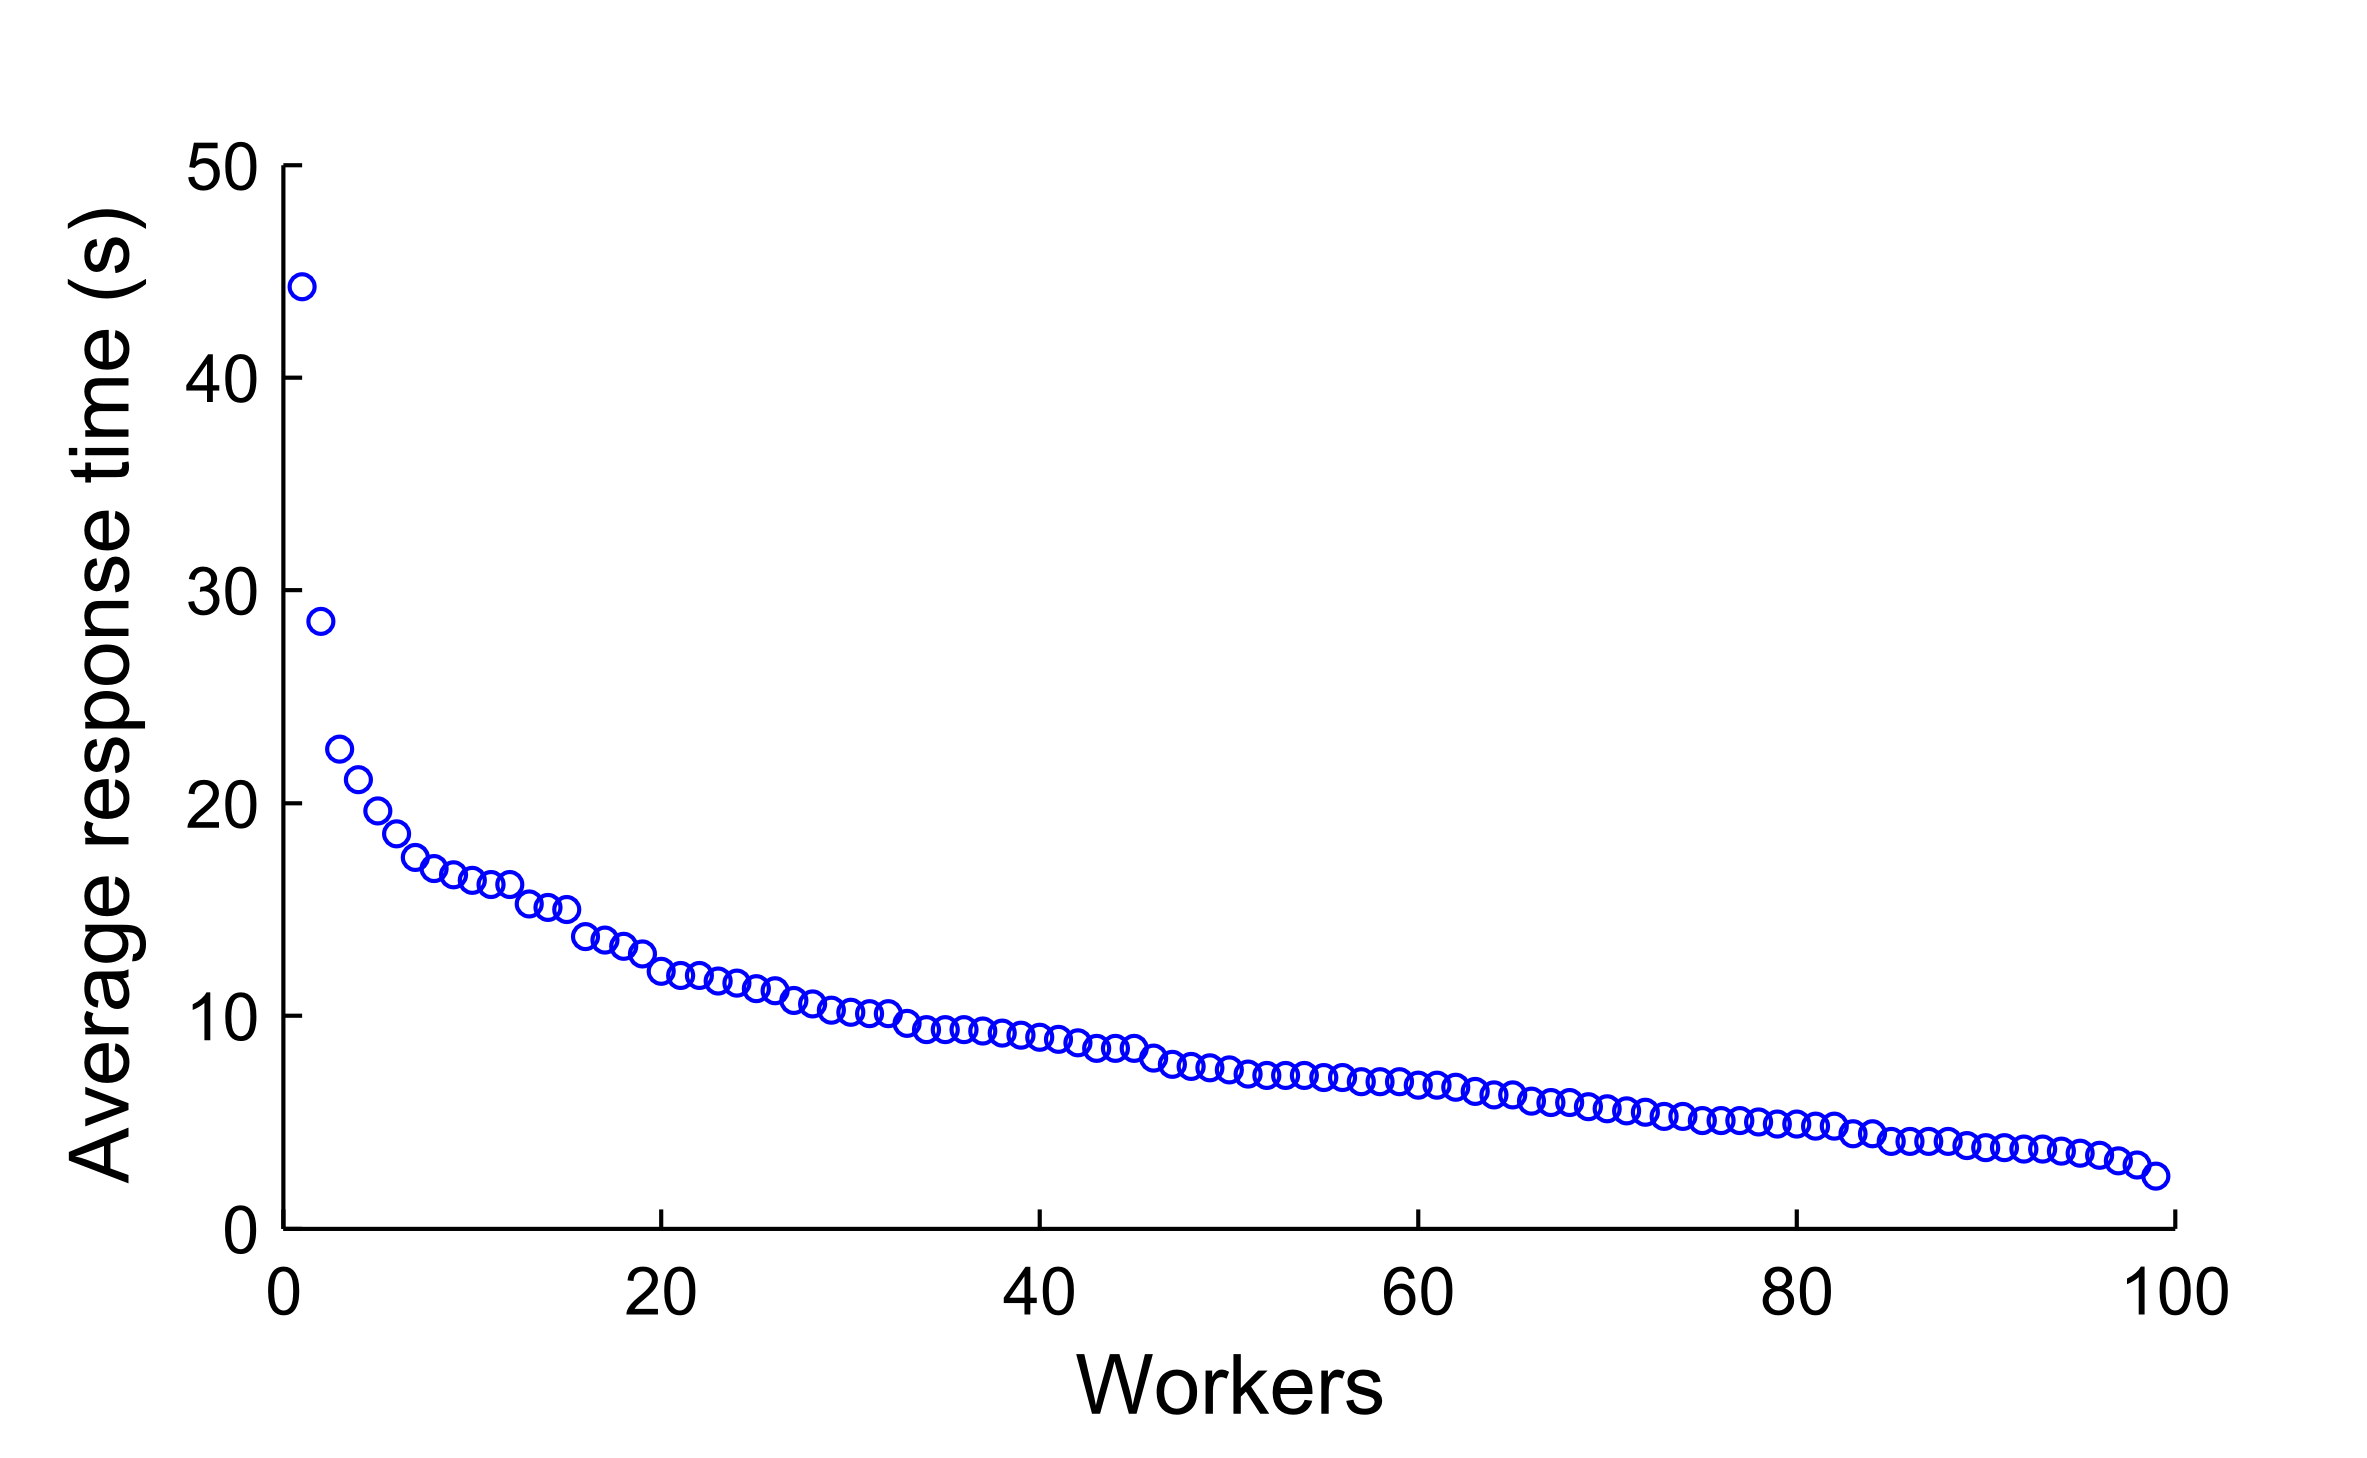
\includegraphics[width=10cm]{line_time_all_responses.png}
\caption{The ranked average response time for each worker.  }
\label{Figure: average_response_time}
\end{figure}



\section{Softmax model fitting}



\section{Initial Fusion Results}

%\begin{figure}
%	\centering
%		\begin{subfigure}{0.5\textwidth}
%			\centering
%			\setlength\figurewidth{10cm}
%    		\setlength\figureheight{5cm}  
%    		\inputTikZ{0.5}{responses_1-99_find0.5_train_on_all.fig.tikz}
%        	\subcaption{}\label{Subfigure:posterior responses raw 0.5}
%        \end{subfigure}%
%       	\begin{subfigure}{0.5\textwidth}
%			\centering
%			\setlength\figurewidth{10cm}
%    		\setlength\figureheight{5cm}  
%    		\inputTikZ{0.5}{responses_1-99_find0.7_train_on_all.fig.tikz}
%        	\subcaption{}\label{Subfigure:posterior responses raw 0.7}
%        \end{subfigure}%
%    	\\
%    	\begin{subfigure}{0.5\textwidth}
%			\centering
%			\setlength\figurewidth{10cm}
%    		\setlength\figureheight{5cm}  
%    		\inputTikZ{0.5}{responses_1-99_find0.4_train_on_all.fig.tikz}
%        	\subcaption{}\label{Subfigure:posterior responses raw 0.4}
%        \end{subfigure}%
%        \begin{subfigure}{0.5\textwidth}
%			\centering
%			\setlength\figurewidth{10cm}
%    		\setlength\figureheight{5cm}  
%    		\inputTikZ{0.5}{responses_1-99_find0.1_train_on_all.fig.tikz}
%        	\subcaption{}\label{Subfigure:posterior responses raw 0.1}
%        \end{subfigure}%
%        \caption{Examples of posterior estimate of circles position with increasing number of responses. Here the softmax model has been trained on all the available data}
%        \label{Figure: posterior responses raw}
%\end{figure}



FIGURE shows the typical impact on the posterior distribution as reports arrive, in the case of unfiltered data, with all of the dataset having been used to train the softmax model. 
In general the posterior becomes more peaked as more reports arrive. We can see in FIGURE that the distribution tends towards the true value as more reports arrive. 
In FIGURE we can see that as we increase the number of reports, the estimate becomes more stable. 
In FIGURE, we see an example of the reports leading to a poor estimate of circle position. 
In this case, there is a bias in the model that leads to the mean to be over estimated.  





The main process used for this analysis was to train the softmax model using approximately 50\% of the data, and then test the performance using the remaining data. 
This is repeated through several simulated runs, where the training data is randomly sampled from the full dataset. 


First, lets look at one typical simulation run. 
In this example, the circle is placed at the value 0.7. 
As we receive responses from workers, we can update our estimate of where the circle is. 
\ref{Figure:fusion_find_07} shows the impact of reports coming in on the mean and variance of the posterior distribution. 
Initially, we receive a report of 'NearTheLeft' which in this case leads to an inital poor estimate of the circles position. 
The next three reports all state 'NearTheRight' which has the effect of shifting the posterior mean towards the right and leading to an improved estimate of circle position. 
The complete posterior distribution is shown in \ref{Figure:fusion_find_07_dists}, which shows the reduction in variance as more reports arrive. 

\begin{figure}
	\centering
	\begin{subfigure}{6.5cm}
	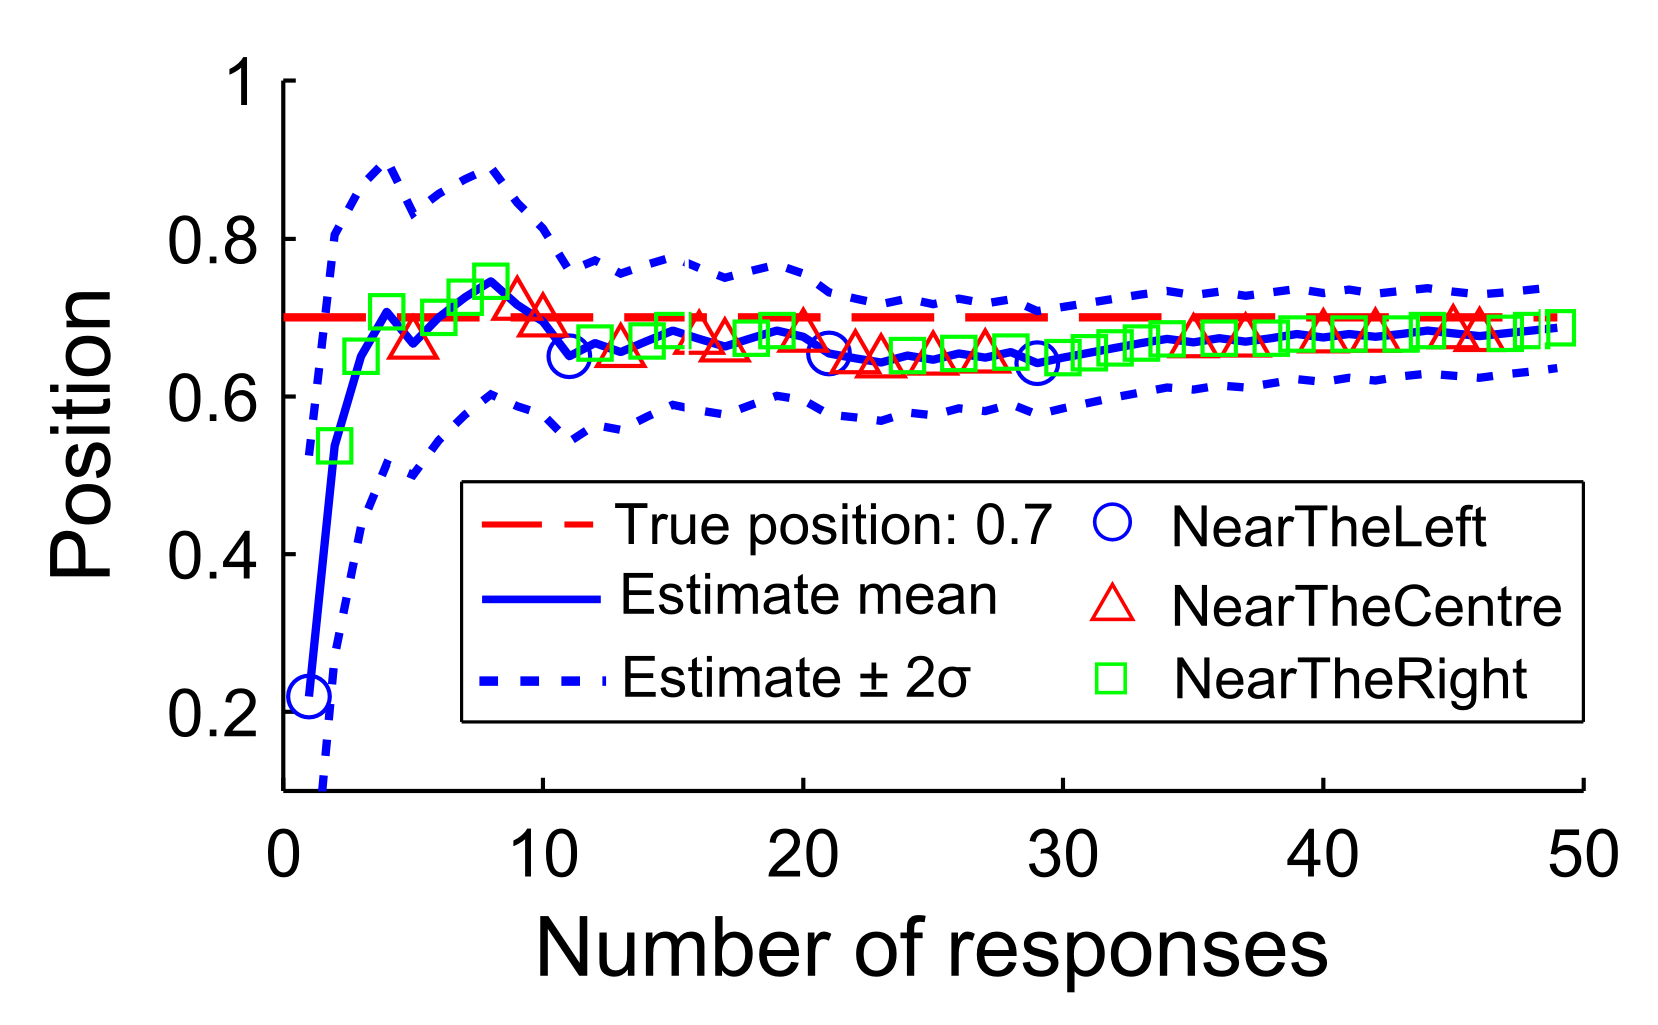
\includegraphics[width=6.5cm]{line_find_07.png}
	\caption{}
	\label{Figure:fusion_find_07}
	\end{subfigure}
	\begin{subfigure}{6.5cm}
	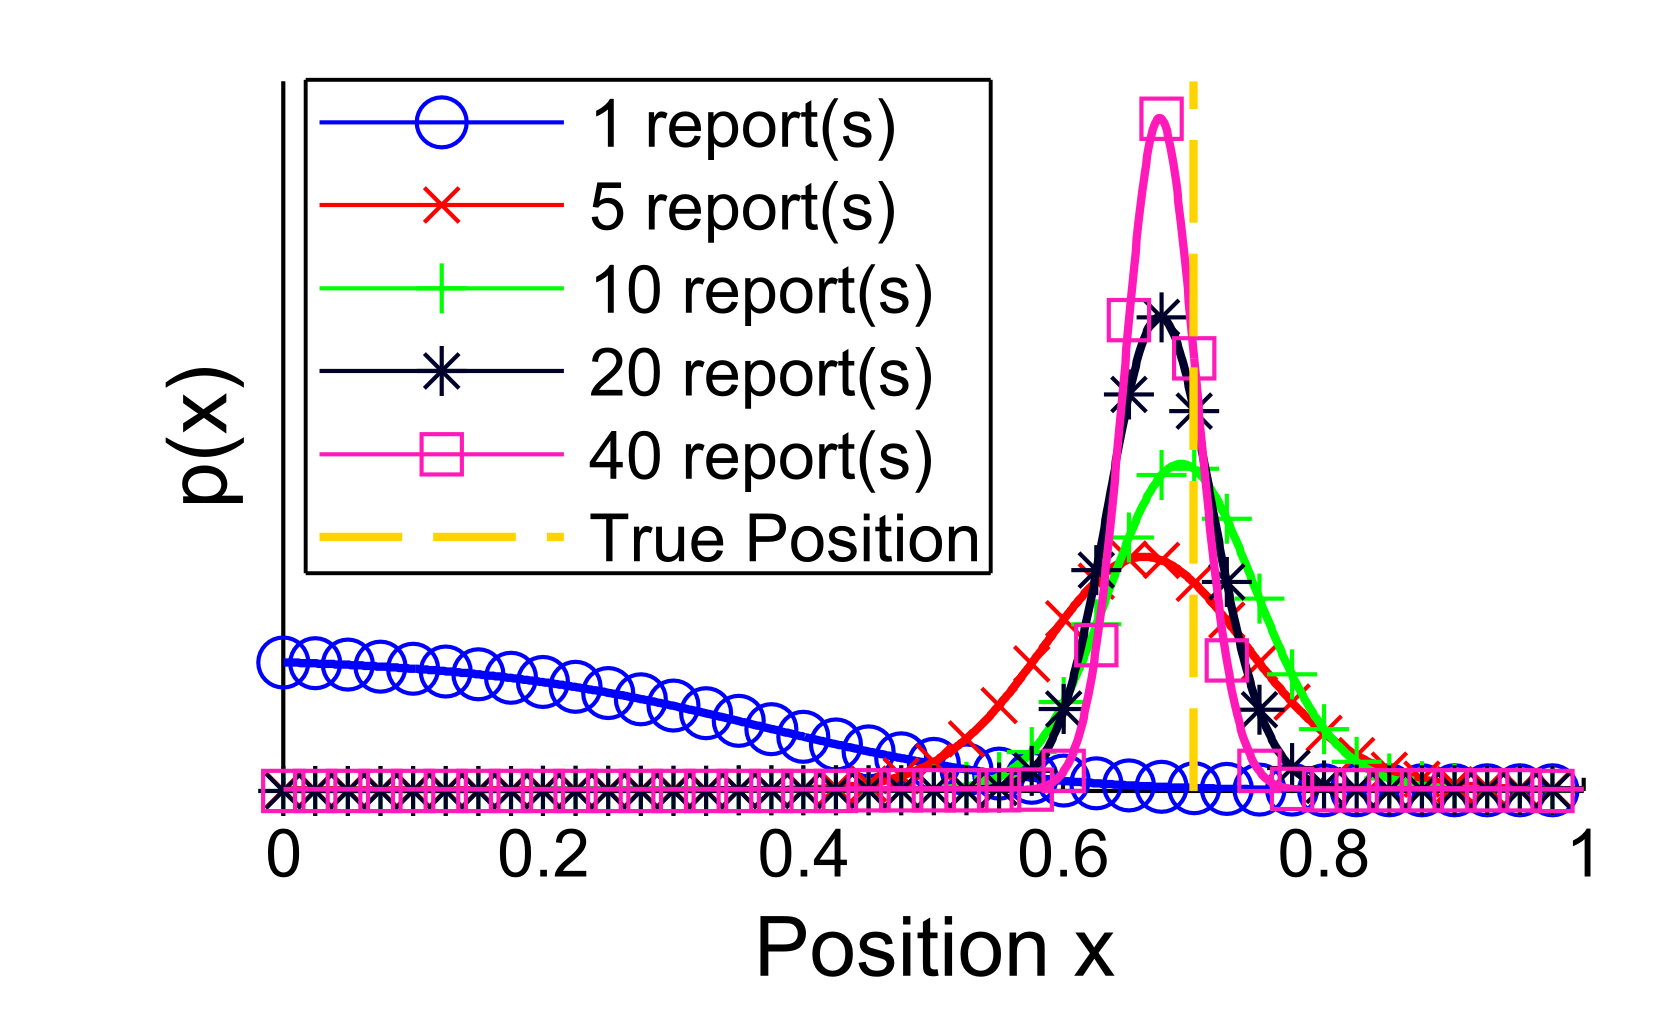
\includegraphics[width=6.5cm]{line_find_07_dists.png}
	\caption{}
	\label{Figure:fusion_find_07_dists}
	\end{subfigure}
	\caption{Estimating the position of the circle as new reports are received  \subref{Figure:fusion_find_07}) The change in posterior mean and variance with responses \subref{Figure:fusion_find_07_dists}) Examples of posterior distribution}
\end{figure}

\ref{Figure:MC RMSE} shows the RMSE for each circle position over 50 simulation runs, as the number of responses is increased. 
The RMSE was measured between the mean of the posterior distribution and the true circle position. 
The worst performance is achieved at the outer points 0.0 and 1.0. 
This can be attributed to the performance metric of the mean, or expectation value, of the distribution being used. 
At the outer regions of the experiment, the posterior distribution becomes heavily skewed, making the mean a poor summary statistic in this case. 
It is difficult to summarise multimodal or skewed distributions using a single metric.

The best performing position is 0.5. 
Again, this is to be expected as the mean of the 'NearTheCentre' likelihood function is close to 0.5, so if the majority of reports are of this type, we would expect a posterior with mean close to 0.5 even after only a small number of reports.


\begin{figure}
	\centering
	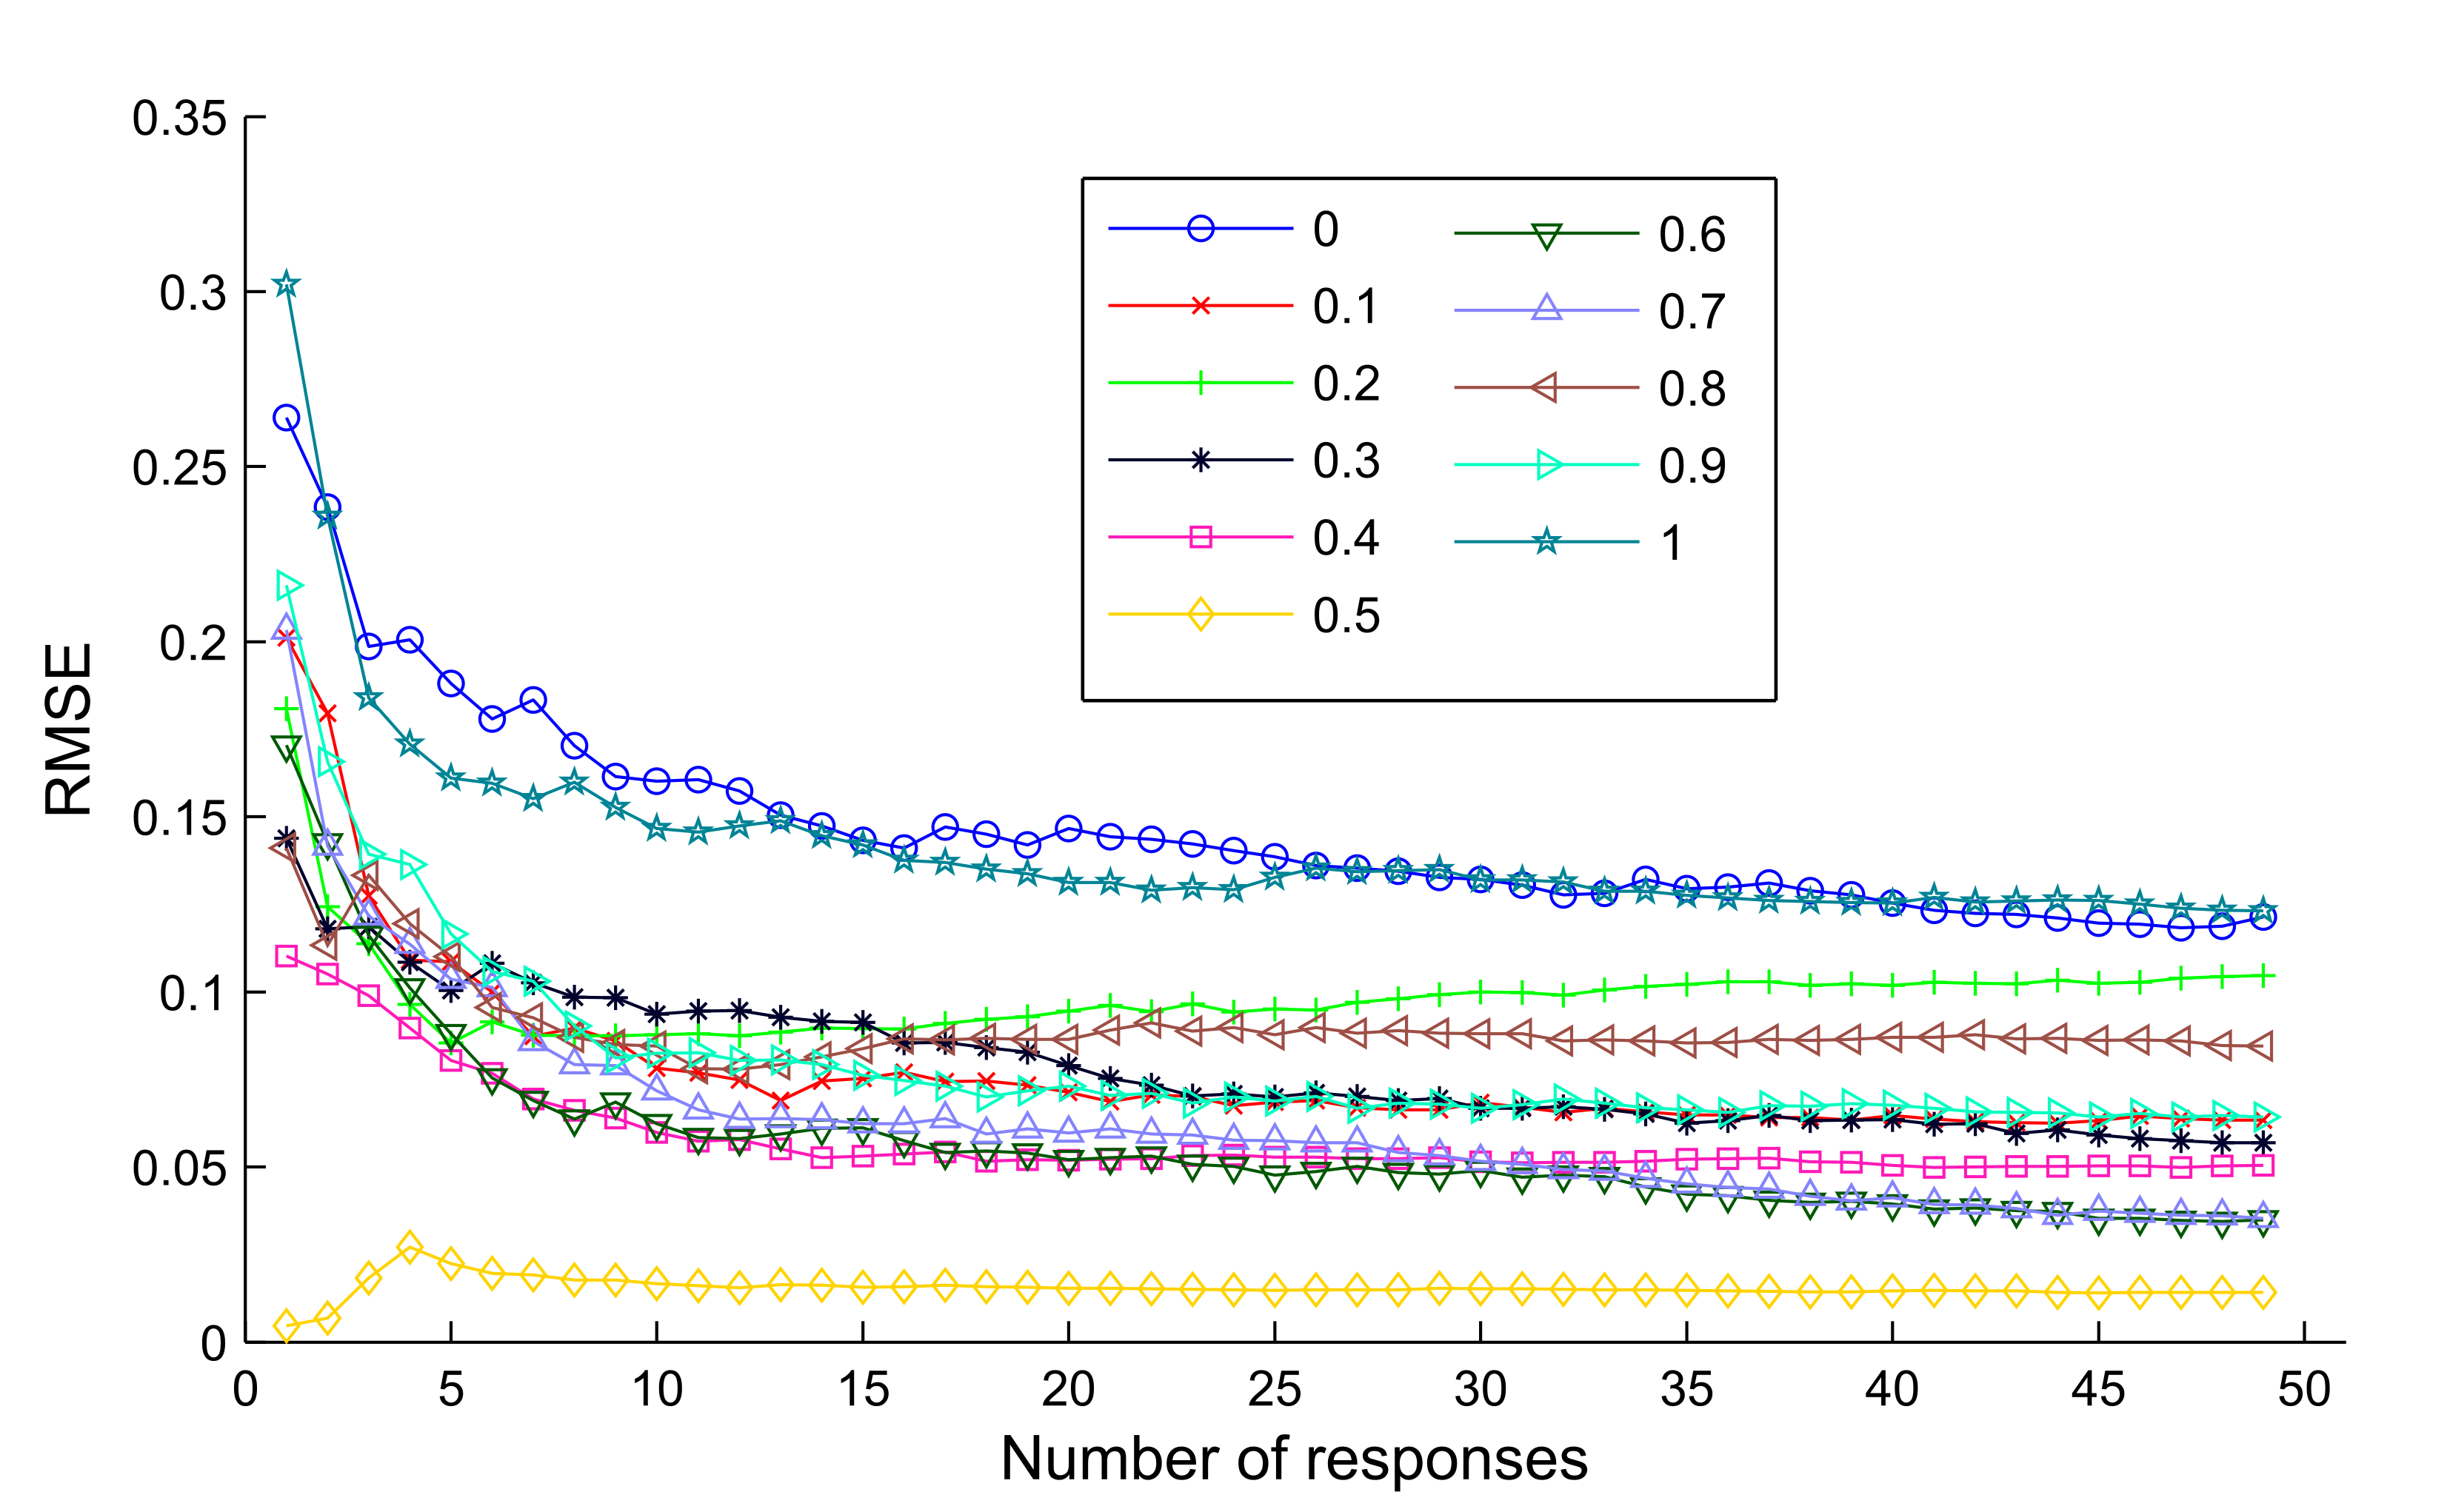
\includegraphics[scale=1]{line_RMSE.png}
	\label{Figure:MC RMSE}
	\caption{The Root-Mean-Square-Error of the posterior with the circle at varying positions, as the number of responses is increased. The RMSE was generated over 50 simulation runs}
\end{figure}


We can view the performance of the fusion by viewing the true circle position against the predicted circle position. 
This is shown in \ref{Figure: response_estimate}

\begin{figure}
\centering
\begin{subfigure}{6cm}
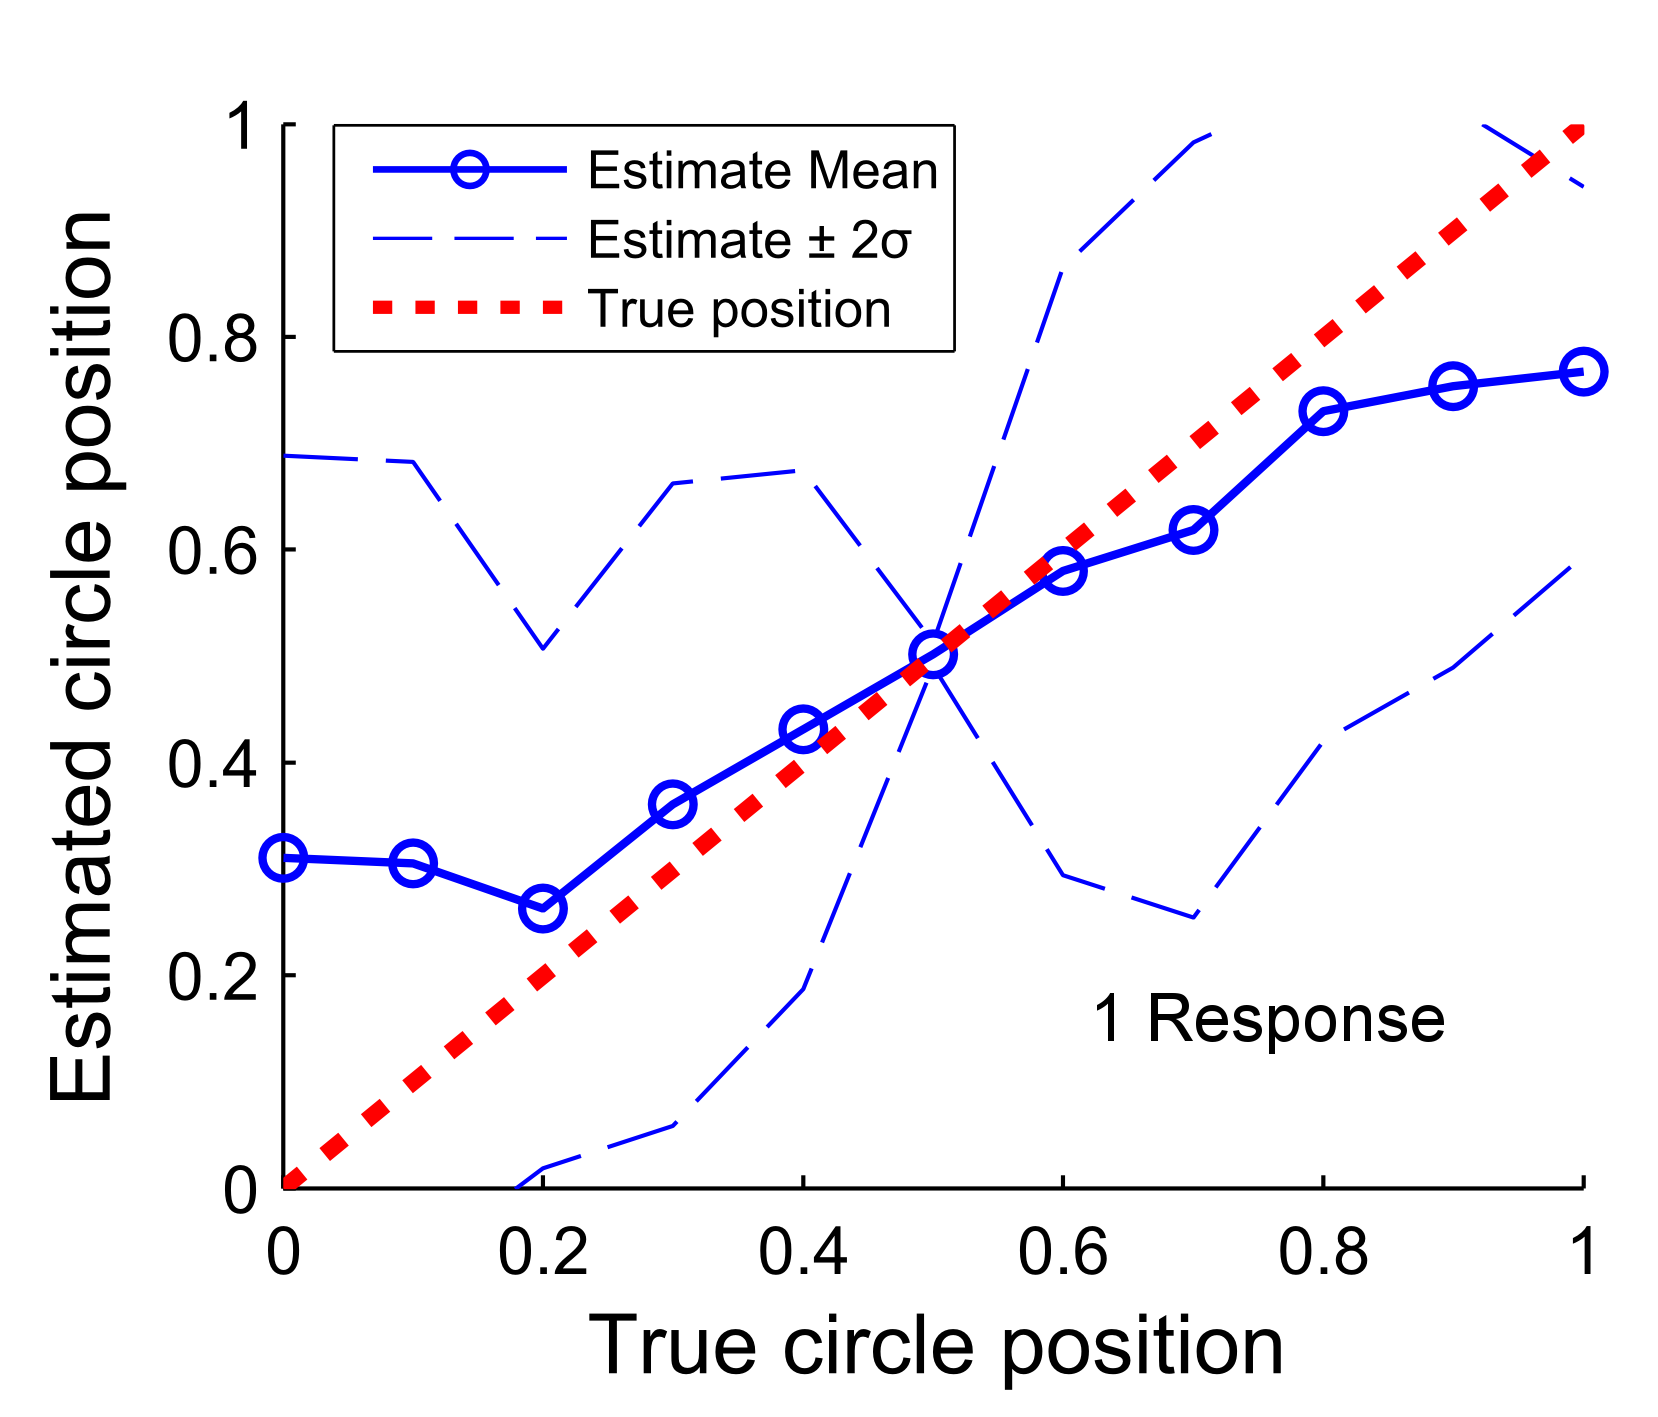
\includegraphics[width=6cm]{line_mc_1res_estimate.png}
\caption{}
\label{Figure: response_estimate_1}
\end{subfigure}
\begin{subfigure}{6cm}
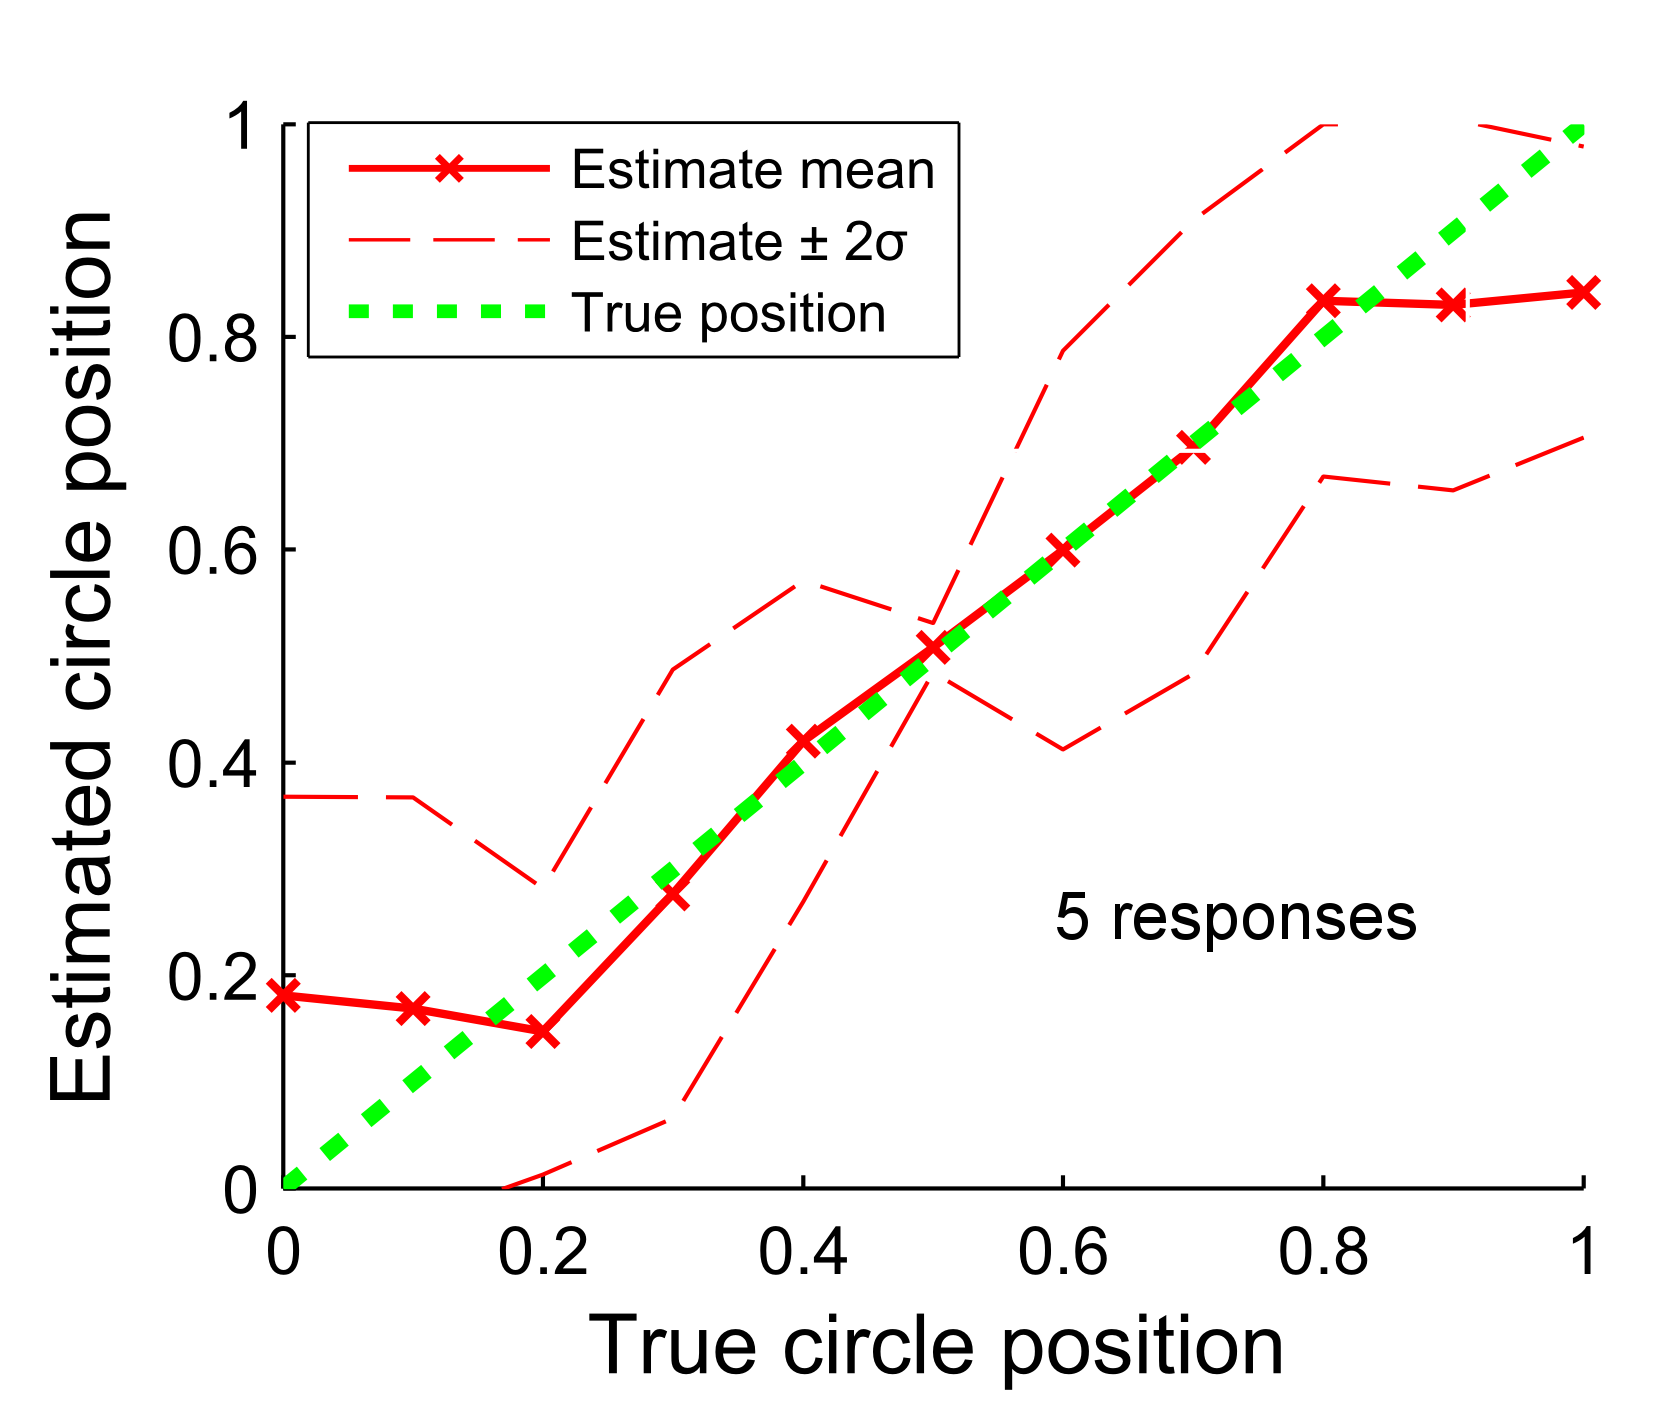
\includegraphics[width=6cm]{line_mc_5res_estimate.png}
\caption{}
\label{Figure: response_estimate_5}
\end{subfigure}\\
\begin{subfigure}{6cm}
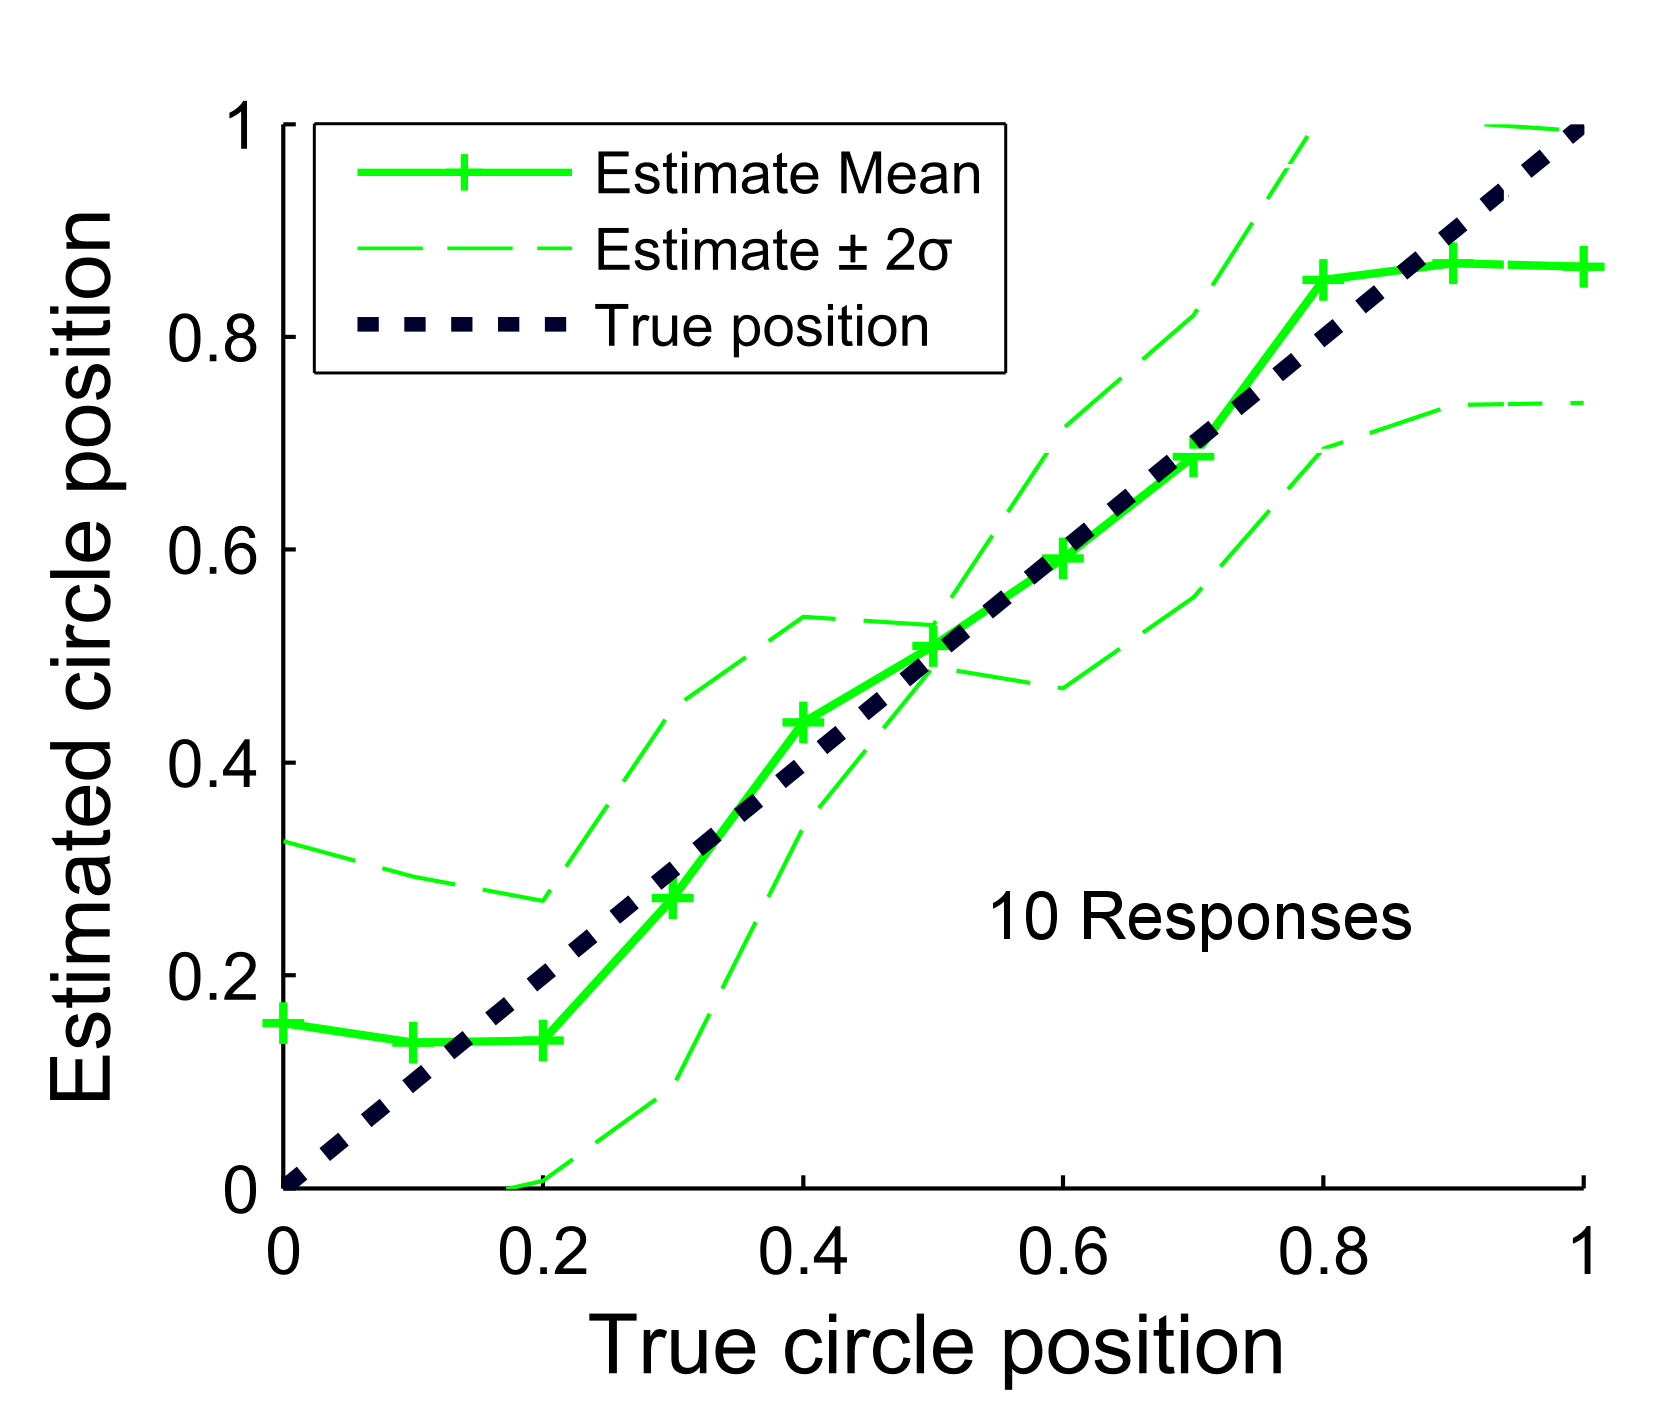
\includegraphics[width=6cm]{line_mc_10res_estimate.png}
\caption{}
\label{Figure: response_estimate_10}
\end{subfigure}
\begin{subfigure}{6cm}
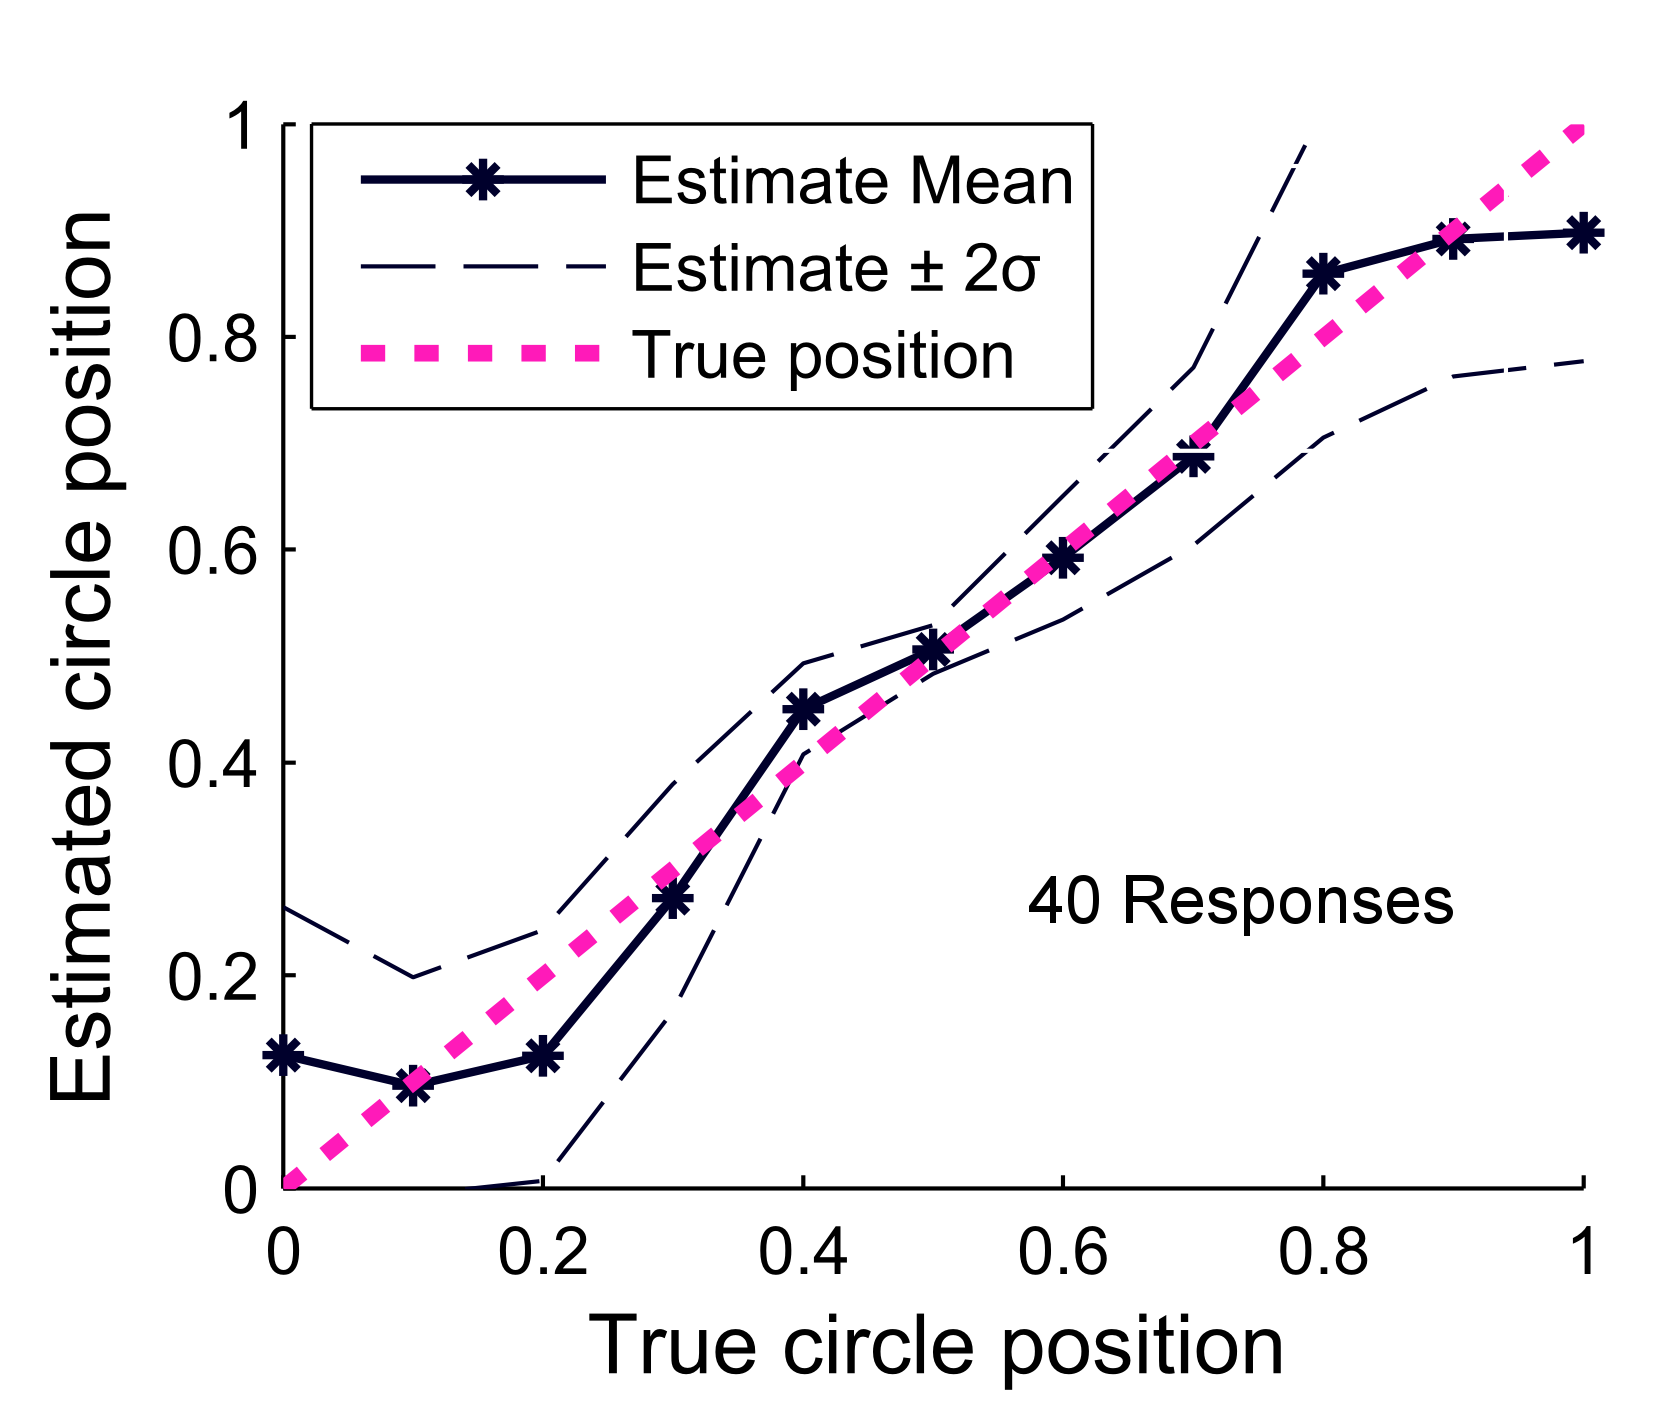
\includegraphics[width=6cm]{line_mc_40res_estimate.png}
\caption{}
\label{Figure: response_estimate_40}
\end{subfigure}
\caption{The mean performance of estimating the circle's position. The mean line is the average expectation value taken from 50 simulations runs. The standard deviations are for the deviations in the expectation values (not to be confused with the variance in the posterior distribution). The mean lines were generated using varying numbers of responses for each circle positon, with: \subref{Figure: response_estimate_1}) 1 response \subref{Figure: response_estimate_5}) 5 responses \subref{Figure: response_estimate_10})10 responses \subref{Figure: response_estimate_40}) 40 responses}
\label{Figure: response_estimate}
\end{figure}





\section{Limiting the worker variety/models}

It might seem intuitive to think that in an ideal world, for the purposes of data fusion, everyone would have the same response model i.e. the number of unique response models is one. 
That way we would know precisely the internal model that a person was using, and we could fit an accurate function to this. 
To test this intuition, a series of experiments were carried out in order to see the impact of limiting the variety of models found in the data. 

\subsection{Approach}

As shown in \ref{Figure:bar unique response model groups}, the number of unique models in the dataset with more than 1 worker associated to it was found to be 10. 
To investigate the impact of response model variety, these 10 models were used to create a series of training and testing datasets. 
10 datasets were created in total.

The first dataset contained only the responses from the workers with the most popular response model, the model shown in \ref{Figure:one worker model}. 
This dataset contained the responses from 16 workers in total. 
The second dataset contained only the responses from the first and second most popular response models, which totalled 21 workers. 
This process was continued, with the tenth dataset containing the top 10 response models.

These datasets were then used to train the softmax model. 
As the datasets were now different sizes, only 8 randomly selected workers (half the number of workers in the first dataset) from each dataset were used to train the model, and then 8 remaining workers were randomly selected used to test the model. This process was carried out for 100 experimental runs for each dataset. 

\subsection{Model fitting}










\subsection{State Estimation Results}

\ref{Figure: fusion top 10 popular models} shows the results of fusing different numbers of models. 
In \ref{Subfigure:fusion 1-5 popular models}, we can see that using 1 response model, then our mean estimate of circle position after fusion essentially follows the response model - the shape is qualitatively the same.  
As the number of models is increased, the mean estimate is improved. Increasing from 6-10 models shows little improvement in mean estimate. This is likely due to the small training and testing sets used.
 As response models 6-10 have relatively few workers in them compared to models 1-5, then the chances of them being sampled for training or testing purposes is relatively small.

%\begin{figure}
%	\centering
%		\begin{subfigure}{0.5\textwidth}
%			\centering
%			\setlength\figurewidth{10cm}
%    		\setlength\figureheight{10cm}  
%    		\inputTikZ{0.5}{line_models1-5_means.tikz}
%        	\subcaption{}\label{Subfigure:fusion 1-5 popular models}
%        \end{subfigure}%
%        \begin{subfigure}{0.5\textwidth}
%			\centering
%			\setlength\figurewidth{10cm}
%    		\setlength\figureheight{10cm}  
%    		\inputTikZ{0.5}{line_models6-10_means.tikz}
%    		\subcaption{}\label{Subfigure:fusion 6-10 popular models}
%        \end{subfigure}%
%        \caption{The mean estimate of circle position achieved by using 8 training workers and 8 testing workers over 100 simulation runs, sampled from datasets containing: \subref{Subfigure:fusion 1-5 popular models}) Top 5 popular response models; \subref{Subfigure:fusion 6-10 popular models}) Top 10 popular response models}
%        \label{Figure: fusion top 10 popular models}
%\end{figure}

In order to investigate the impact of the less popular response models, the same process was carried out using models 3-10. So for each dataset, the first two models were included. 
This increased the size of the dataset from 16, to 42 workers. The results are shown in \ref{Figure: fusion top 3-10 popular models}. 
These results show the same trend as the smaller dataset, with the increase in worker response models improving the data fusion results. 
The conclusion that can be drawn from this is that an increase in the variety of response models improves the overall fusion. 
We do not want all workers to behave the same, as is the case with 1 response model in \ref{Subfigure:fusion 1-5 popular models}. 
We want some spread of results, that gives each position of the circle as unique a input signature as possible. 
However, too much variety, and we would have an input that approximates noise.

%\begin{figure}
%	\centering
%		\begin{subfigure}{0.5\textwidth}
%			\centering
%			\setlength\figurewidth{10cm}
%    		\setlength\figureheight{10cm}  
%    		\inputTikZ{0.5}{line_models3-6_means.tikz}
%        	\subcaption{}\label{Subfigure:fusion 3-6 popular models}
%        \end{subfigure}%
%        \begin{subfigure}{0.5\textwidth}
%			\centering
%			\setlength\figurewidth{10cm}
%    		\setlength\figureheight{10cm}  
%    		\inputTikZ{0.5}{line_models7-10_means.tikz}
%    		\subcaption{}\label{Subfigure:fusion 7-10 popular models}
%        \end{subfigure}%
%        \caption{The mean estimate of circle position achieved by using 21 training workers and 21 testing workers over 100 simulation runs, sampled from datasets containing: \subref{Subfigure:fusion 3-6 popular models}) Top 6 popular response models; \subref{Subfigure:fusion 7-10 popular models}) Top 10 popular response models}
%        \label{Figure: fusion top 3-10 popular models}
%\end{figure}




%Figure, RMSE error for each number of models, with varaince in rmse over runs



%Variance should increase as the variety of dataset increases? 









\section{Data Filtering}

This section looks at the impact on the whole dataset using different data filtering approaches. 

\subsection{Common Models}

%FIGURE showing top 3, top 5, top 10



\subsection{Consistent Models}
%Figure showing all consistent,decreasing/increasing, and increasing only

\subsection{Symmetric Models}
%Figure showing all symmetric, and response symmetric


\subsubsection{}

\subsection{Gold Data Filtering}

\begin{figure}[!htb]
  \centering
  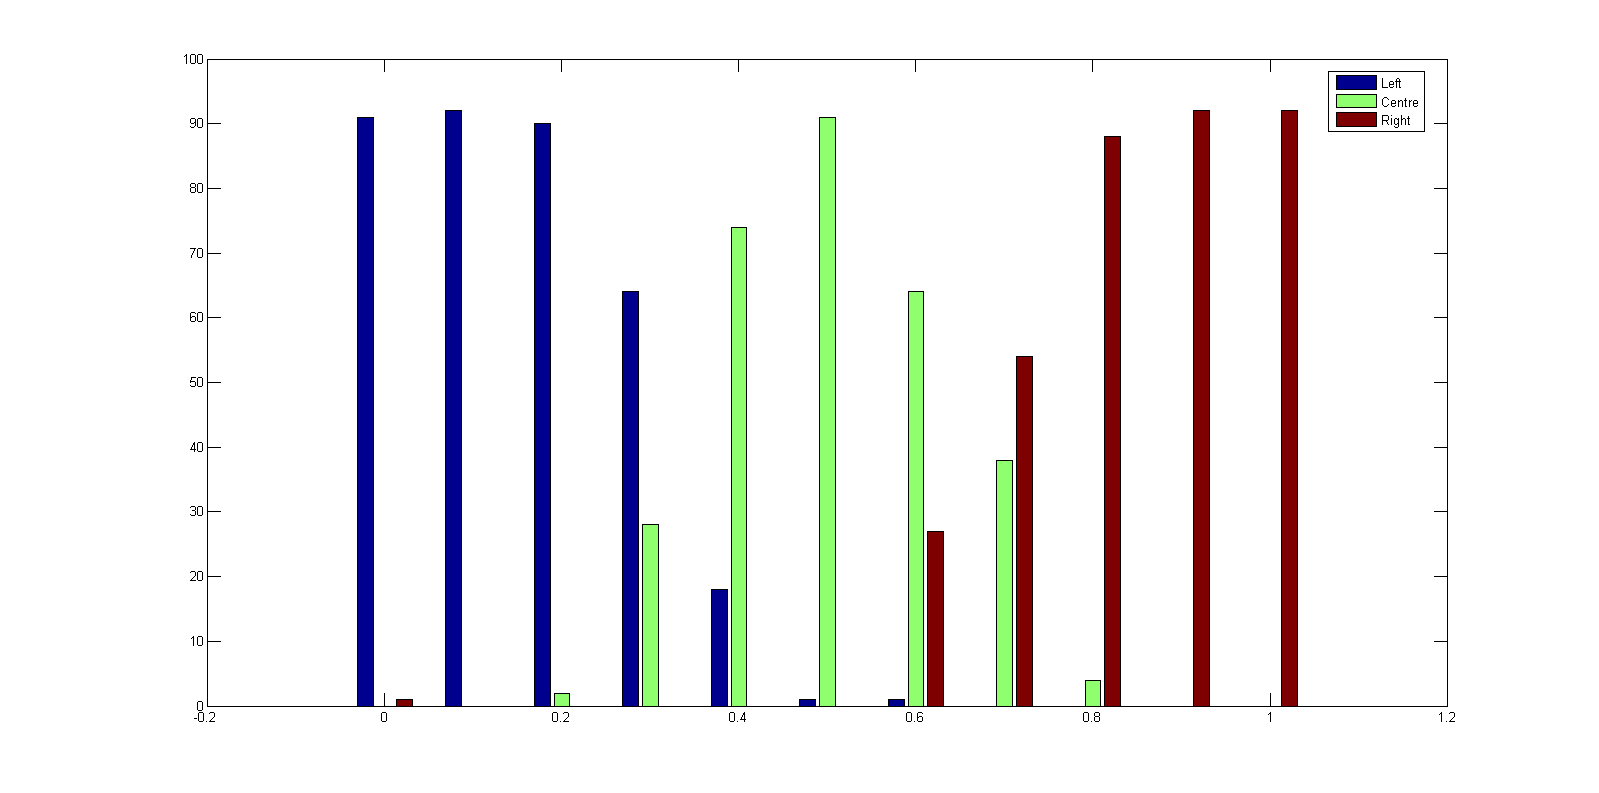
\includegraphics[width=8cm]{bar_responses_2_gold.png}
  \caption{The number of Left(Blue),Centre(Green) and Right(Red) worker responses at ground truth circle position after filtering the data using gold data and a threshold of 2 wrong answers}
  \label{Figure:bar responses 2 gold}
\end{figure}


%\begin{figure}[!htb]
%  \centering
%  \includegraphics[width=8cm]{bar_responses_1_gold.png}
%  \caption{The number of Left(Blue),Centre(Green) and Right(Red) worker responses at ground truth circle position after filtering the data using gold data and a threshold of 1 wrong answers}
%  \label{Figure:bar responses 1 gold}
%\end{figure}

Gold data filtering is a heuristic approach for filtering out poor performing workers.
 It relies on the creation of 'gold questions' ; questions where there is a known acceptable answer. 
 In this experiment, there is ambiguity about where the classes NearToLeft, NearToCentre, and NearToRight start and finish.
  However, we would expect all responders to answer NearToLeft when the circle was located at 0, and NearToRight when the circle is located at 1. 
  We can use these locations as gold questions, setting an expected response for each. 
  If a worker gets a threshold value (or greater) of gold questions wrong, then we not only ignore their responses for the gold question, but also all other questions as they are deemed to be unreliable or of poor quality. 

Using the ground truth locations of 0 and 1 as gold questions, the data was filtered. 
Setting the threshold at 2 (workers who got both gold questions wrong were ignored), the filtered responses are shown in \ref{Figure:bar responses 2 gold}. 

The result of setting the gold data threshold to 1 is shown in \ref{Figure:bar responses 1 gold}.


\subsection{Filtering comparisons}

%Table: Table showing the number of each report with each type of filtering, and the number of workers filtered out.
%\chapter{Circular Experiment}

Workers were asked where the circle was compared to a point in the image.
The circle was placed in 32 positions, with the angle between the dot and circle being varied. Each worker was asked to provide 16 responses.

Originally the workers were asked to provide all 32 responses, but no workers decided to  do this. 
It is unclear if this was due to the number of questions being asked, which was relatively high for each worker, or if it was another issue such as the time of posting the task. 




%Raw dataset
\begin{figure}
	\centering
	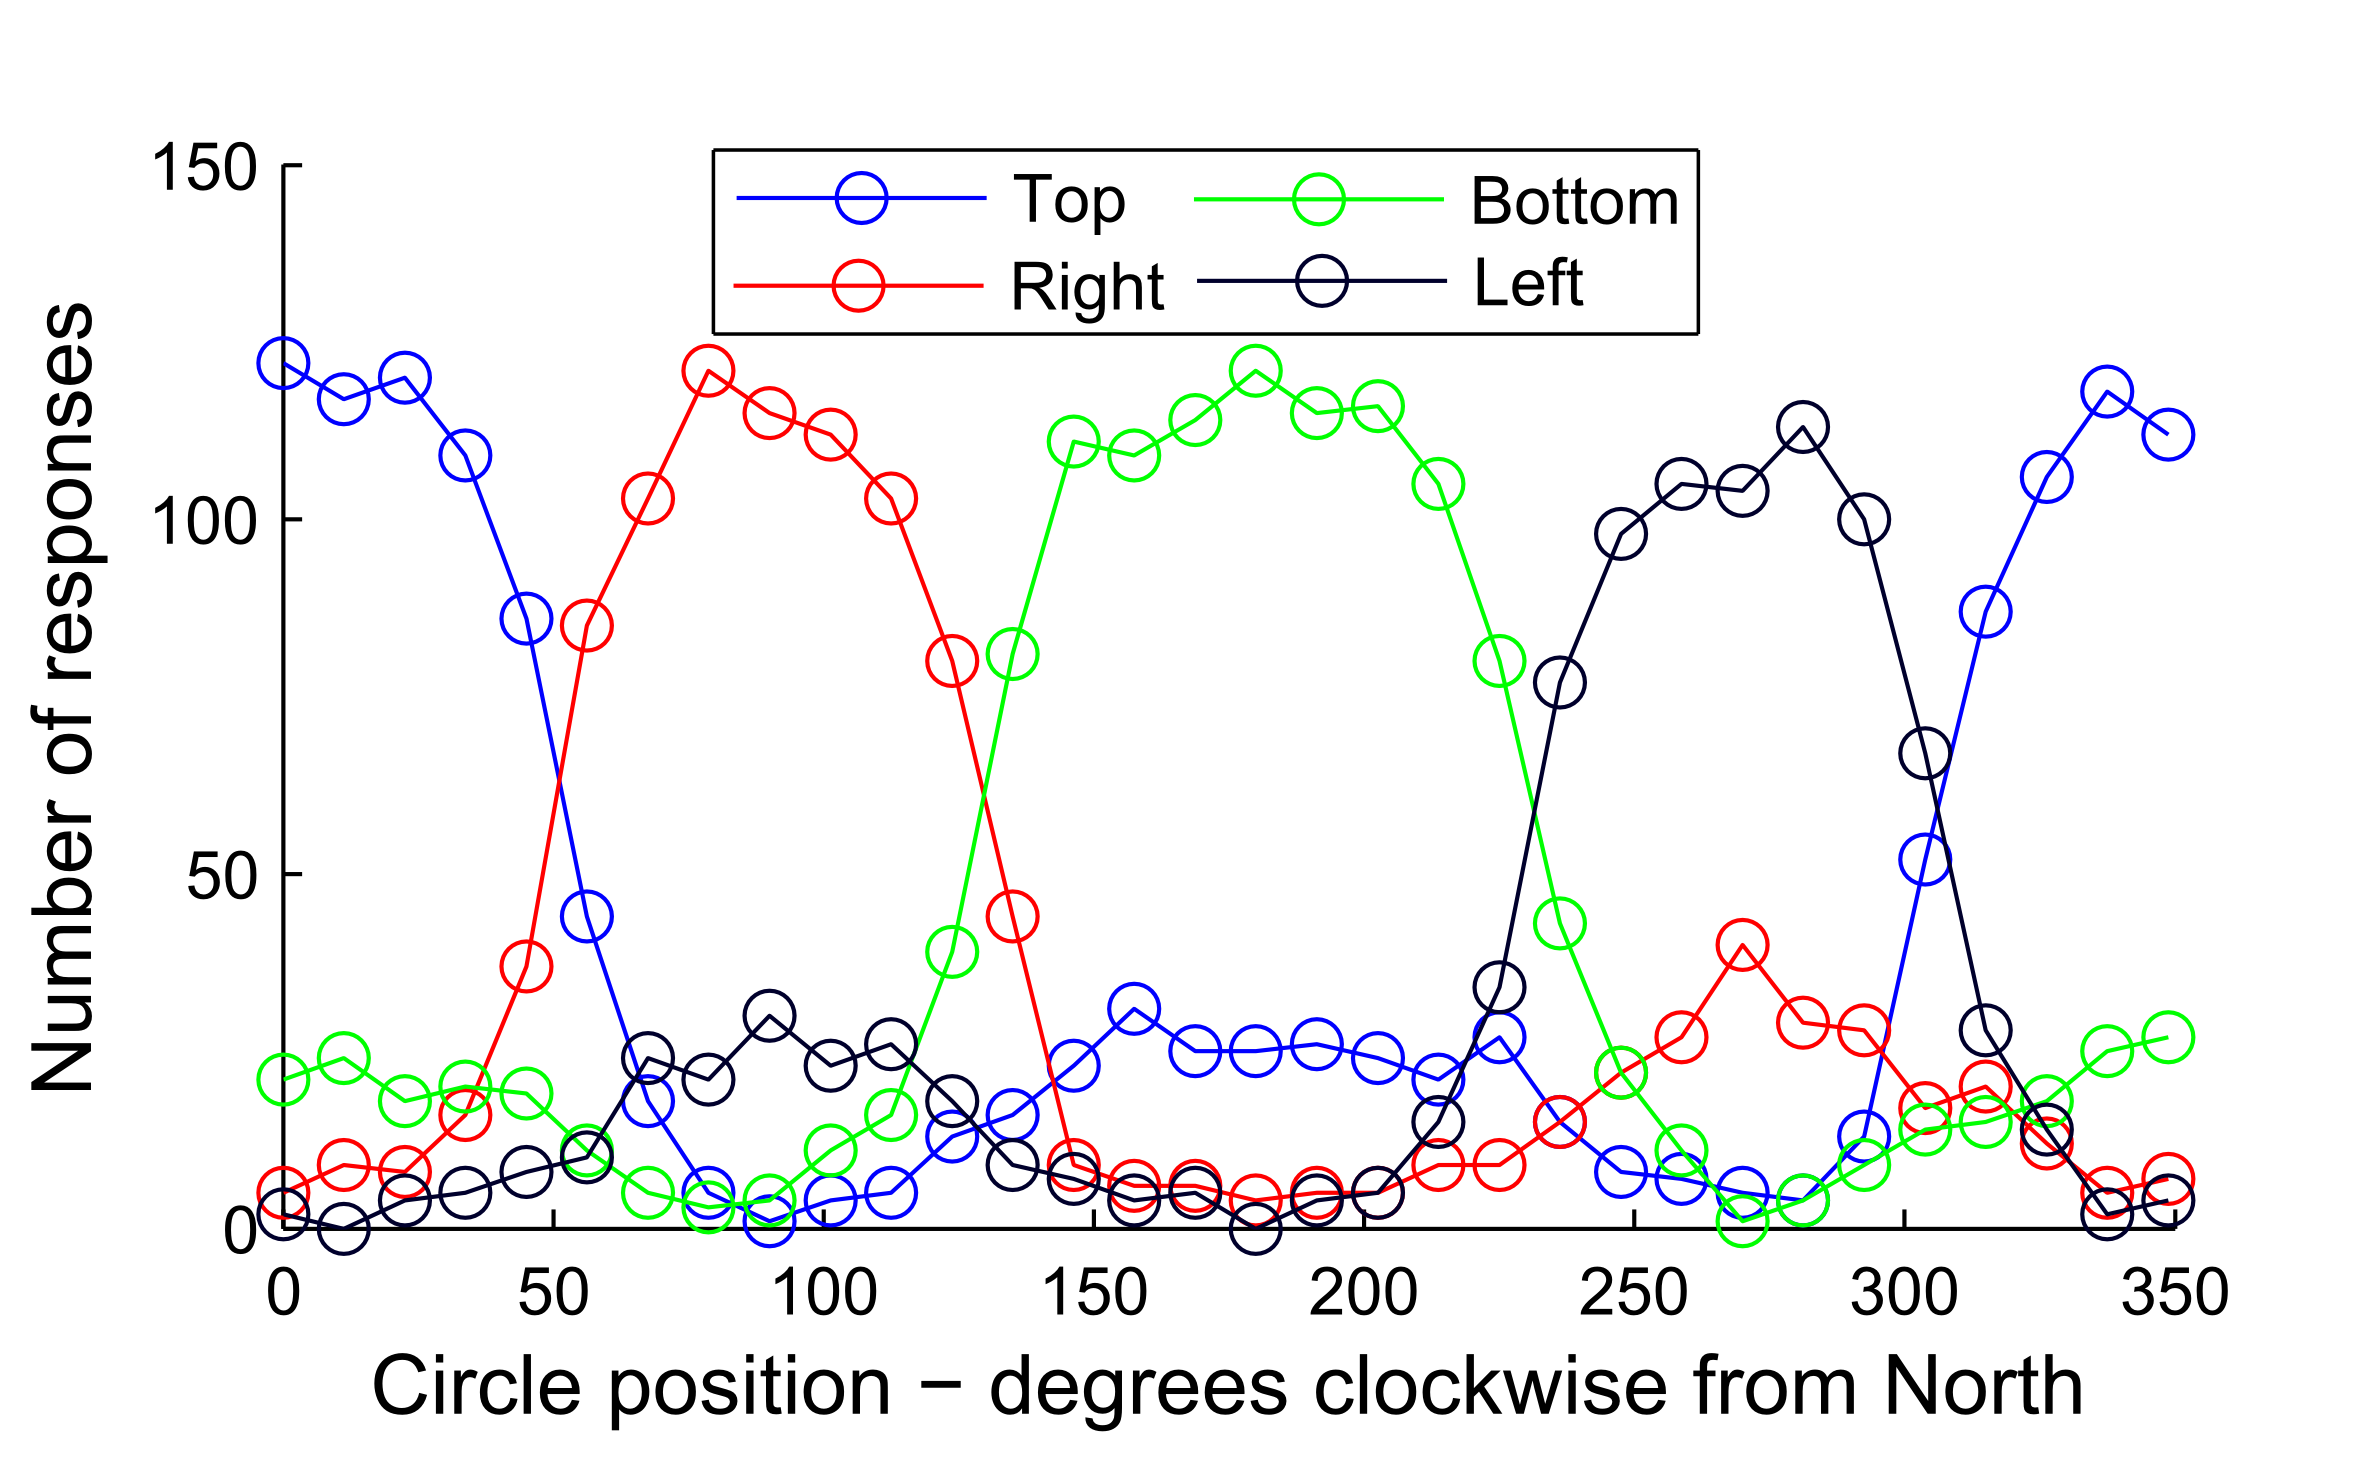
\includegraphics[scale=1]{line_circular_raw_data.png}
	\caption{The number of responses at each of the 32 circle positions}
	\label{Figure:circular_raw_responses}
\end{figure}

\begin{figure}
	\centering
	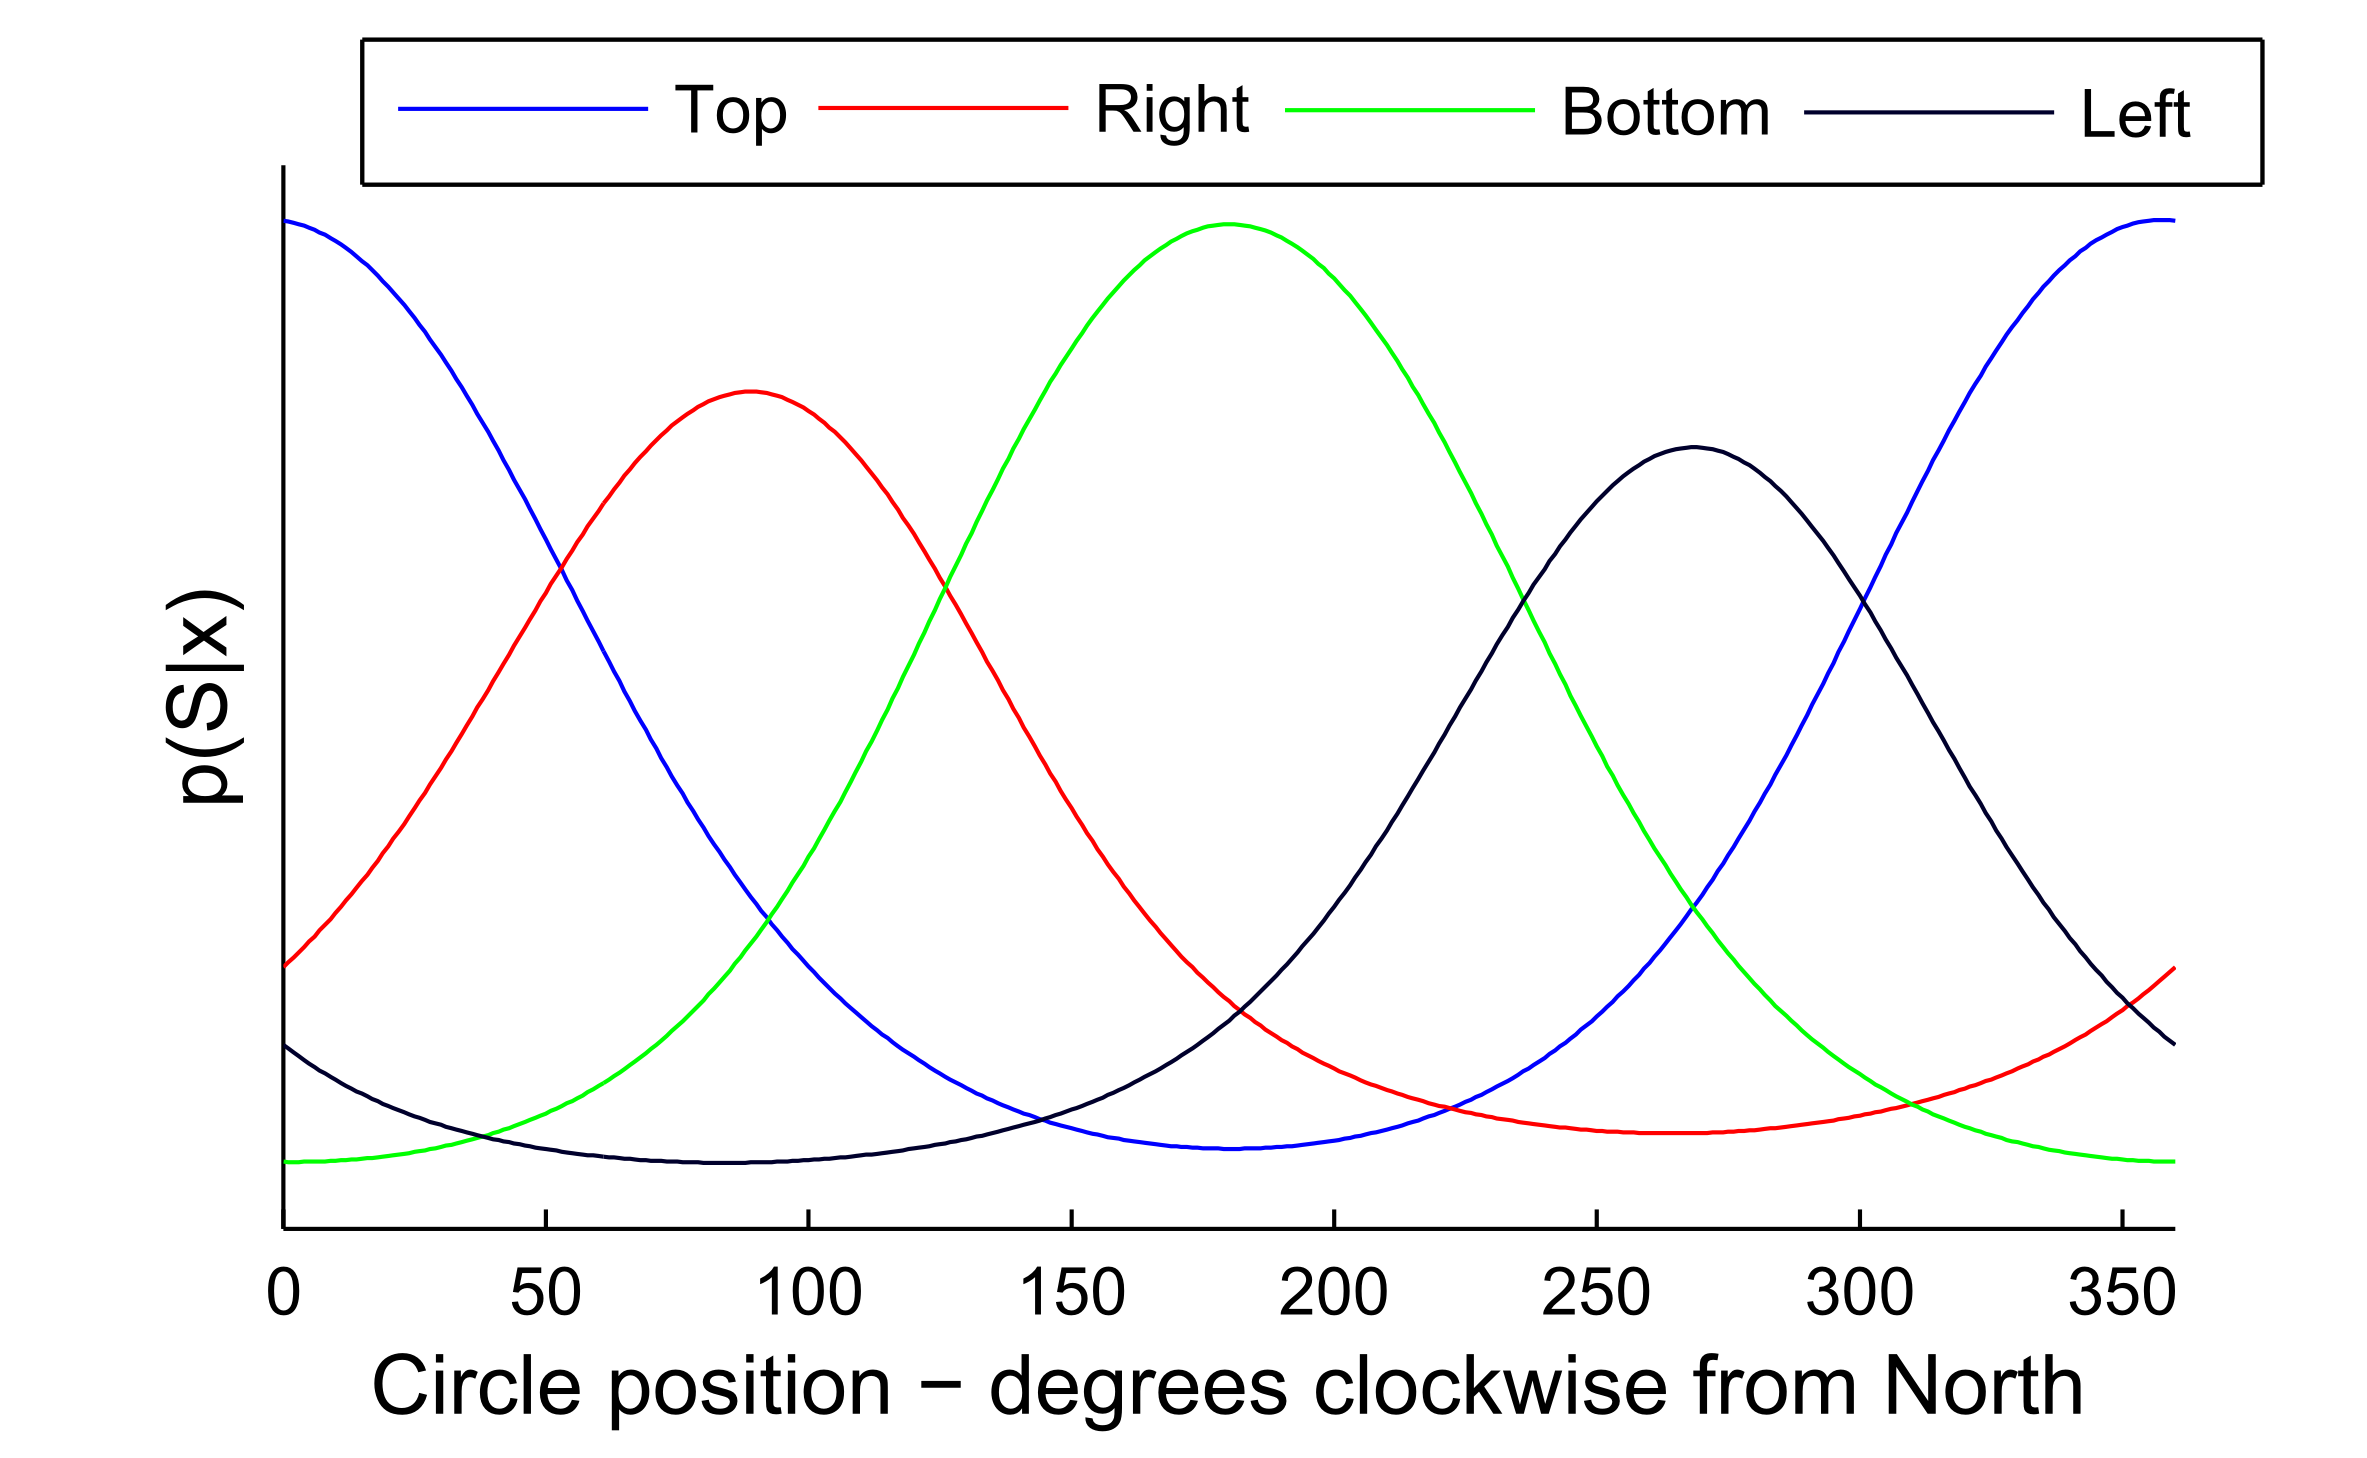
\includegraphics[scale=1]{line_circular_raw_data_softmax.png}
	\caption{The maximum likelihood softmax model for the raw data}
	\label{Figure:cicular_raw_softmax_model_all_responses}
\end{figure}




\begin{figure}
	\centering
	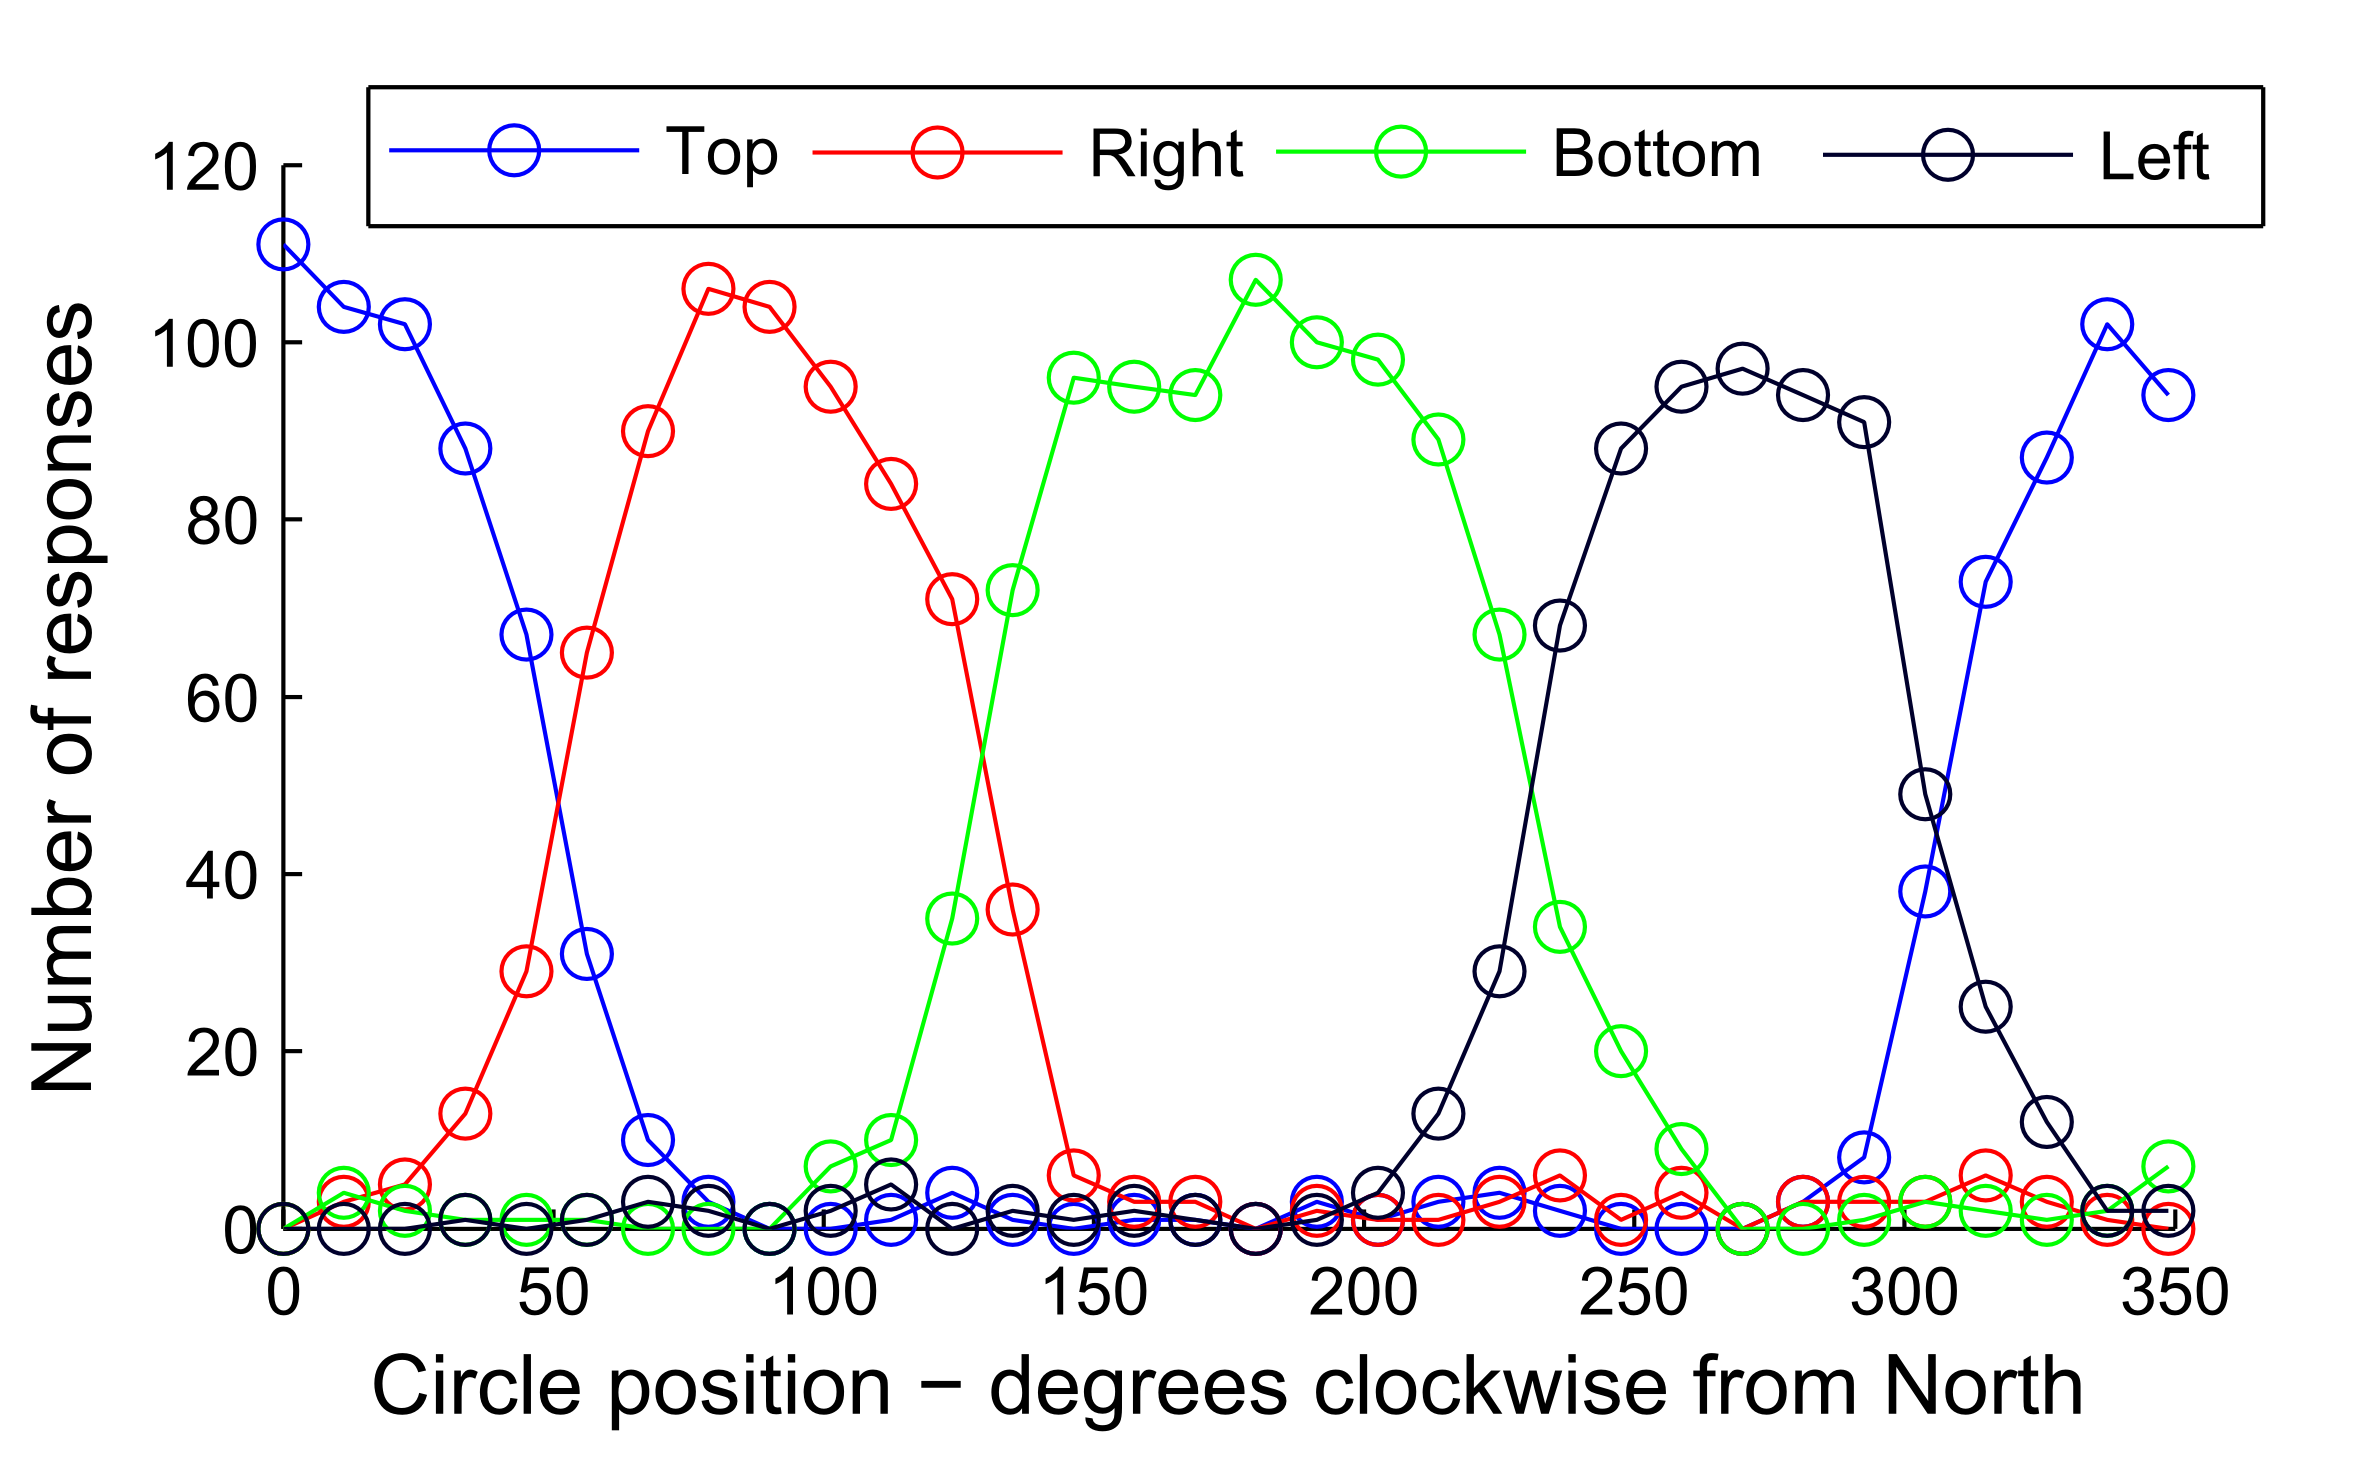
\includegraphics[scale=1]{line_circular_gold_responses.png}
	\caption{The gold data filtered responses. Gold responses were set at 0, 90, 180 and 270. If a worker got a single gold response incorrect, they were filtered out.}
	\label{Figure:cicular_gold_responses}
\end{figure}


\begin{figure}
	\centering
	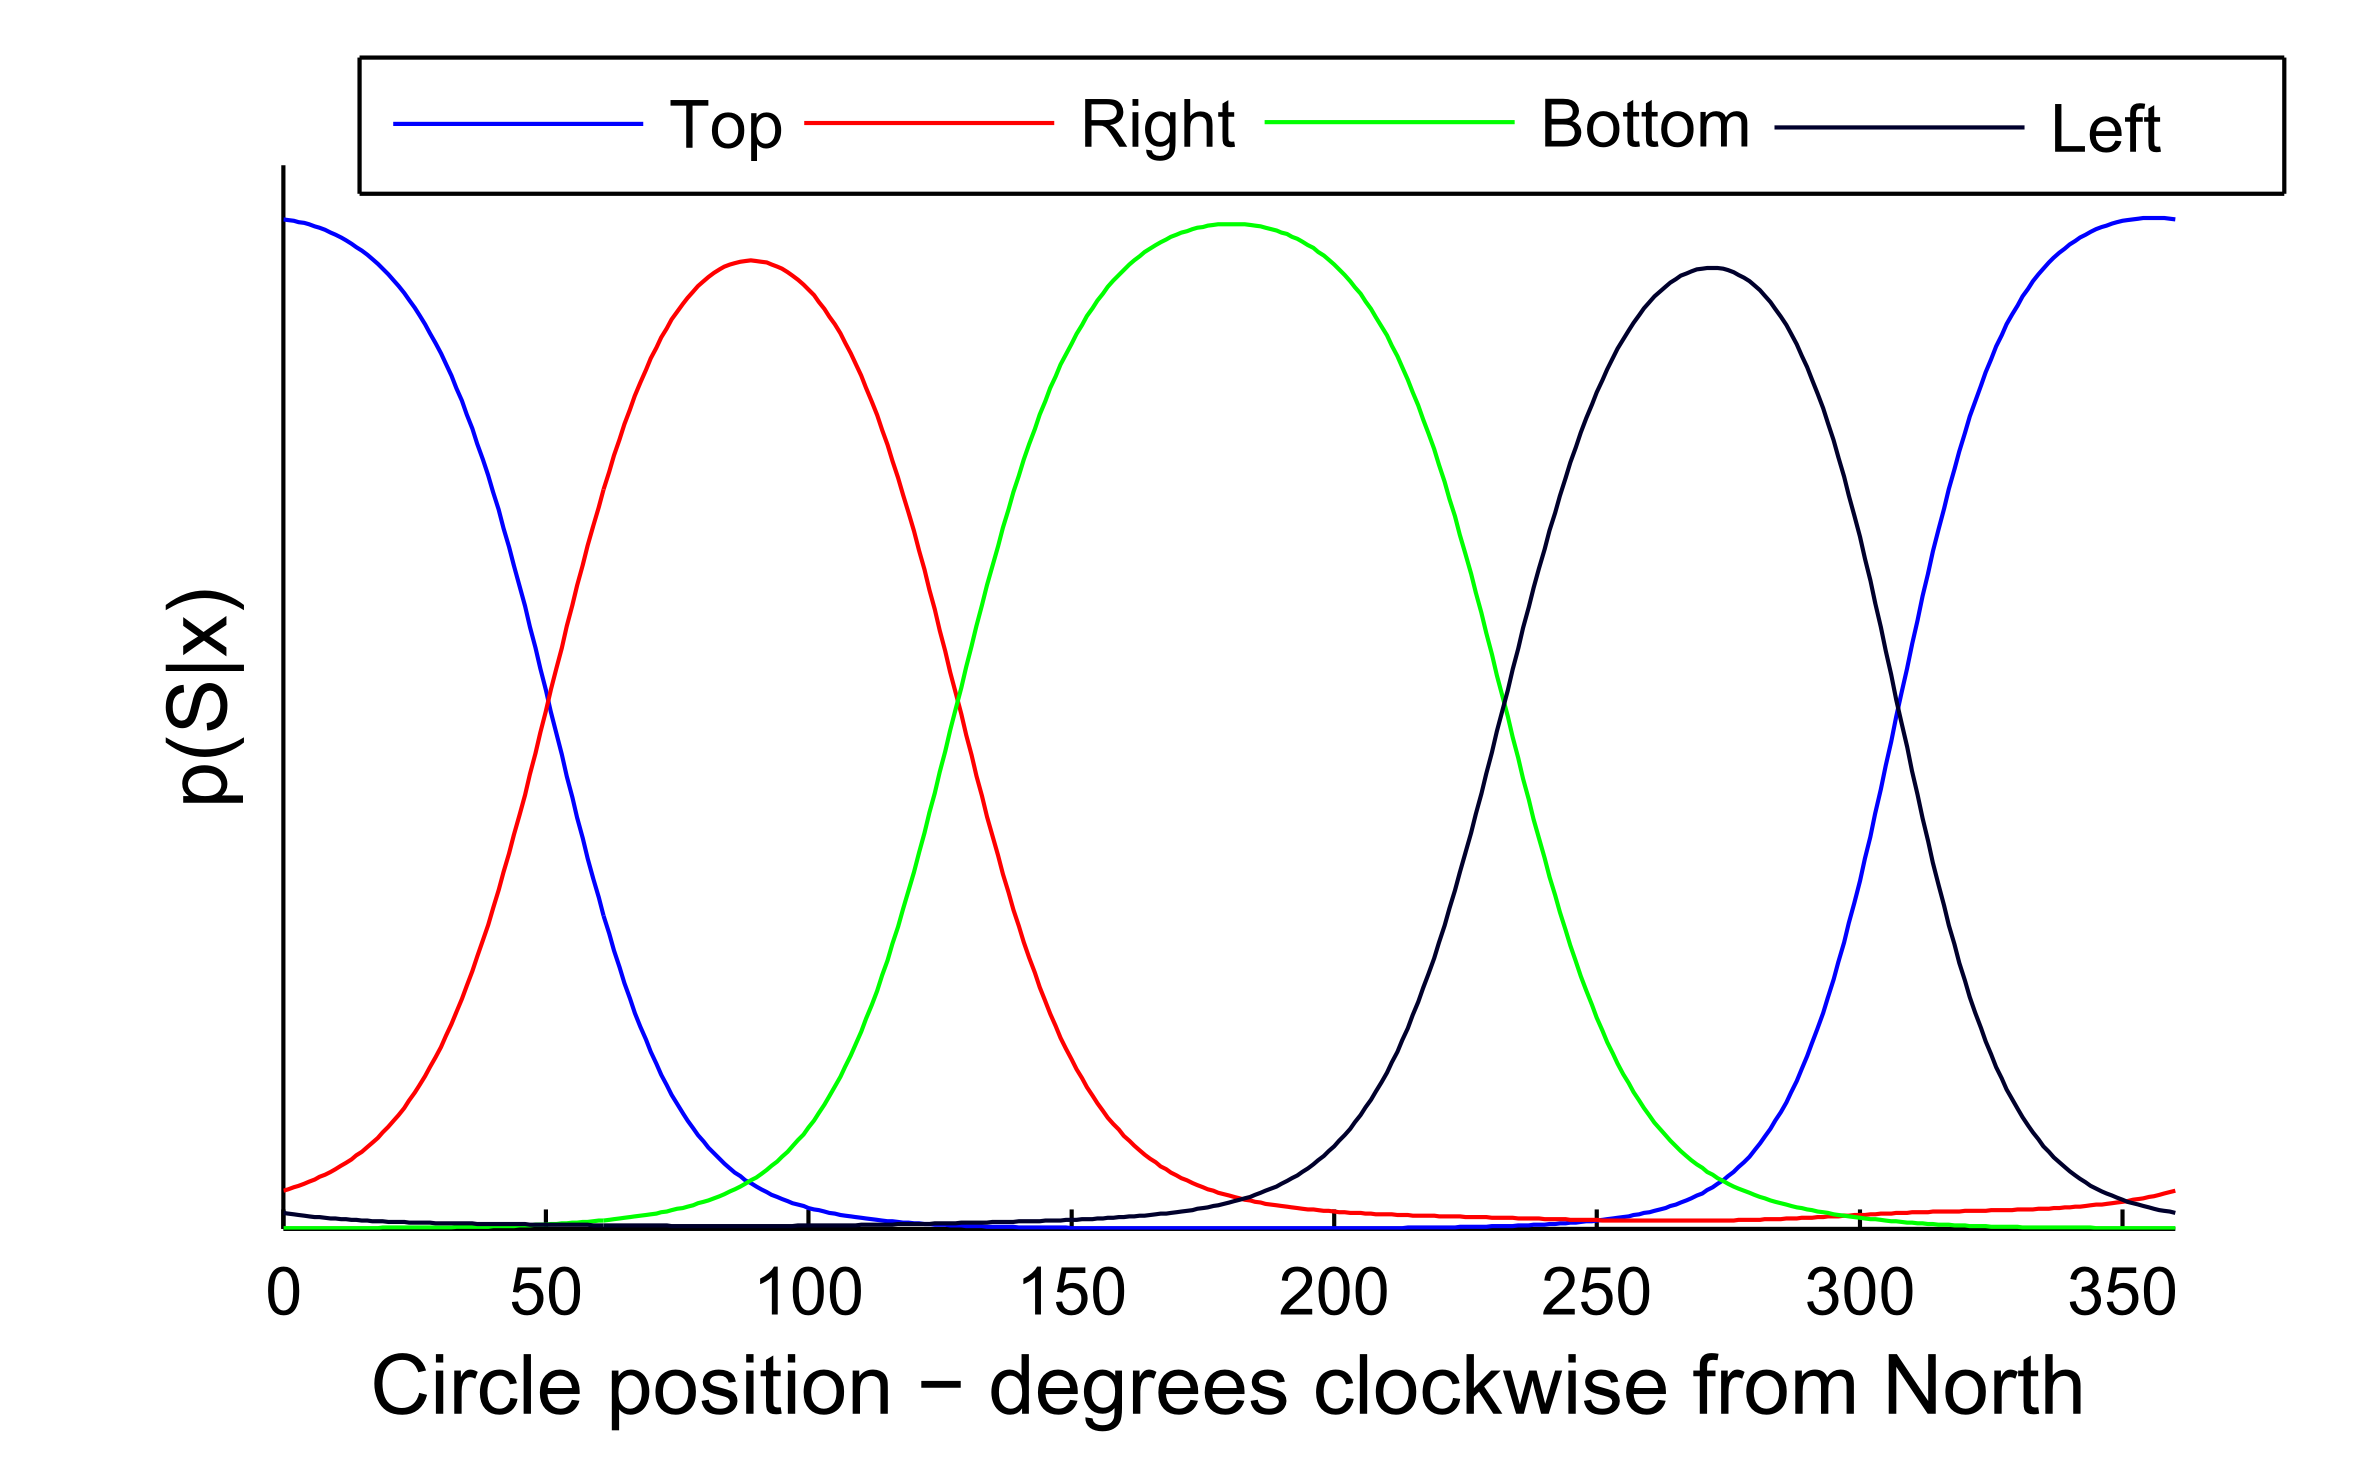
\includegraphics[scale=1]{line_circular_gold_softmax.png}
	\caption{The maximum likelihood softmax model for the gold filtered data.}
	\label{Figure:cicular_gold_softmax_model}
\end{figure}



\section{Data fusion}
\begin{figure}
	\centering
	\begin{subfigure}{7cm}
	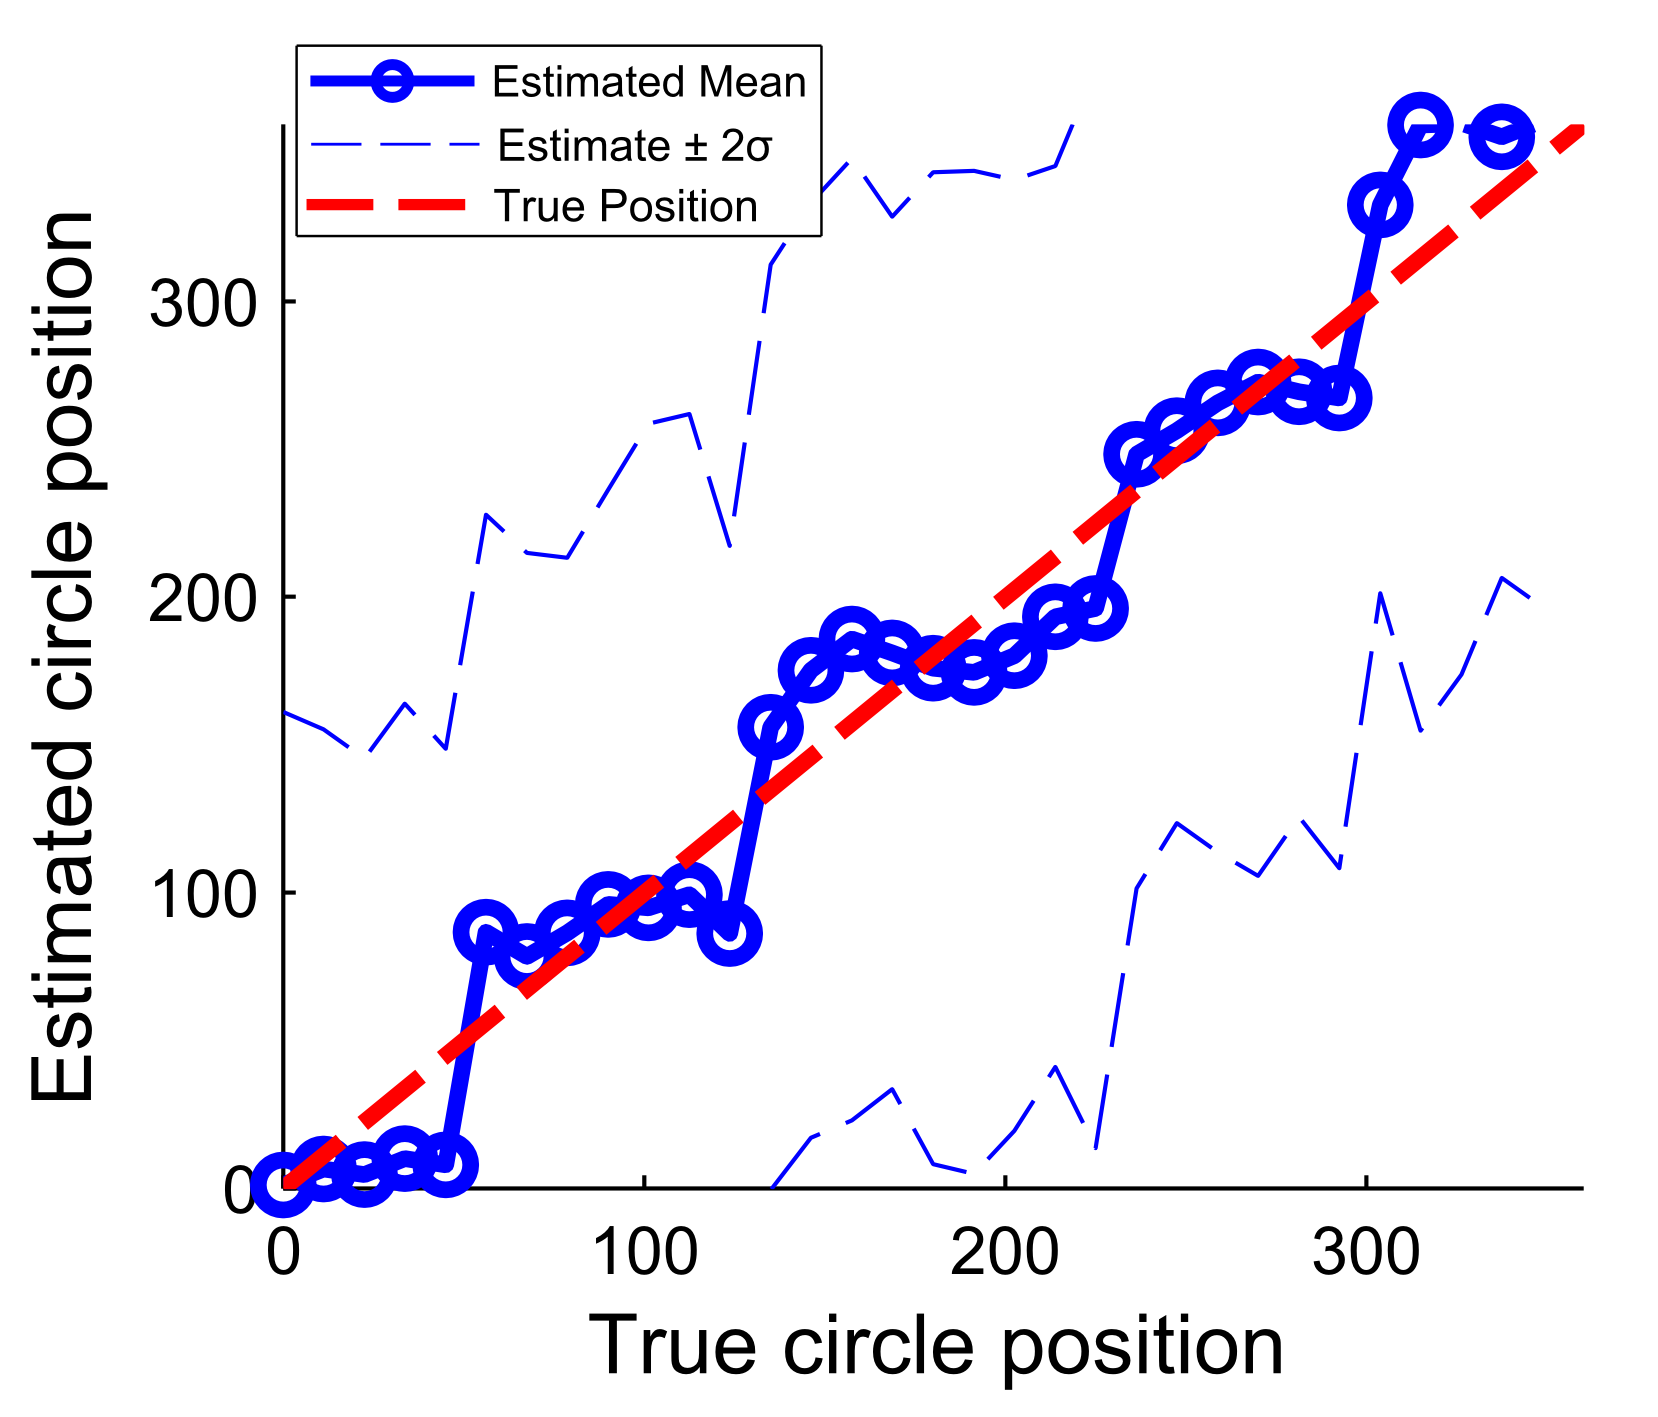
\includegraphics[scale=1]{circular_line_fusion_mean_1report.png}
	\caption{}	
	\label{Figure: circular_fusion_mean_1}
	\end{subfigure}
	\begin{subfigure}{7cm}
	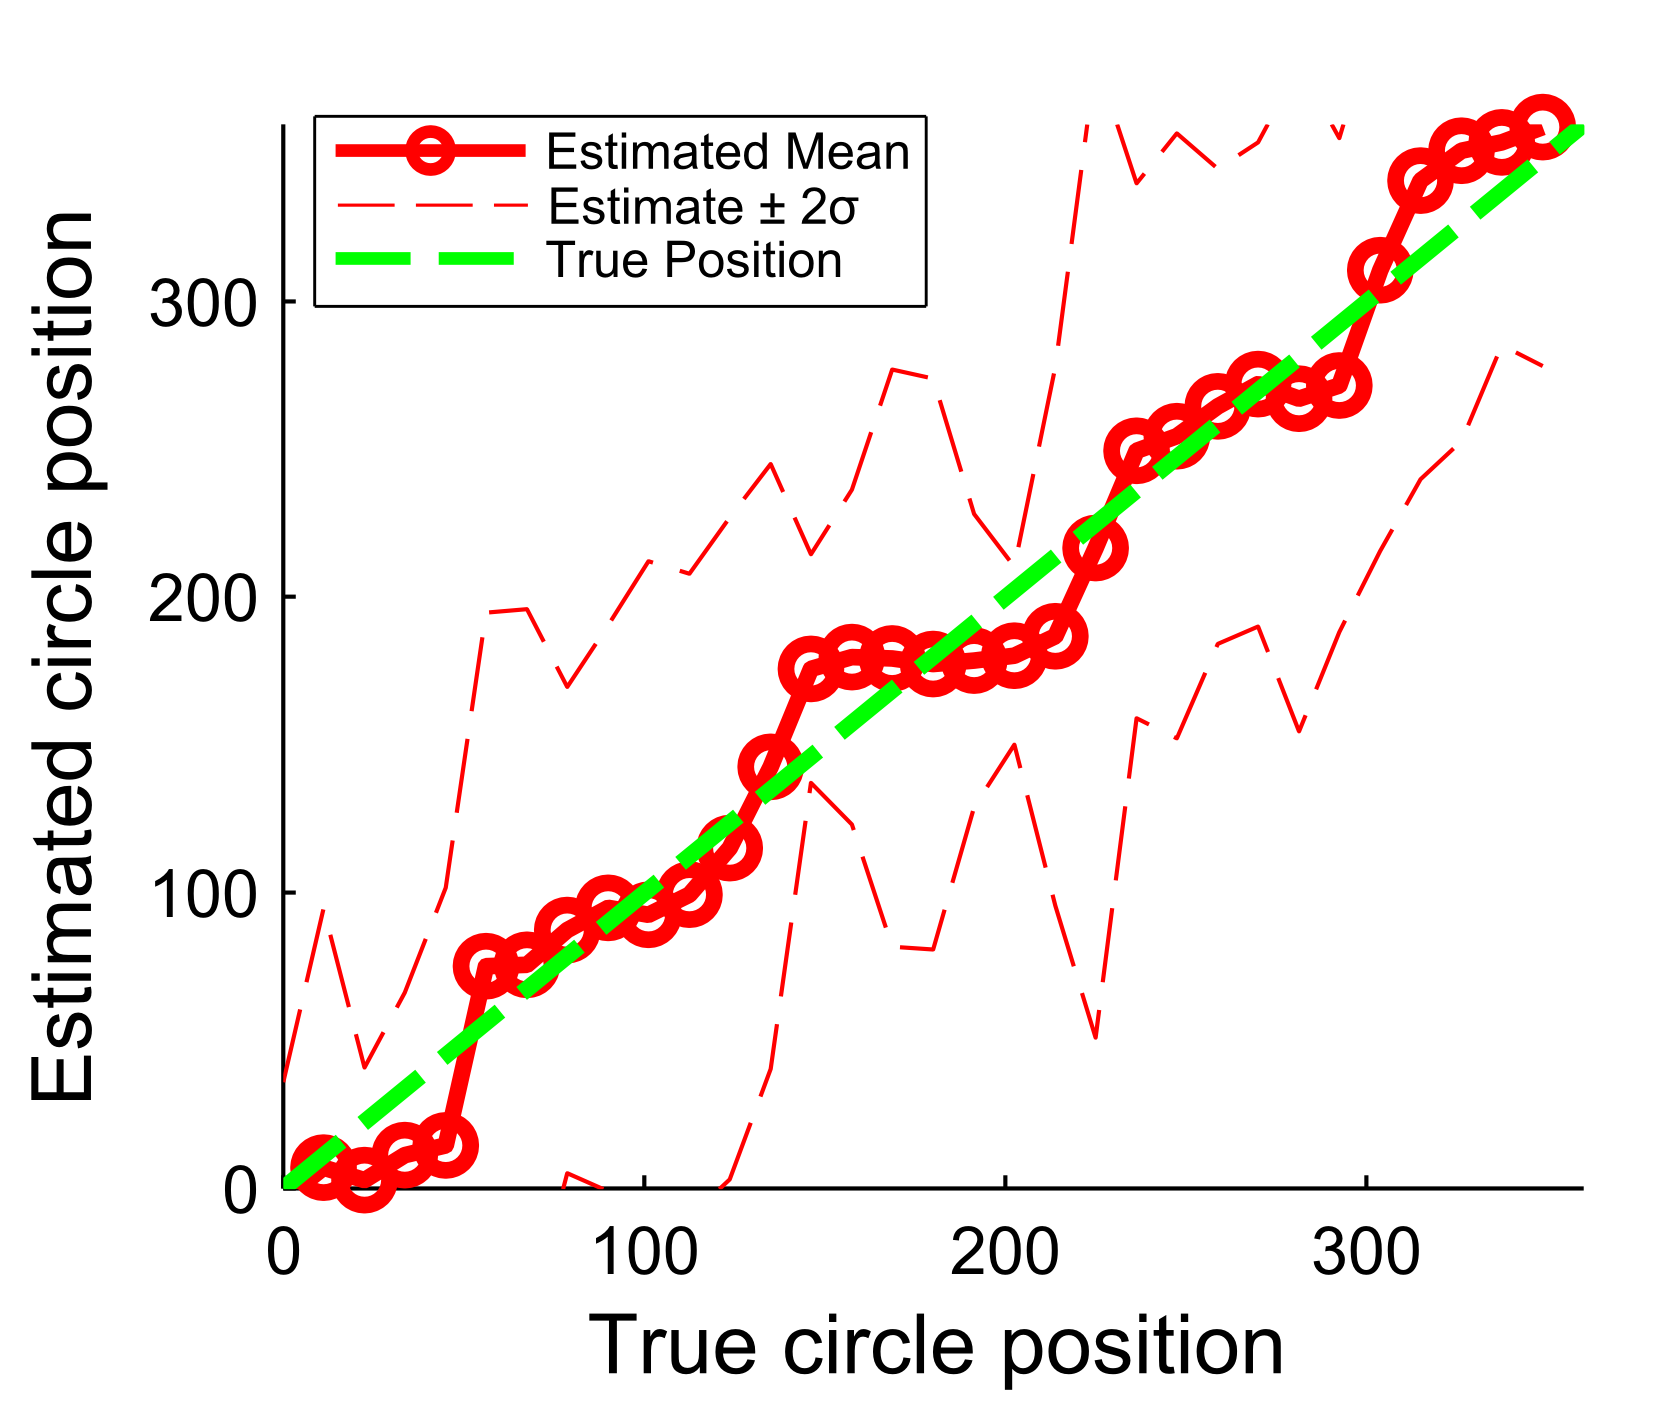
\includegraphics[scale=1]{line_circular_fusion_mean_5.png}
	\caption{}
	\label{Figure: circular_fusion_mean_5}	
	\end{subfigure}\\
	\begin{subfigure}{7cm}
	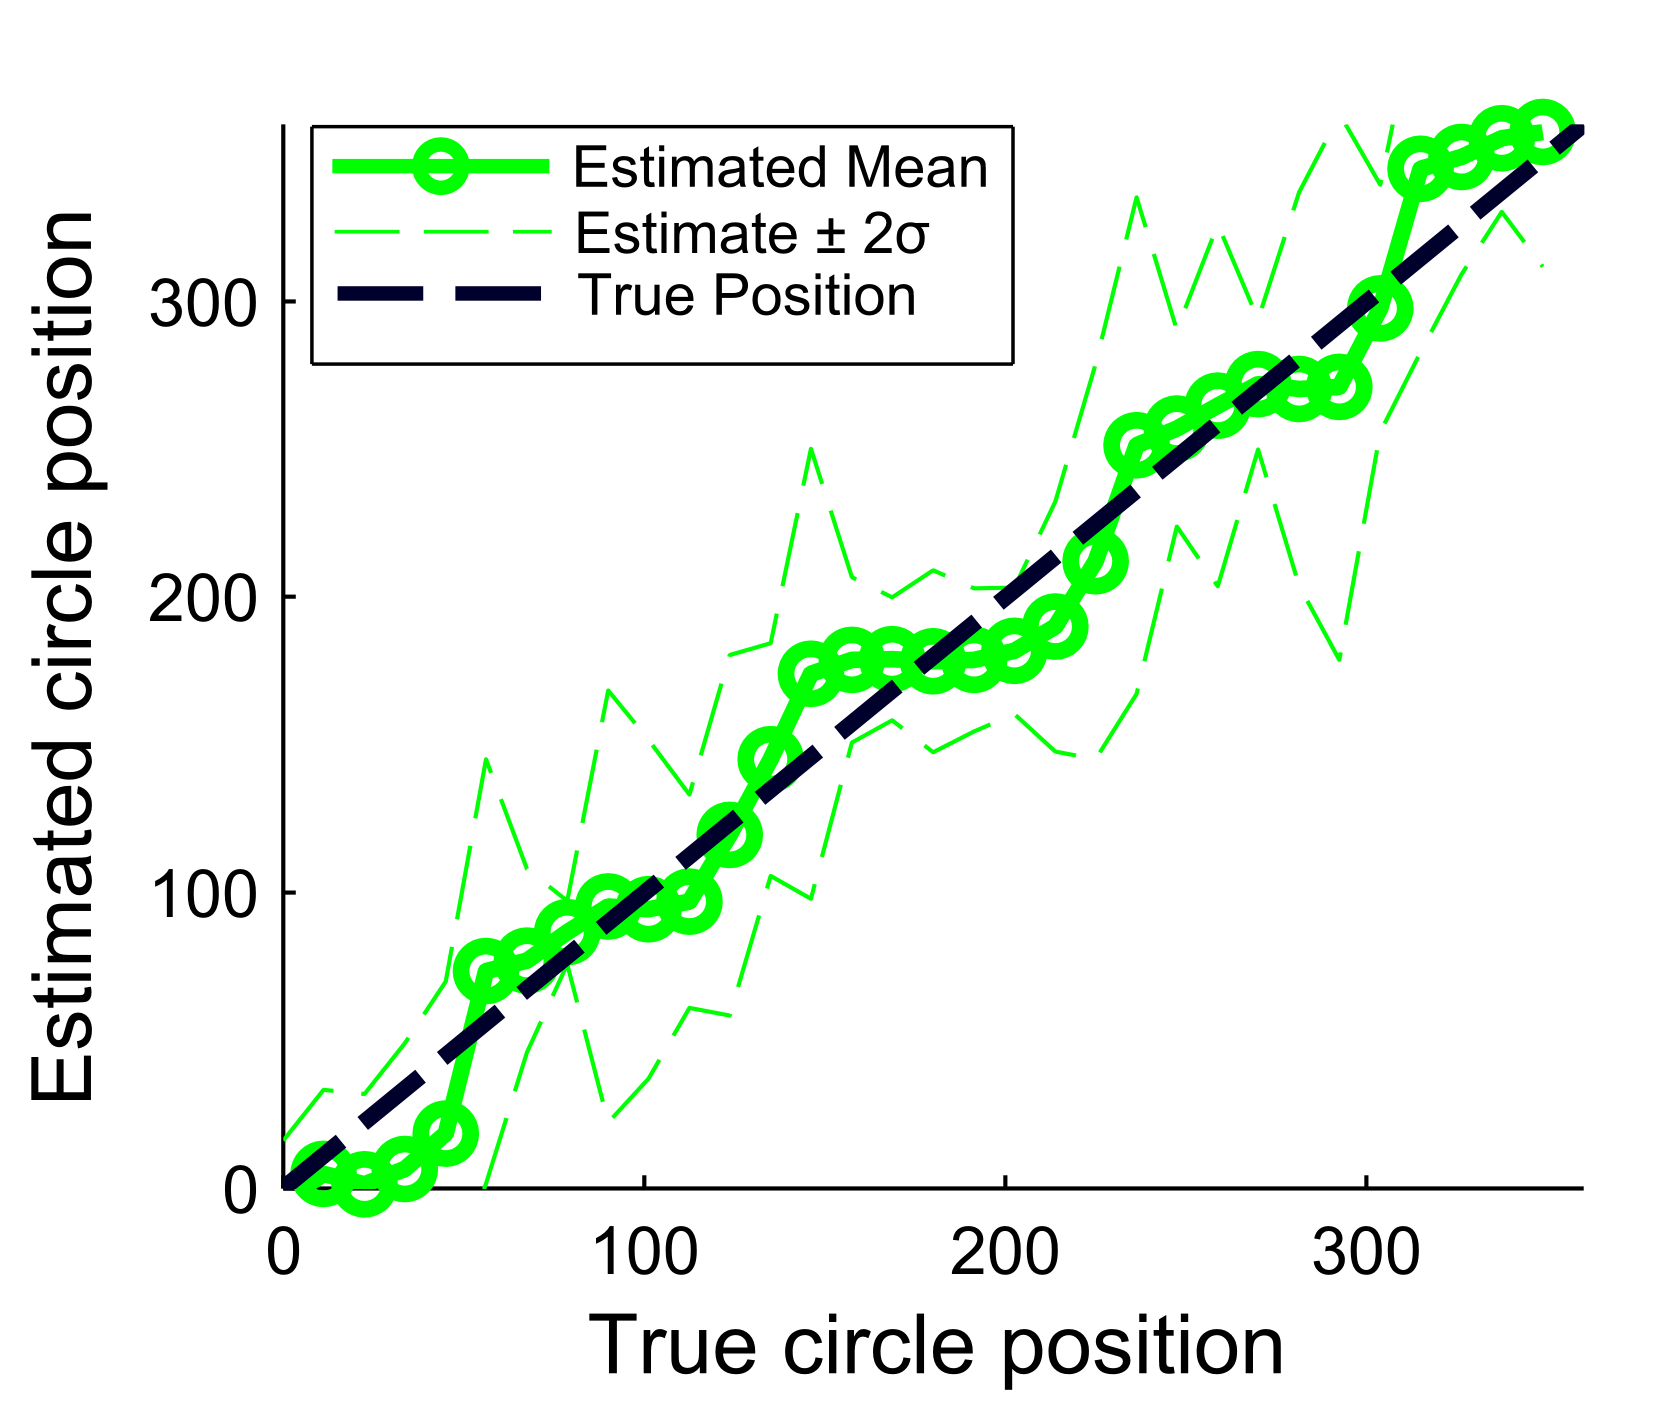
\includegraphics[scale=1]{line_circular_fusion_mean_10.png}
	\caption{}	
	\label{Figure: circular_fusion_mean_10}
	\end{subfigure}
	\begin{subfigure}{7cm}
	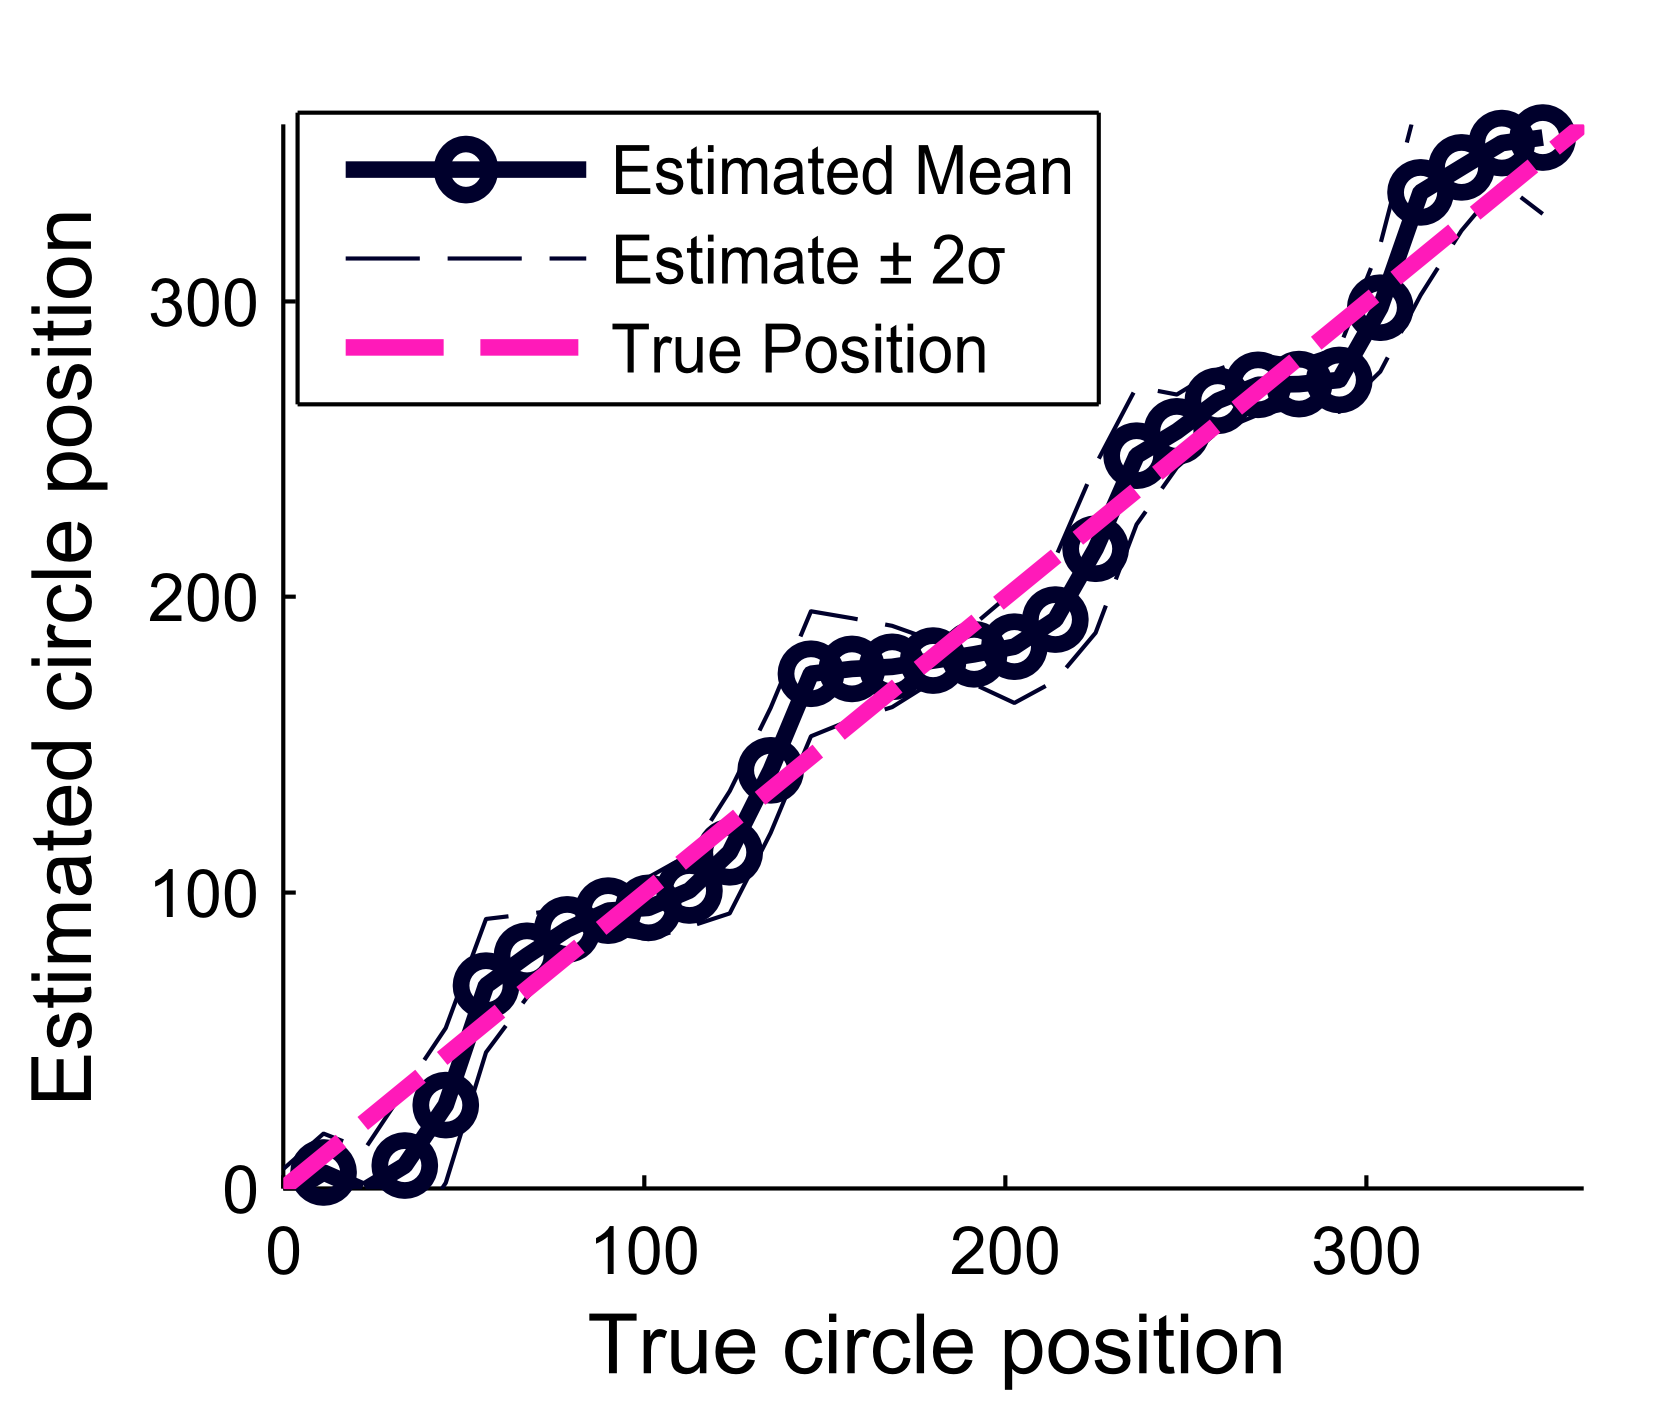
\includegraphics[scale=1]{line_circular_fusion_mean_40.png}
	\caption{}	
	\label{Figure: circular_fusion_mean_40}
	\end{subfigure}
	\label{Figure: circular_fusion_mean}
	\caption{The mean performance of estimating the circle's position from the circular response. The mean line is the expectation value of the posterior distribution taken from 50 simulations. The standard deviation is for the spread of expectation values over the simulations - not the spread in individual posteriors. The data was collected for varying numbers of responses with \subref{Figure: circular_fusion_mean_1}) 1 response \subref{Figure: circular_fusion_mean_5}) 5 responses \subref{Figure: circular_fusion_mean_10}) 10 responses \subref{Figure: circular_fusion_mean_40})40 responses}
\end{figure}


\begin{figure}
	\centering
	\begin{subfigure}{7cm}
	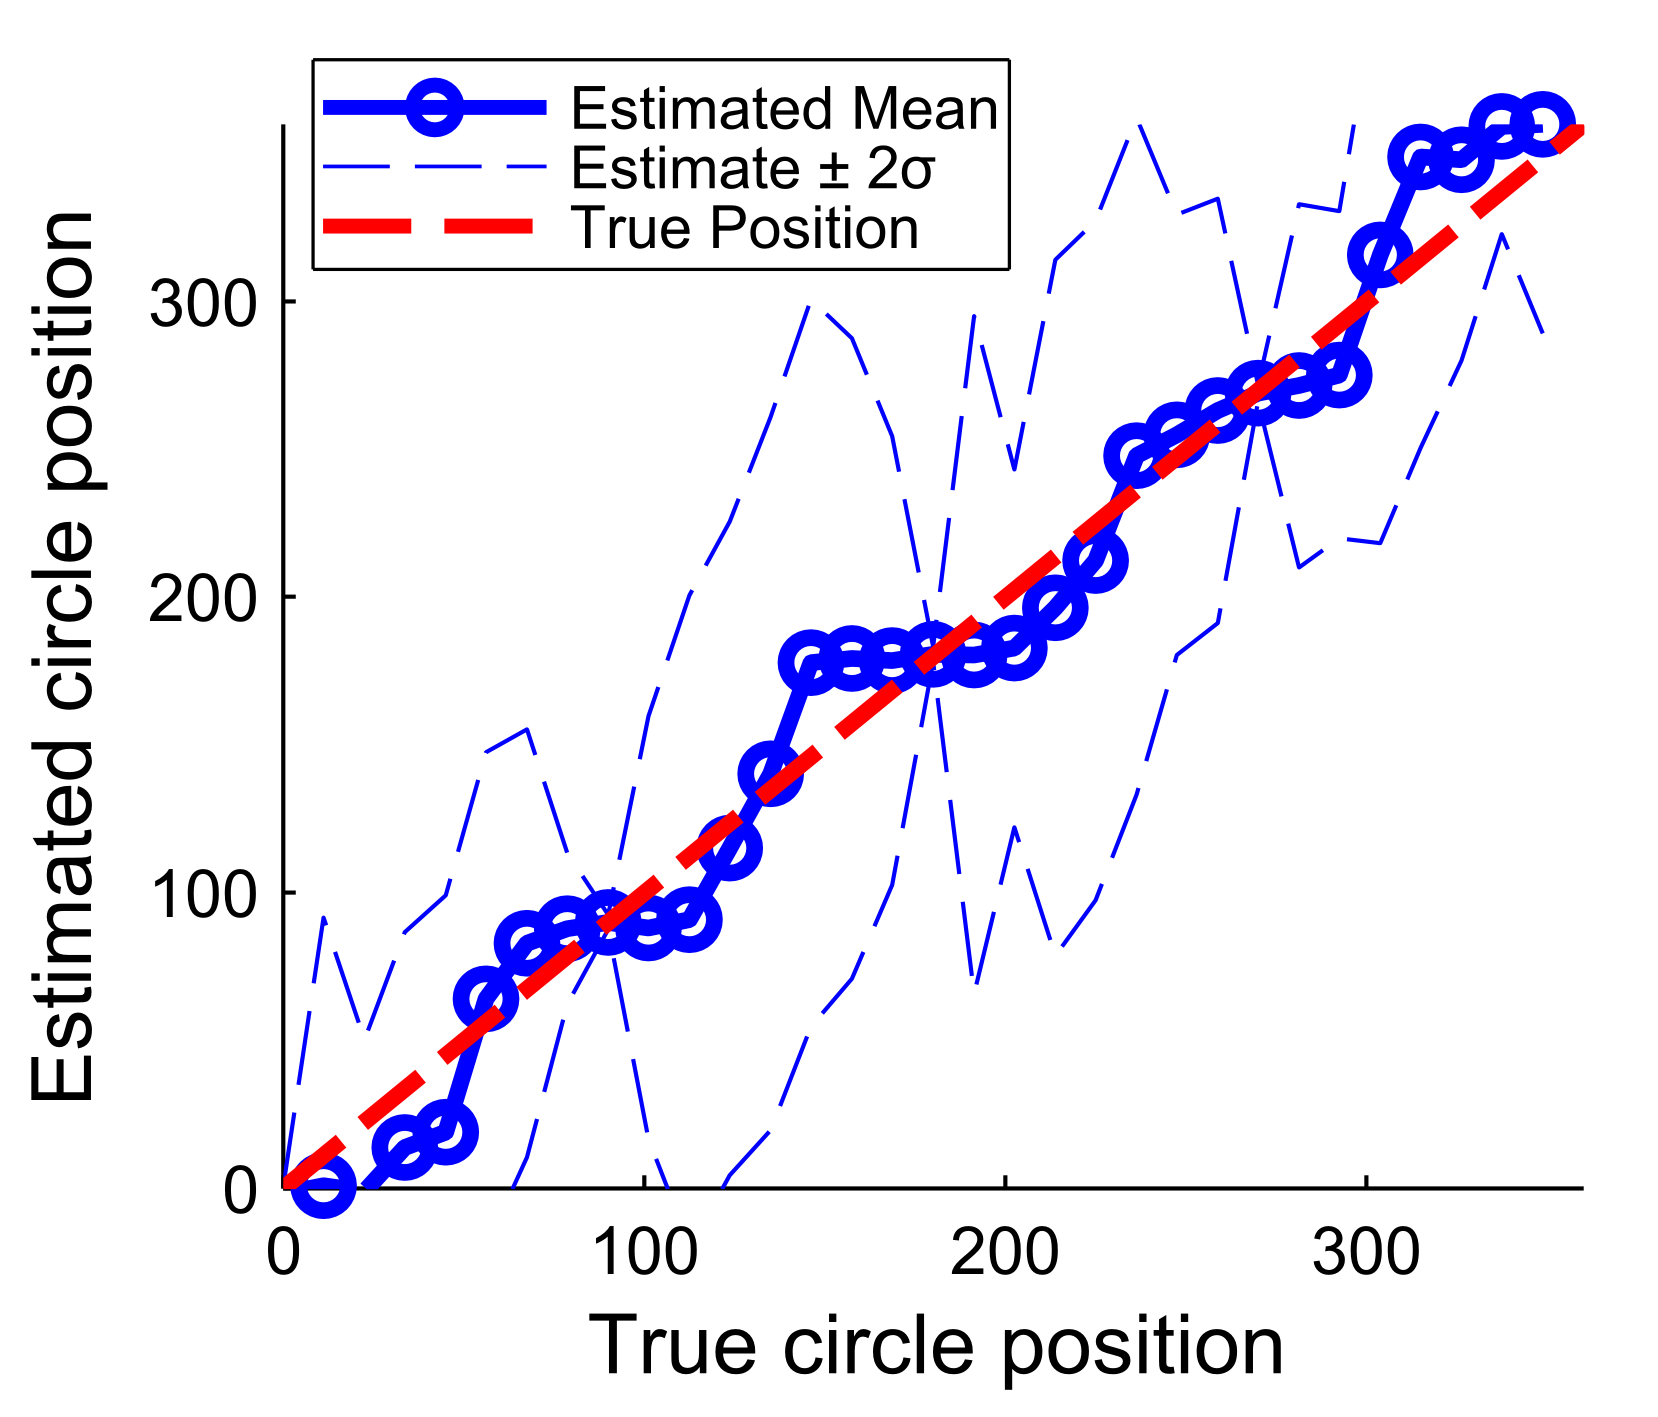
\includegraphics[scale=1]{circular_line_fusion_mean_1report_gold.png}
	\caption{}	
	\label{Figure: circular_fusion_mean_1_gold}
	\end{subfigure}
	\begin{subfigure}{7cm}
	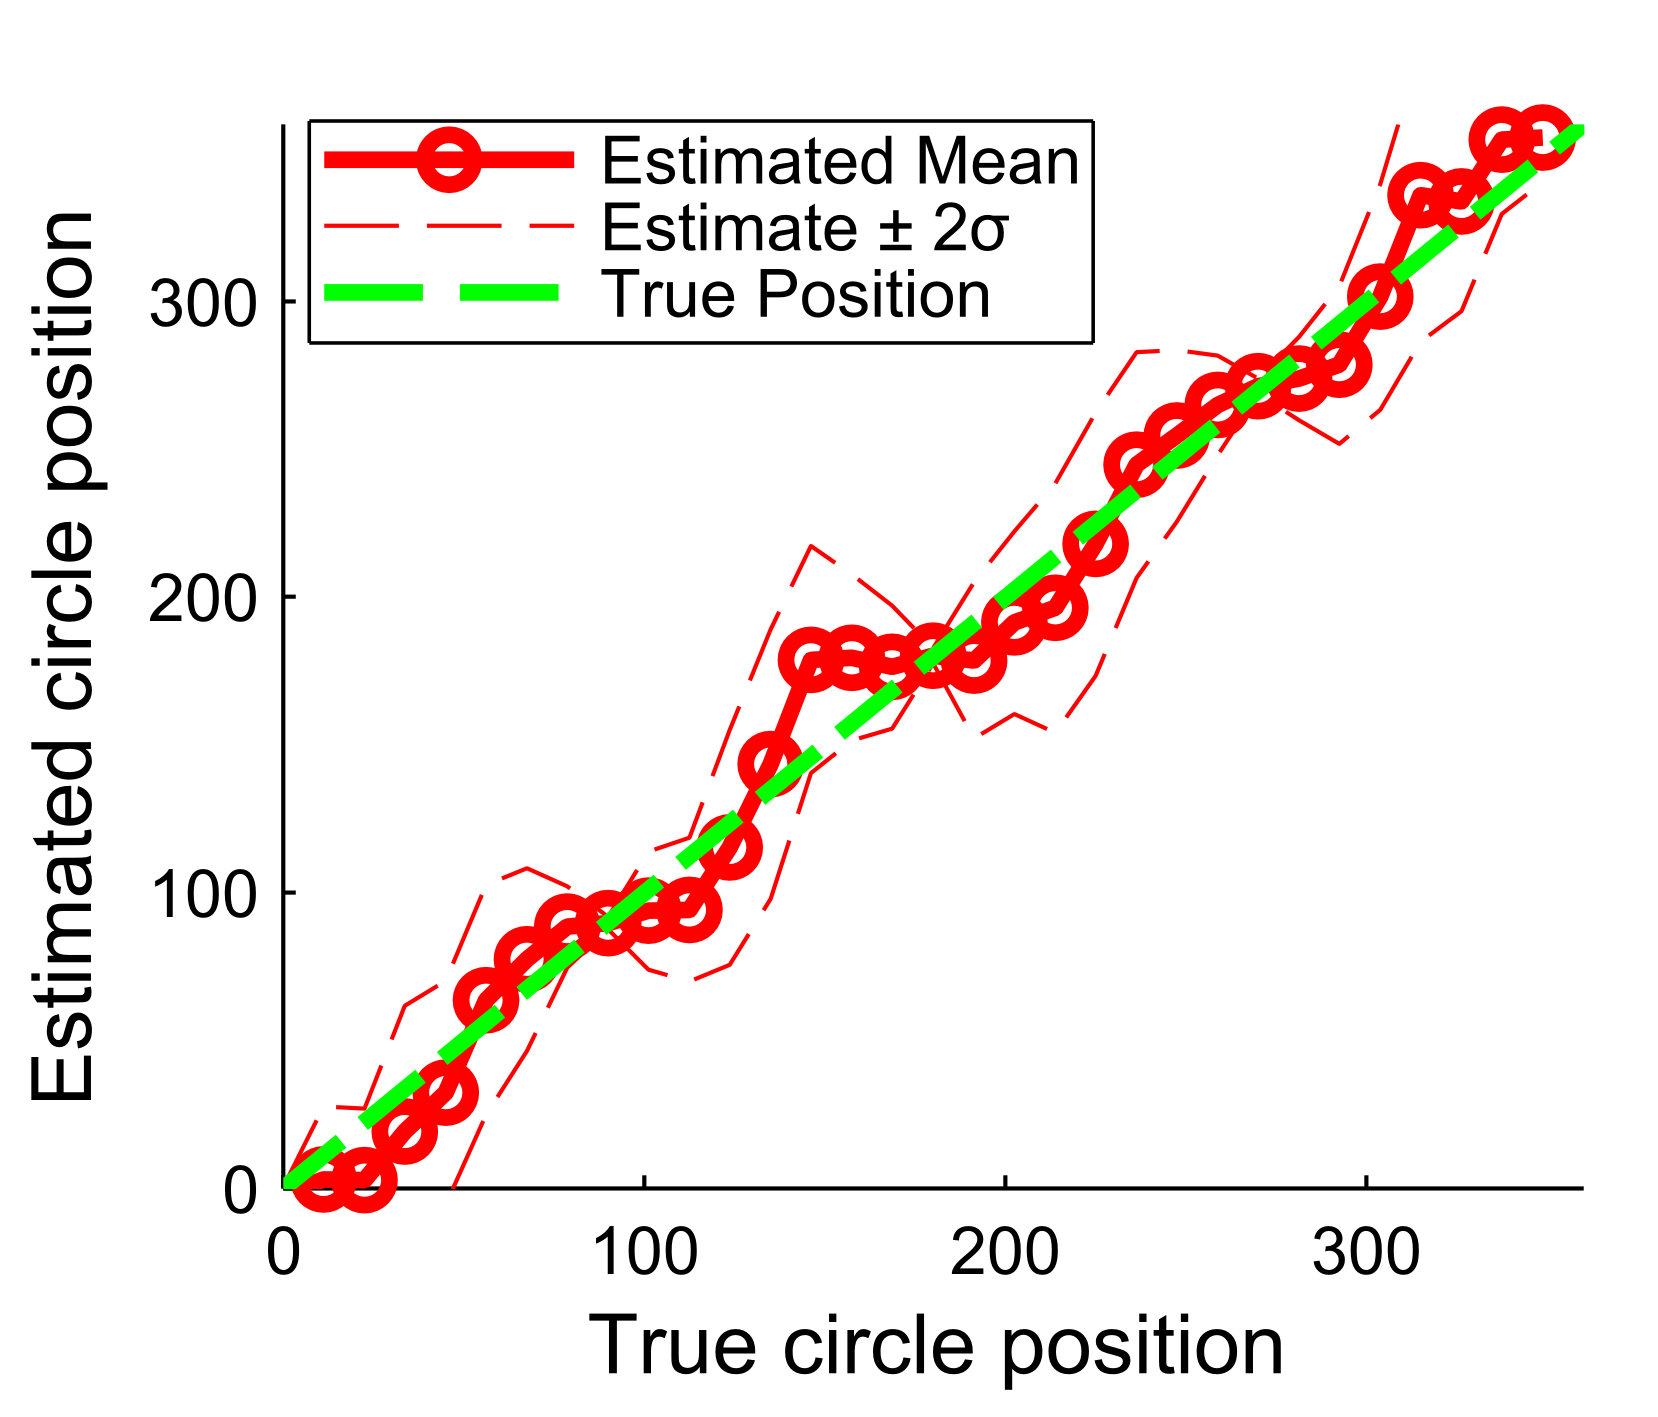
\includegraphics[scale=1]{line_circular_fusion_mean_5_gold.png}
	\caption{}
	\label{Figure: circular_fusion_mean_5_gold}	
	\end{subfigure}\\
	\begin{subfigure}{7cm}
	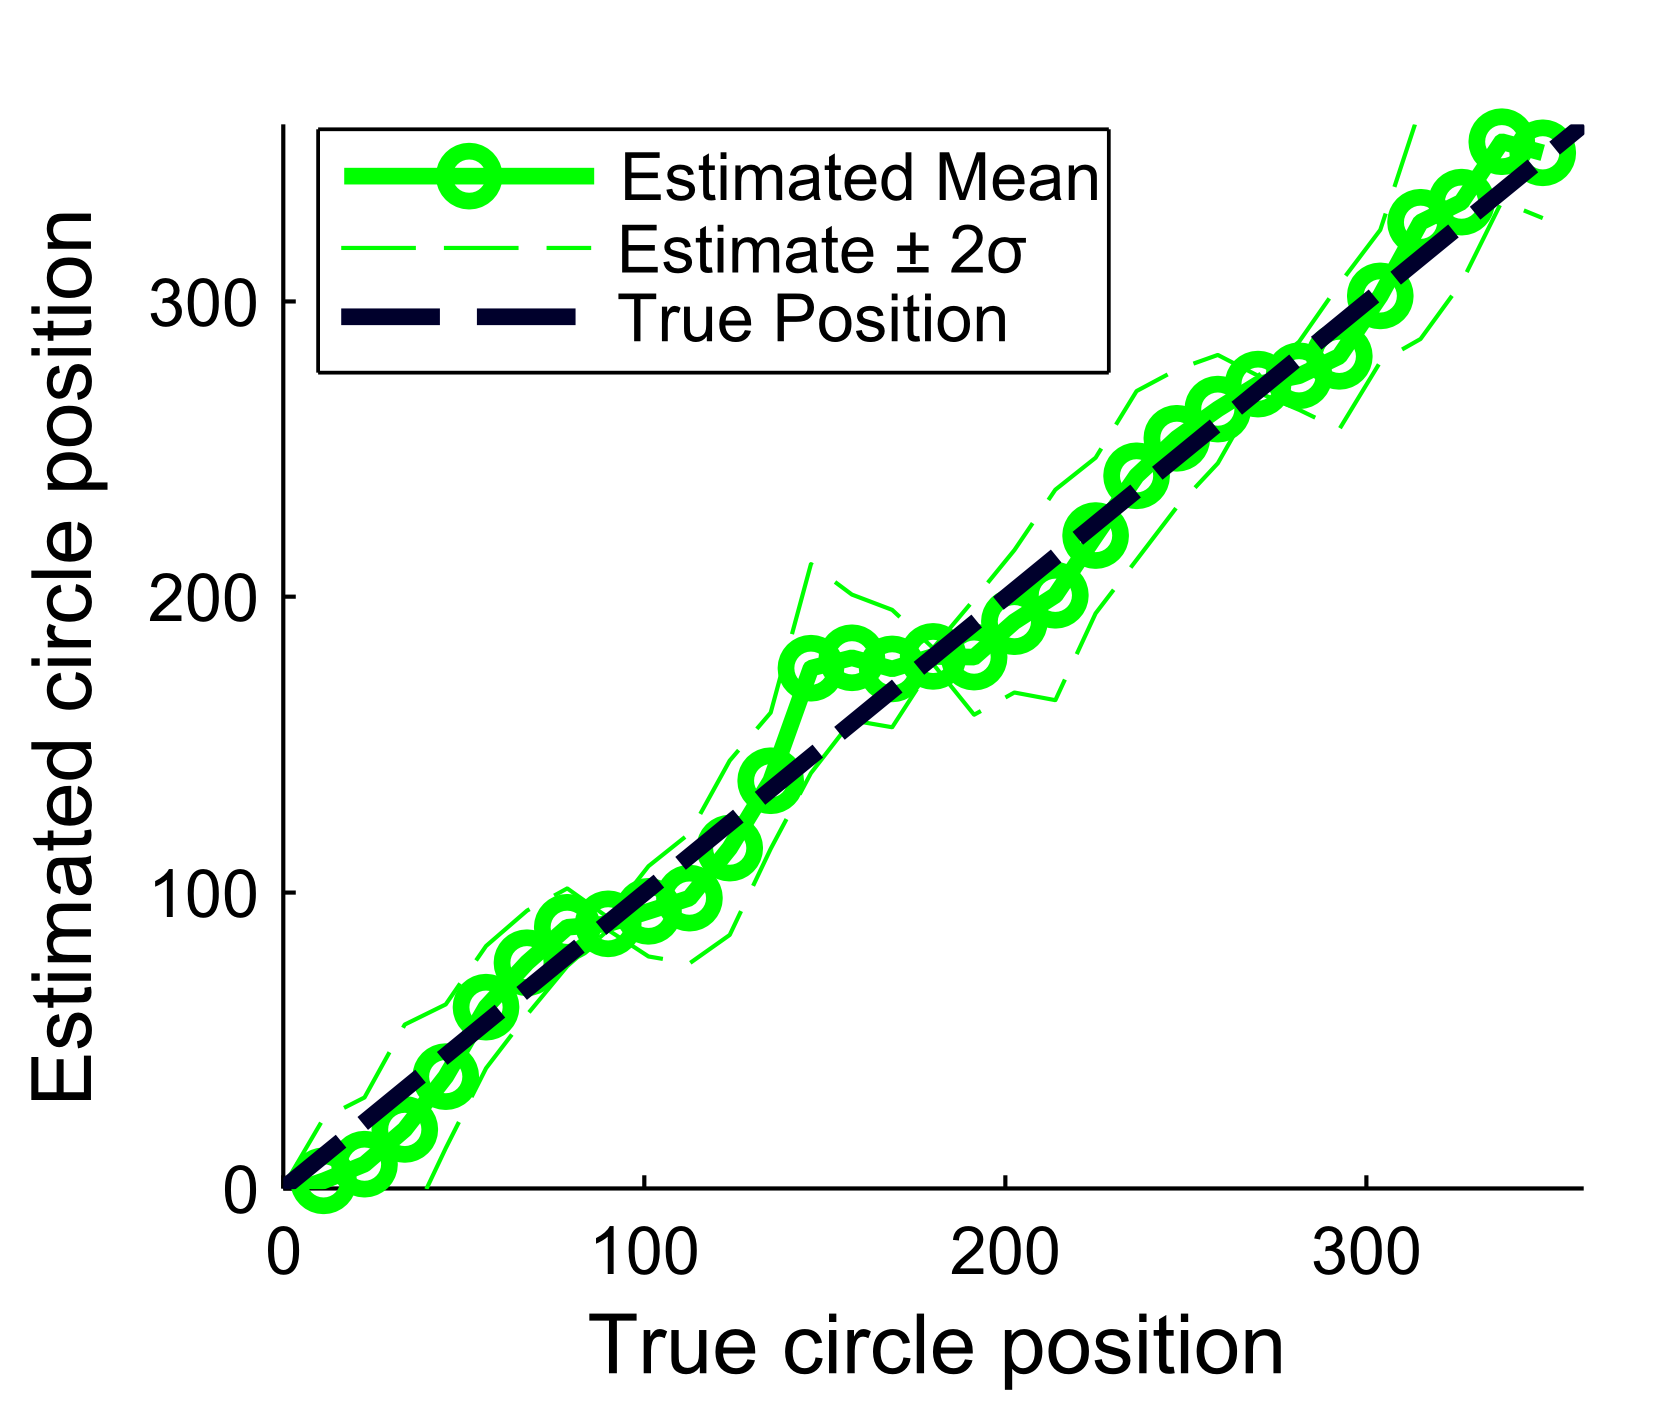
\includegraphics[scale=1]{line_circular_fusion_mean_10_gold.png}
	\caption{}	
	\label{Figure: circular_fusion_mean_10_gold}
	\end{subfigure}
	\begin{subfigure}{7cm}
	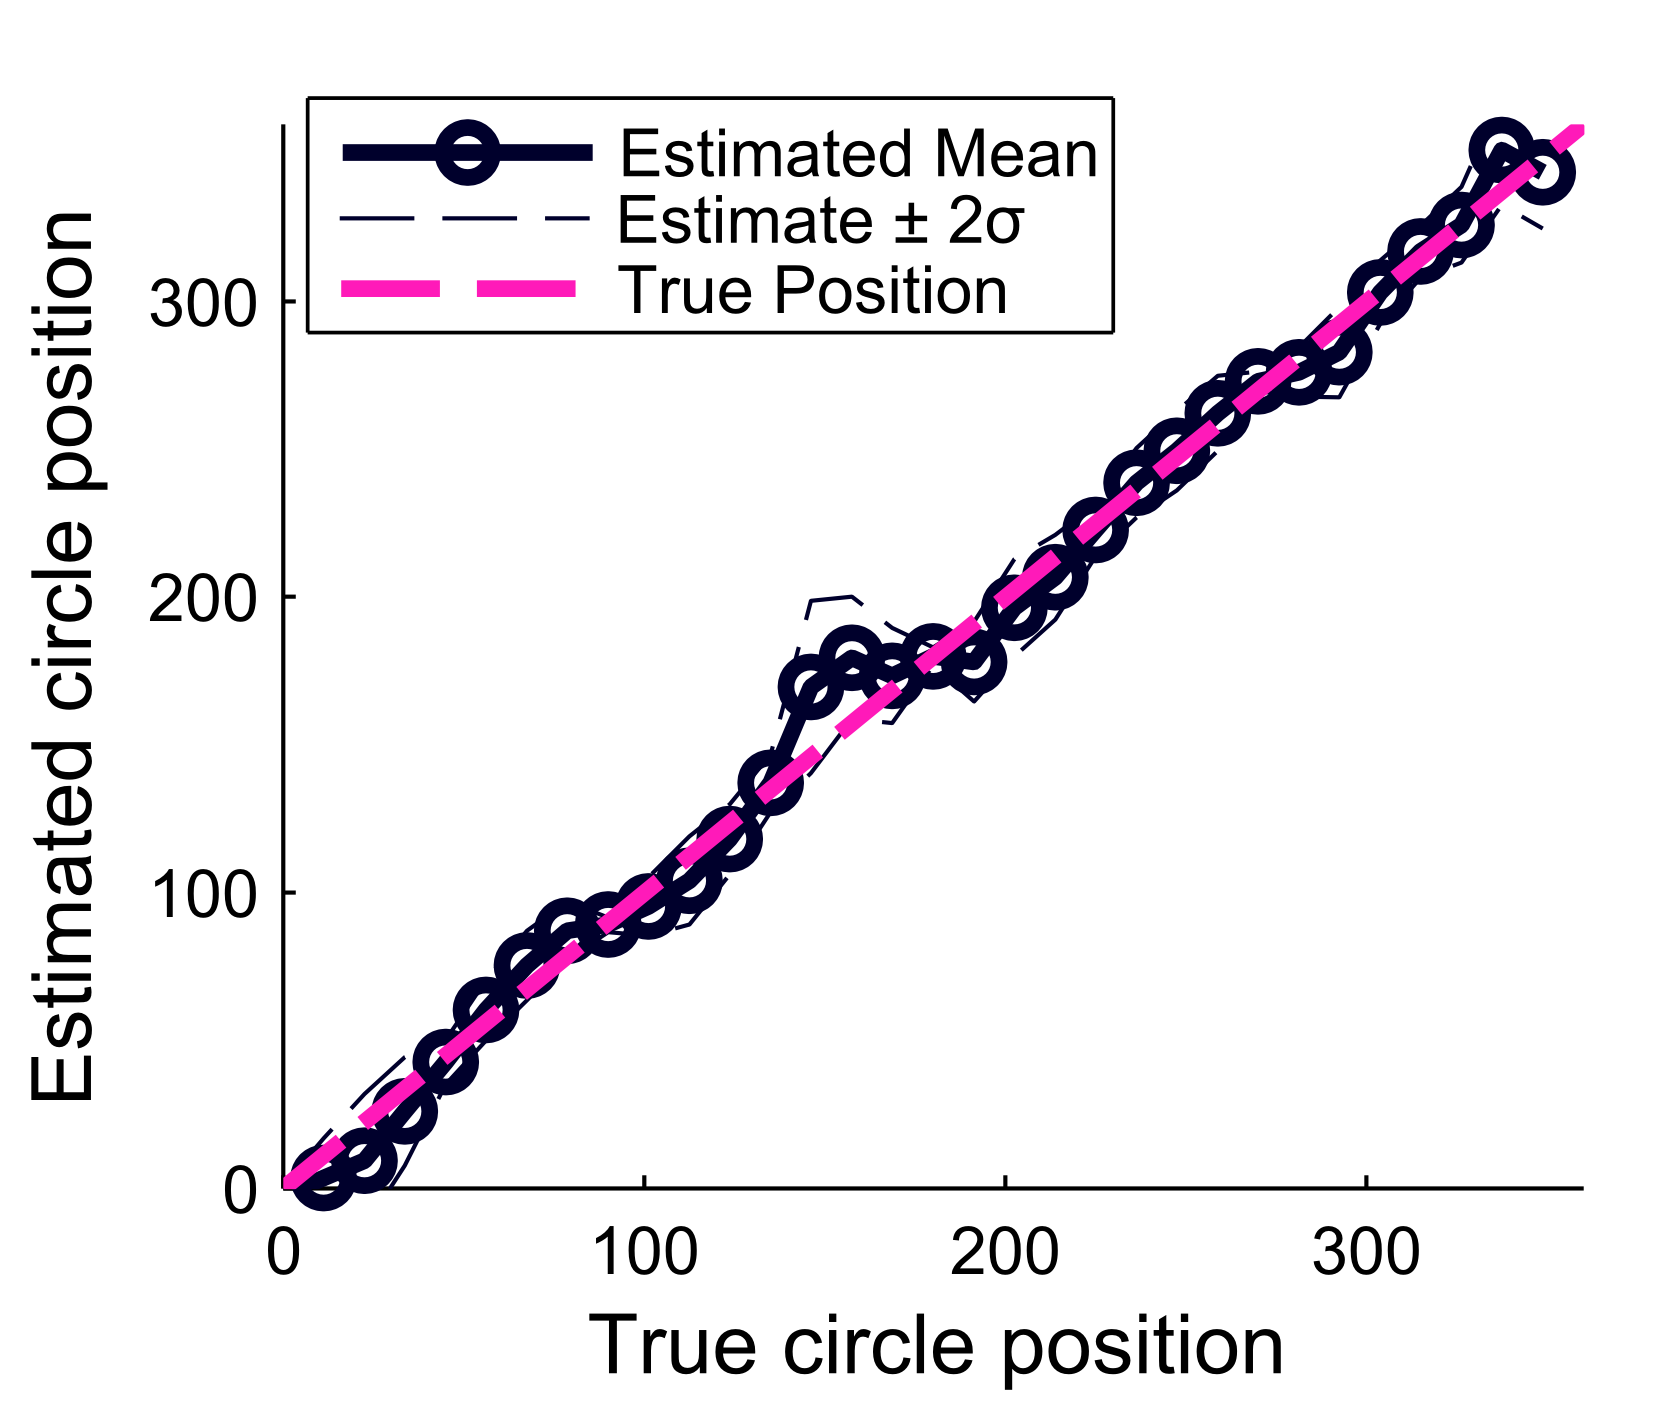
\includegraphics[scale=1]{line_circular_fusion_mean_40_gold.png}
	\caption{}	
	\label{Figure: circular_fusion_mean_40_gold}
	\end{subfigure}
	\label{Figure: circular_fusion_mean_gold}
	\caption{The mean performance of estimating the circle's position from the circular response gold data. The mean line is the expectation value of the posterior distribution taken from 50 simulations. The standard deviation is for the spread of expectation values over the simulations - not the spread in individual posteriors. The data was collected for varying numbers of responses with \subref{Figure: circular_fusion_mean_1_gold}) 1 response \subref{Figure: circular_fusion_mean_5_gold}) 5 responses \subref{Figure: circular_fusion_mean_10_gold}) 10 responses \subref{Figure: circular_fusion_mean_40_gold})40 responses}
\end{figure}
%\include{Conclusions}
\chapter{Data Fusion} \label{Chapter: Derivations}

\section{Hard Soft Data fusion}

\newcommand{\CP}[2]{\ensuremath{p(#1|#2)}} %%Conditional Prob

\newcommand{\tstamp}{\ensuremath{k}}
\newcommand{\state}{\ensuremath{X}}
\newcommand{\stateTime}{\ensuremath{\state_{\tstamp}}}
\newcommand{\stateTimePri}{\ensuremath{\state_{\tstamp-1}}}

\newcommand{\hard}{\ensuremath{H}}
\newcommand{\hardTime}{\ensuremath{\hard_\tstamp}}
\newcommand{\hardRange}[2]{\ensuremath{\hard_{#1:#2}}}
\newcommand{\hardUpToPri}{\ensuremath{\hardRange{1}{\tstamp-1}}}
\newcommand{\hardUpToTime}{\ensuremath{\hardRange{1}{\tstamp}}}

\newcommand{\soft}{\ensuremath{S}}
\newcommand{\softTime}{\ensuremath{\soft_\tstamp}}
\newcommand{\softRange}[2]{\ensuremath{\soft_{#1:#2}}}
\newcommand{\softUpToPri}{\ensuremath{\softRange{1}{\tstamp-1}}}
\newcommand{\softUpToTime}{\ensuremath{\softRange{1}{\tstamp}}}

Chapman-Kolmogrov:
\begin{equation}
\CP{\stateTime}{\hardUpToPri,\softUpToPri}= \int \CP{\stateTime}{\stateTimePri}\CP{\stateTimePri}{\hardUpToPri,\softUpToPri} d\stateTimePri
\end{equation}

Hard Update:
\begin{equation}
\CP{\stateTime}{\hardUpToTime,\softUpToPri}=\frac{\CP{\hardUpToTime}{\stateTime}\CP{\stateTime}{\softUpToPri}}{\int \CP{\hardUpToTime}{\stateTime}\CP{\stateTime}{\hardUpToPri,\softUpToPri}d\stateTime}
\end{equation}

Soft Update:
\begin{equation}
\CP{\stateTime}{\hardUpToTime,\softUpToTime}= \frac{\CP{\softUpToTime}{\stateTime}\CP{\stateTime}{\hardUpToTime, \softUpToPri}}{\int \CP{\hardUpToTime}{\stateTime}\CP{\hardUpToTime}{\softUpToTime}d\stateTime}
\end{equation}


\appendix
\include{AppendixA}
\backmatter
\bibliographystyle{ecs}
\bibliography{ECS}
\end{document}
%% ----------------------------------------------------------------